\documentclass{book}
\usepackage[a4paper,top=2.5cm,bottom=2.5cm,left=2.5cm,right=2.5cm]{geometry}
\usepackage{makeidx}
\usepackage{natbib}
\usepackage{graphicx}
\usepackage{multicol}
\usepackage{float}
\usepackage{listings}
\usepackage{color}
\usepackage{ifthen}
\usepackage[table]{xcolor}
\usepackage{textcomp}
\usepackage{alltt}
\usepackage{ifpdf}
\ifpdf
\usepackage[pdftex,
            pagebackref=true,
            colorlinks=true,
            linkcolor=blue,
            unicode
           ]{hyperref}
\else
\usepackage[ps2pdf,
            pagebackref=true,
            colorlinks=true,
            linkcolor=blue,
            unicode
           ]{hyperref}
\usepackage{pspicture}
\fi
\usepackage[utf8]{inputenc}
\usepackage{mathptmx}
\usepackage[scaled=.90]{helvet}
\usepackage{courier}
\usepackage{sectsty}
\usepackage[titles]{tocloft}
\usepackage{doxygen}
\lstset{language=C++,inputencoding=utf8,basicstyle=\footnotesize,breaklines=true,breakatwhitespace=true,tabsize=8,numbers=left }
\makeindex
\setcounter{tocdepth}{3}
\renewcommand{\footrulewidth}{0.4pt}
\renewcommand{\familydefault}{\sfdefault}
\hfuzz=15pt
\setlength{\emergencystretch}{15pt}
\hbadness=750
\tolerance=750
\begin{document}
\hypersetup{pageanchor=false,citecolor=blue}
\begin{titlepage}
\vspace*{7cm}
\begin{center}
{\Large Sharpenguin \\[1ex]\large The C\# Club Penguin Client }\\
\vspace*{1cm}
{\large Generated by Doxygen 1.8.1}\\
\vspace*{0.5cm}
{\small Sun Nov 4 2012 21:49:53}\\
\end{center}
\end{titlepage}
\clearemptydoublepage
\pagenumbering{roman}
\tableofcontents
\clearemptydoublepage
\pagenumbering{arabic}
\hypersetup{pageanchor=true,citecolor=blue}
\chapter{Namespace Index}
\section{Namespace List}
Here is a list of all documented namespaces with brief descriptions\-:\begin{DoxyCompactList}
\item\contentsline{section}{\hyperlink{namespaceProcurios}{Procurios} }{\pageref{namespaceProcurios}}{}
\item\contentsline{section}{\hyperlink{namespaceProcurios_1_1Public}{Procurios.\-Public} }{\pageref{namespaceProcurios_1_1Public}}{}
\item\contentsline{section}{\hyperlink{namespaceSharpenguin}{Sharpenguin} }{\pageref{namespaceSharpenguin}}{}
\item\contentsline{section}{\hyperlink{namespaceSharpenguin_1_1Data}{Sharpenguin.\-Data} }{\pageref{namespaceSharpenguin_1_1Data}}{}
\item\contentsline{section}{\hyperlink{namespaceSharpenguin_1_1Exceptions}{Sharpenguin.\-Exceptions} }{\pageref{namespaceSharpenguin_1_1Exceptions}}{}
\item\contentsline{section}{\hyperlink{namespaceSharpenguin_1_1Net}{Sharpenguin.\-Net} }{\pageref{namespaceSharpenguin_1_1Net}}{}
\item\contentsline{section}{\hyperlink{namespaceSharpenguin_1_1Out}{Sharpenguin.\-Out} }{\pageref{namespaceSharpenguin_1_1Out}}{}
\item\contentsline{section}{\hyperlink{namespaceSharpenguin_1_1Phrase}{Sharpenguin.\-Phrase} }{\pageref{namespaceSharpenguin_1_1Phrase}}{}
\item\contentsline{section}{\hyperlink{namespaceSharpenguin_1_1Security}{Sharpenguin.\-Security} }{\pageref{namespaceSharpenguin_1_1Security}}{}
\item\contentsline{section}{\hyperlink{namespaceSharpenguin_1_1Xt}{Sharpenguin.\-Xt} }{\pageref{namespaceSharpenguin_1_1Xt}}{}
\end{DoxyCompactList}

\chapter{Class Index}
\section{Class Hierarchy}
This inheritance list is sorted roughly, but not completely, alphabetically\-:\begin{DoxyCompactList}
\item \contentsline{section}{Sharpenguin.\-Net.\-Penguin\-Socket.\-Buffer\-State}{\pageref{classSharpenguin_1_1Net_1_1PenguinSocket_1_1BufferState}}{}
\item \contentsline{section}{Sharpenguin.\-Data.\-C\-P\-Crumbs}{\pageref{classSharpenguin_1_1Data_1_1CPCrumbs}}{}
\item \contentsline{section}{Sharpenguin.\-Data.\-Crumb\-Collection}{\pageref{classSharpenguin_1_1Data_1_1CrumbCollection}}{}
\item \contentsline{section}{Sharpenguin.\-Xt.\-Handler\-Table}{\pageref{classSharpenguin_1_1Xt_1_1HandlerTable}}{}
\item \contentsline{section}{Procurios.\-Public.\-J\-S\-O\-N}{\pageref{classProcurios_1_1Public_1_1JSON}}{}
\item \contentsline{section}{Sharpenguin.\-Penguin\-Base}{\pageref{classSharpenguin_1_1PenguinBase}}{}
\begin{DoxyCompactList}
\item \contentsline{section}{Sharpenguin.\-Tasks}{\pageref{classSharpenguin_1_1Tasks}}{}
\begin{DoxyCompactList}
\item \contentsline{section}{Sharpenguin.\-Penguin}{\pageref{classSharpenguin_1_1Penguin}}{}
\end{DoxyCompactList}
\end{DoxyCompactList}
\item \contentsline{section}{Sharpenguin.\-Exceptions.\-Penguin\-Exception}{\pageref{classSharpenguin_1_1Exceptions_1_1PenguinException}}{}
\begin{DoxyCompactList}
\item \contentsline{section}{Sharpenguin.\-Exceptions.\-Early\-Join\-Exception}{\pageref{classSharpenguin_1_1Exceptions_1_1EarlyJoinException}}{}
\item \contentsline{section}{Sharpenguin.\-Exceptions.\-Invalid\-A\-P\-I\-Exception}{\pageref{classSharpenguin_1_1Exceptions_1_1InvalidAPIException}}{}
\item \contentsline{section}{Sharpenguin.\-Exceptions.\-Invalid\-Config\-Exception}{\pageref{classSharpenguin_1_1Exceptions_1_1InvalidConfigException}}{}
\item \contentsline{section}{Sharpenguin.\-Exceptions.\-Invalid\-Xt\-Exception}{\pageref{classSharpenguin_1_1Exceptions_1_1InvalidXtException}}{}
\item \contentsline{section}{Sharpenguin.\-Exceptions.\-Non\-Existant\-Crumb\-Exception}{\pageref{classSharpenguin_1_1Exceptions_1_1NonExistantCrumbException}}{}
\item \contentsline{section}{Sharpenguin.\-Exceptions.\-Non\-Existant\-Player\-Exception}{\pageref{classSharpenguin_1_1Exceptions_1_1NonExistantPlayerException}}{}
\item \contentsline{section}{Sharpenguin.\-Exceptions.\-Phrase\-Chat\-Error\-Exception}{\pageref{classSharpenguin_1_1Exceptions_1_1PhraseChatErrorException}}{}
\end{DoxyCompactList}
\item \contentsline{section}{Sharpenguin.\-Data.\-Penguin\-Packet}{\pageref{classSharpenguin_1_1Data_1_1PenguinPacket}}{}
\item \contentsline{section}{Sharpenguin.\-Data.\-Penguin\-Room}{\pageref{classSharpenguin_1_1Data_1_1PenguinRoom}}{}
\item \contentsline{section}{Sharpenguin.\-Net.\-Penguin\-Socket}{\pageref{classSharpenguin_1_1Net_1_1PenguinSocket}}{}
\item \contentsline{section}{Sharpenguin.\-Data.\-Player}{\pageref{classSharpenguin_1_1Data_1_1Player}}{}
\begin{DoxyCompactList}
\item \contentsline{section}{Sharpenguin.\-Data.\-My\-Player}{\pageref{classSharpenguin_1_1Data_1_1MyPlayer}}{}
\end{DoxyCompactList}
\item \contentsline{section}{Sharpenguin.\-Data.\-Player\-Item}{\pageref{classSharpenguin_1_1Data_1_1PlayerItem}}{}
\item \contentsline{section}{Sharpenguin.\-Data.\-Player\-Position}{\pageref{classSharpenguin_1_1Data_1_1PlayerPosition}}{}
\item \contentsline{section}{Sharpenguin.\-Xt.\-Xt\-Parser}{\pageref{classSharpenguin_1_1Xt_1_1XtParser}}{}
\end{DoxyCompactList}

\chapter{Class Index}
\section{Class List}
Here are the classes, structs, unions and interfaces with brief descriptions\-:\begin{DoxyCompactList}
\item\contentsline{section}{\hyperlink{classSharpenguin_1_1Net_1_1BufferState}{Sharpenguin.\-Net.\-Buffer\-State} }{\pageref{classSharpenguin_1_1Net_1_1BufferState}}{}
\item\contentsline{section}{\hyperlink{classSharpenguin_1_1Net_1_1ConnectState}{Sharpenguin.\-Net.\-Connect\-State} }{\pageref{classSharpenguin_1_1Net_1_1ConnectState}}{}
\item\contentsline{section}{\hyperlink{classSharpenguin_1_1Data_1_1CPCrumbs}{Sharpenguin.\-Data.\-C\-P\-Crumbs} }{\pageref{classSharpenguin_1_1Data_1_1CPCrumbs}}{}
\item\contentsline{section}{\hyperlink{classSharpenguin_1_1Data_1_1CrumbCollection}{Sharpenguin.\-Data.\-Crumb\-Collection} }{\pageref{classSharpenguin_1_1Data_1_1CrumbCollection}}{}
\item\contentsline{section}{\hyperlink{classSharpenguin_1_1Exceptions_1_1EarlyJoinException}{Sharpenguin.\-Exceptions.\-Early\-Join\-Exception} }{\pageref{classSharpenguin_1_1Exceptions_1_1EarlyJoinException}}{}
\item\contentsline{section}{\hyperlink{classSharpenguin_1_1Xt_1_1HandlerTable}{Sharpenguin.\-Xt.\-Handler\-Table} }{\pageref{classSharpenguin_1_1Xt_1_1HandlerTable}}{}
\item\contentsline{section}{\hyperlink{classSharpenguin_1_1Exceptions_1_1InvalidAPIException}{Sharpenguin.\-Exceptions.\-Invalid\-A\-P\-I\-Exception} }{\pageref{classSharpenguin_1_1Exceptions_1_1InvalidAPIException}}{}
\item\contentsline{section}{\hyperlink{classSharpenguin_1_1Exceptions_1_1InvalidConfigException}{Sharpenguin.\-Exceptions.\-Invalid\-Config\-Exception} }{\pageref{classSharpenguin_1_1Exceptions_1_1InvalidConfigException}}{}
\item\contentsline{section}{\hyperlink{classSharpenguin_1_1Exceptions_1_1InvalidXtException}{Sharpenguin.\-Exceptions.\-Invalid\-Xt\-Exception} }{\pageref{classSharpenguin_1_1Exceptions_1_1InvalidXtException}}{}
\item\contentsline{section}{\hyperlink{classProcurios_1_1Public_1_1JSON}{Procurios.\-Public.\-J\-S\-O\-N} \\*This class encodes and decodes \hyperlink{classProcurios_1_1Public_1_1JSON}{J\-S\-O\-N} strings. Spec. details, see \href{http://www.json.org/}{\tt http\-://www.\-json.\-org/} }{\pageref{classProcurios_1_1Public_1_1JSON}}{}
\item\contentsline{section}{\hyperlink{classSharpenguin_1_1Data_1_1MyPlayer}{Sharpenguin.\-Data.\-My\-Player} }{\pageref{classSharpenguin_1_1Data_1_1MyPlayer}}{}
\item\contentsline{section}{\hyperlink{classSharpenguin_1_1Exceptions_1_1NonExistantCrumbException}{Sharpenguin.\-Exceptions.\-Non\-Existant\-Crumb\-Exception} }{\pageref{classSharpenguin_1_1Exceptions_1_1NonExistantCrumbException}}{}
\item\contentsline{section}{\hyperlink{classSharpenguin_1_1Exceptions_1_1NonExistantPlayerException}{Sharpenguin.\-Exceptions.\-Non\-Existant\-Player\-Exception} }{\pageref{classSharpenguin_1_1Exceptions_1_1NonExistantPlayerException}}{}
\item\contentsline{section}{\hyperlink{classSharpenguin_1_1Penguin}{Sharpenguin.\-Penguin} }{\pageref{classSharpenguin_1_1Penguin}}{}
\item\contentsline{section}{\hyperlink{classSharpenguin_1_1PenguinBase}{Sharpenguin.\-Penguin\-Base} }{\pageref{classSharpenguin_1_1PenguinBase}}{}
\item\contentsline{section}{\hyperlink{classSharpenguin_1_1Exceptions_1_1PenguinException}{Sharpenguin.\-Exceptions.\-Penguin\-Exception} }{\pageref{classSharpenguin_1_1Exceptions_1_1PenguinException}}{}
\item\contentsline{section}{\hyperlink{classSharpenguin_1_1Data_1_1PenguinPacket}{Sharpenguin.\-Data.\-Penguin\-Packet} }{\pageref{classSharpenguin_1_1Data_1_1PenguinPacket}}{}
\item\contentsline{section}{\hyperlink{classSharpenguin_1_1Data_1_1PenguinRoom}{Sharpenguin.\-Data.\-Penguin\-Room} }{\pageref{classSharpenguin_1_1Data_1_1PenguinRoom}}{}
\item\contentsline{section}{\hyperlink{classSharpenguin_1_1Net_1_1PenguinSocket}{Sharpenguin.\-Net.\-Penguin\-Socket} }{\pageref{classSharpenguin_1_1Net_1_1PenguinSocket}}{}
\item\contentsline{section}{\hyperlink{classSharpenguin_1_1Exceptions_1_1PhraseChatErrorException}{Sharpenguin.\-Exceptions.\-Phrase\-Chat\-Error\-Exception} }{\pageref{classSharpenguin_1_1Exceptions_1_1PhraseChatErrorException}}{}
\item\contentsline{section}{\hyperlink{classSharpenguin_1_1Data_1_1Player}{Sharpenguin.\-Data.\-Player} }{\pageref{classSharpenguin_1_1Data_1_1Player}}{}
\item\contentsline{section}{\hyperlink{classSharpenguin_1_1Data_1_1PlayerItem}{Sharpenguin.\-Data.\-Player\-Item} }{\pageref{classSharpenguin_1_1Data_1_1PlayerItem}}{}
\item\contentsline{section}{\hyperlink{classSharpenguin_1_1Data_1_1PlayerPosition}{Sharpenguin.\-Data.\-Player\-Position} }{\pageref{classSharpenguin_1_1Data_1_1PlayerPosition}}{}
\item\contentsline{section}{\hyperlink{classSharpenguin_1_1Tasks}{Sharpenguin.\-Tasks} }{\pageref{classSharpenguin_1_1Tasks}}{}
\item\contentsline{section}{\hyperlink{classSharpenguin_1_1Xt_1_1XtParser}{Sharpenguin.\-Xt.\-Xt\-Parser} }{\pageref{classSharpenguin_1_1Xt_1_1XtParser}}{}
\end{DoxyCompactList}

\chapter{Namespace Documentation}
\hypertarget{namespaceProcurios}{\section{Package Procurios}
\label{namespaceProcurios}\index{Procurios@{Procurios}}
}
\subsection*{Namespaces}
\begin{DoxyCompactItemize}
\item 
package \hyperlink{namespaceProcurios_1_1Public}{Public}
\end{DoxyCompactItemize}

\hypertarget{namespaceProcurios_1_1Public}{\section{\-Package \-Procurios.\-Public}
\label{namespaceProcurios_1_1Public}\index{\-Procurios.\-Public@{\-Procurios.\-Public}}
}
\subsection*{\-Classes}
\begin{DoxyCompactItemize}
\item 
class \hyperlink{classProcurios_1_1Public_1_1JSON}{\-J\-S\-O\-N}
\begin{DoxyCompactList}\small\item\em \-This class encodes and decodes \hyperlink{classProcurios_1_1Public_1_1JSON}{\-J\-S\-O\-N} strings. \-Spec. details, see \href{http://www.json.org/}{\tt http\-://www.\-json.\-org/}. \end{DoxyCompactList}\end{DoxyCompactItemize}

\hypertarget{namespaceSharpenguin}{\section{Package Sharpenguin}
\label{namespaceSharpenguin}\index{Sharpenguin@{Sharpenguin}}
}
\subsection*{Namespaces}
\begin{DoxyCompactItemize}
\item 
package \hyperlink{namespaceSharpenguin_1_1Data}{Data}
\item 
package \hyperlink{namespaceSharpenguin_1_1Exceptions}{Exceptions}
\item 
package \hyperlink{namespaceSharpenguin_1_1Net}{Net}
\item 
package \hyperlink{namespaceSharpenguin_1_1Out}{Out}
\item 
package \hyperlink{namespaceSharpenguin_1_1Phrase}{Phrase}
\item 
package \hyperlink{namespaceSharpenguin_1_1Security}{Security}
\item 
package \hyperlink{namespaceSharpenguin_1_1Xt}{Xt}
\end{DoxyCompactItemize}
\subsection*{Classes}
\begin{DoxyCompactItemize}
\item 
class \hyperlink{classSharpenguin_1_1Penguin}{Penguin}
\item 
class \hyperlink{classSharpenguin_1_1PenguinBase}{Penguin\-Base}
\item 
class \hyperlink{classSharpenguin_1_1Tasks}{Tasks}
\item 
class {\bfseries Utils}
\end{DoxyCompactItemize}
\subsection*{Functions}
\begin{DoxyCompactItemize}
\item 
\hypertarget{namespaceSharpenguin_a3fe182151524c2bb5fac5bc386a00958}{delegate void {\bfseries Login\-Handler} ()}\label{namespaceSharpenguin_a3fe182151524c2bb5fac5bc386a00958}

\item 
\hypertarget{namespaceSharpenguin_a5ba375cdd84112abe9c2a5c1ea431730}{delegate void {\bfseries Join\-Handler} ()}\label{namespaceSharpenguin_a5ba375cdd84112abe9c2a5c1ea431730}

\item 
\hypertarget{namespaceSharpenguin_aac9861f4e28dcf1d91190fbc8bb3a34a}{delegate void {\bfseries Connection\-Fail\-Handler} (string str\-Ip, int int\-Port)}\label{namespaceSharpenguin_aac9861f4e28dcf1d91190fbc8bb3a34a}

\item 
\hypertarget{namespaceSharpenguin_aabe05957554f393f8ac42f3638fbe3d2}{delegate void {\bfseries Xt\-Handler} (\hyperlink{classSharpenguin_1_1Xt_1_1XtParser}{Xt.\-Xt\-Parser} xp\-Parser)}\label{namespaceSharpenguin_aabe05957554f393f8ac42f3638fbe3d2}

\item 
\hypertarget{namespaceSharpenguin_ab8e8d3abbe4092eff0a110543db5d61f}{delegate void {\bfseries Packet\-Handler} (\hyperlink{classSharpenguin_1_1Data_1_1PenguinPacket}{Data.\-Penguin\-Packet} received\-Packet)}\label{namespaceSharpenguin_ab8e8d3abbe4092eff0a110543db5d61f}

\item 
\hypertarget{namespaceSharpenguin_a67fd56044a18342181ce6f25b81ee93e}{delegate void {\bfseries Disconnect\-Handler} ()}\label{namespaceSharpenguin_a67fd56044a18342181ce6f25b81ee93e}

\item 
\hypertarget{namespaceSharpenguin_aad92c96a7e3460249d9a403dee76dc69}{delegate void {\bfseries Error\-Handler} (int int\-Id)}\label{namespaceSharpenguin_aad92c96a7e3460249d9a403dee76dc69}

\end{DoxyCompactItemize}


\subsection{Detailed Description}
The main namespace for \hyperlink{namespaceSharpenguin}{Sharpenguin}. 
\hypertarget{namespaceSharpenguin_1_1Data}{\section{\-Package \-Sharpenguin.\-Data}
\label{namespaceSharpenguin_1_1Data}\index{\-Sharpenguin.\-Data@{\-Sharpenguin.\-Data}}
}
\subsection*{\-Classes}
\begin{DoxyCompactItemize}
\item 
class \hyperlink{classSharpenguin_1_1Data_1_1CPCrumbs}{\-C\-P\-Crumbs}
\item 
class \hyperlink{classSharpenguin_1_1Data_1_1CrumbCollection}{\-Crumb\-Collection}
\item 
class \hyperlink{classSharpenguin_1_1Data_1_1MyPlayer}{\-My\-Player}
\item 
class \hyperlink{classSharpenguin_1_1Data_1_1PenguinPacket}{\-Penguin\-Packet}
\item 
class \hyperlink{classSharpenguin_1_1Data_1_1PenguinRoom}{\-Penguin\-Room}
\item 
class \hyperlink{classSharpenguin_1_1Data_1_1Player}{\-Player}
\item 
class \hyperlink{classSharpenguin_1_1Data_1_1PlayerItem}{\-Player\-Item}
\item 
class \hyperlink{classSharpenguin_1_1Data_1_1PlayerPosition}{\-Player\-Position}
\end{DoxyCompactItemize}


\subsection{\-Detailed \-Description}
\hyperlink{namespaceSharpenguin}{\-Sharpenguin} \hyperlink{namespaceSharpenguin_1_1Data}{\-Data} representation. 
\hypertarget{namespaceSharpenguin_1_1Exceptions}{\section{Package Sharpenguin.\-Exceptions}
\label{namespaceSharpenguin_1_1Exceptions}\index{Sharpenguin.\-Exceptions@{Sharpenguin.\-Exceptions}}
}
\subsection*{Classes}
\begin{DoxyCompactItemize}
\item 
class \hyperlink{classSharpenguin_1_1Exceptions_1_1PenguinException}{Penguin\-Exception}
\item 
class \hyperlink{classSharpenguin_1_1Exceptions_1_1InvalidConfigException}{Invalid\-Config\-Exception}
\item 
class \hyperlink{classSharpenguin_1_1Exceptions_1_1InvalidXtException}{Invalid\-Xt\-Exception}
\item 
class \hyperlink{classSharpenguin_1_1Exceptions_1_1NonExistantCrumbException}{Non\-Existant\-Crumb\-Exception}
\item 
class \hyperlink{classSharpenguin_1_1Exceptions_1_1PhraseChatErrorException}{Phrase\-Chat\-Error\-Exception}
\item 
class \hyperlink{classSharpenguin_1_1Exceptions_1_1EarlyJoinException}{Early\-Join\-Exception}
\item 
class \hyperlink{classSharpenguin_1_1Exceptions_1_1NonExistantPlayerException}{Non\-Existant\-Player\-Exception}
\item 
class \hyperlink{classSharpenguin_1_1Exceptions_1_1InvalidAPIException}{Invalid\-A\-P\-I\-Exception}
\end{DoxyCompactItemize}


\subsection{Detailed Description}
\hyperlink{namespaceSharpenguin}{Sharpenguin} \hyperlink{namespaceSharpenguin_1_1Exceptions}{Exceptions}. 
\hypertarget{namespaceSharpenguin_1_1Net}{\section{Package Sharpenguin.\-Net}
\label{namespaceSharpenguin_1_1Net}\index{Sharpenguin.\-Net@{Sharpenguin.\-Net}}
}
\subsection*{Classes}
\begin{DoxyCompactItemize}
\item 
class \hyperlink{classSharpenguin_1_1Net_1_1PenguinSocket}{Penguin\-Socket}
\item 
class \hyperlink{classSharpenguin_1_1Net_1_1BufferState}{Buffer\-State}
\item 
class \hyperlink{classSharpenguin_1_1Net_1_1ConnectState}{Connect\-State}
\end{DoxyCompactItemize}
\subsection*{Functions}
\begin{DoxyCompactItemize}
\item 
\hypertarget{namespaceSharpenguin_1_1Net_a4a6290e979560899e5a2f0f444905a30}{delegate void {\bfseries Penguin\-Connect\-Callback} (string connection\-Address, int connection\-Port, bool connection\-Successful)}\label{namespaceSharpenguin_1_1Net_a4a6290e979560899e5a2f0f444905a30}

\item 
\hypertarget{namespaceSharpenguin_1_1Net_a9dd0c23bfe5647606a87eca32341b17b}{delegate void {\bfseries Penguin\-Receive\-Callback} (\hyperlink{classSharpenguin_1_1Data_1_1PenguinPacket}{Data.\-Penguin\-Packet} obj\-Packet)}\label{namespaceSharpenguin_1_1Net_a9dd0c23bfe5647606a87eca32341b17b}

\item 
\hypertarget{namespaceSharpenguin_1_1Net_a2a00d3d8b50911f340b3126504587edc}{delegate void {\bfseries Penguin\-Disconnect\-Callback} ()}\label{namespaceSharpenguin_1_1Net_a2a00d3d8b50911f340b3126504587edc}

\end{DoxyCompactItemize}


\subsection{Detailed Description}
\hyperlink{namespaceSharpenguin}{Sharpenguin} \hyperlink{namespaceSharpenguin_1_1Net}{Net} connections. 
\hypertarget{namespaceSharpenguin_1_1Out}{\section{Package Sharpenguin.\-Out}
\label{namespaceSharpenguin_1_1Out}\index{Sharpenguin.\-Out@{Sharpenguin.\-Out}}
}
\subsection*{Classes}
\begin{DoxyCompactItemize}
\item 
class {\bfseries Logger}
\end{DoxyCompactItemize}


\subsection{Detailed Description}
\hyperlink{namespaceSharpenguin}{Sharpenguin} S\-T\-D\-I\-N output. 
\hypertarget{namespaceSharpenguin_1_1Phrase}{\section{Package Sharpenguin.\-Phrase}
\label{namespaceSharpenguin_1_1Phrase}\index{Sharpenguin.\-Phrase@{Sharpenguin.\-Phrase}}
}
\subsection*{Classes}
\begin{DoxyCompactItemize}
\item 
class {\bfseries Phrase\-Chat}
\end{DoxyCompactItemize}
\subsection*{Functions}
\begin{DoxyCompactItemize}
\item 
\hypertarget{namespaceSharpenguin_1_1Phrase_ac3e645dd9f8881916541323963159cc2}{delegate void \hyperlink{namespaceSharpenguin_1_1Phrase_ac3e645dd9f8881916541323963159cc2}{Phrase\-Receive\-Callback} (string str\-Data, \hyperlink{classSharpenguin_1_1Data_1_1PenguinPacket}{Data.\-Penguin\-Packet} received\-Packet, int int\-Status\-Code, string str\-Error)}\label{namespaceSharpenguin_1_1Phrase_ac3e645dd9f8881916541323963159cc2}

\begin{DoxyCompactList}\small\item\em Delegate for asynchronous phrase chat callbacks. \end{DoxyCompactList}\end{DoxyCompactItemize}


\subsection{Detailed Description}
\hyperlink{namespaceSharpenguin}{Sharpenguin} Phrase\-Chat handling. 
\hypertarget{namespaceSharpenguin_1_1Security}{\section{Package Sharpenguin.\-Security}
\label{namespaceSharpenguin_1_1Security}\index{Sharpenguin.\-Security@{Sharpenguin.\-Security}}
}
\subsection*{Classes}
\begin{DoxyCompactItemize}
\item 
class {\bfseries Crypt}
\end{DoxyCompactItemize}


\subsection{Detailed Description}
\hyperlink{namespaceSharpenguin}{Sharpenguin} security, such as password hashing. 
\hypertarget{namespaceSharpenguin_1_1Xt}{\section{Package Sharpenguin.\-Xt}
\label{namespaceSharpenguin_1_1Xt}\index{Sharpenguin.\-Xt@{Sharpenguin.\-Xt}}
}
\subsection*{Classes}
\begin{DoxyCompactItemize}
\item 
class \hyperlink{classSharpenguin_1_1Xt_1_1HandlerTable}{Handler\-Table}
\item 
class \hyperlink{classSharpenguin_1_1Xt_1_1XtParser}{Xt\-Parser}
\end{DoxyCompactItemize}


\subsection{Detailed Description}
Contains classes which handle \hyperlink{namespaceSharpenguin_1_1Xt}{Xt} data within \hyperlink{namespaceSharpenguin}{Sharpenguin}. 
\chapter{Class Documentation}
\hypertarget{classSharpenguin_1_1Net_1_1PenguinSocket_1_1BufferState}{\section{Sharpenguin.\-Net.\-Penguin\-Socket.\-Buffer\-State Class Reference}
\label{classSharpenguin_1_1Net_1_1PenguinSocket_1_1BufferState}\index{Sharpenguin.\-Net.\-Penguin\-Socket.\-Buffer\-State@{Sharpenguin.\-Net.\-Penguin\-Socket.\-Buffer\-State}}
}
\subsection*{Public Member Functions}
\begin{DoxyCompactItemize}
\item 
void \hyperlink{classSharpenguin_1_1Net_1_1PenguinSocket_1_1BufferState_a7f60791eefcb5676737befc3cf148cf9}{Clear\-Buffer} ()
\end{DoxyCompactItemize}
\subsection*{Properties}
\begin{DoxyCompactItemize}
\item 
\hypertarget{classSharpenguin_1_1Net_1_1PenguinSocket_1_1BufferState_afe932a3bee523454ac0b09b7194843df}{int \hyperlink{classSharpenguin_1_1Net_1_1PenguinSocket_1_1BufferState_afe932a3bee523454ac0b09b7194843df}{Buffer\-Size}\hspace{0.3cm}{\ttfamily  \mbox{[}get\mbox{]}}}\label{classSharpenguin_1_1Net_1_1PenguinSocket_1_1BufferState_afe932a3bee523454ac0b09b7194843df}

\begin{DoxyCompactList}\small\item\em Gets the length to attempt to read from the socket. \end{DoxyCompactList}\item 
\hypertarget{classSharpenguin_1_1Net_1_1PenguinSocket_1_1BufferState_a3801f3011e8b0c2493c0b1ab08283866}{byte\mbox{[}$\,$\mbox{]} \hyperlink{classSharpenguin_1_1Net_1_1PenguinSocket_1_1BufferState_a3801f3011e8b0c2493c0b1ab08283866}{Buffer}\hspace{0.3cm}{\ttfamily  \mbox{[}get, set\mbox{]}}}\label{classSharpenguin_1_1Net_1_1PenguinSocket_1_1BufferState_a3801f3011e8b0c2493c0b1ab08283866}

\begin{DoxyCompactList}\small\item\em Gets or sets the byte array of data. \end{DoxyCompactList}\item 
\hypertarget{classSharpenguin_1_1Net_1_1PenguinSocket_1_1BufferState_a21fb0f33aa590cf88f1d4edc553facf0}{string \hyperlink{classSharpenguin_1_1Net_1_1PenguinSocket_1_1BufferState_a21fb0f33aa590cf88f1d4edc553facf0}{Buffer\-String}\hspace{0.3cm}{\ttfamily  \mbox{[}get, set\mbox{]}}}\label{classSharpenguin_1_1Net_1_1PenguinSocket_1_1BufferState_a21fb0f33aa590cf88f1d4edc553facf0}

\begin{DoxyCompactList}\small\item\em Gets or sets the string representation of the byte array of data. \end{DoxyCompactList}\end{DoxyCompactItemize}


\subsection{Detailed Description}
Buffer state object which stores data received from the socket until it is ready to be handled (i.\-e. we reach \textbackslash{}0) 

\subsection{Member Function Documentation}
\hypertarget{classSharpenguin_1_1Net_1_1PenguinSocket_1_1BufferState_a7f60791eefcb5676737befc3cf148cf9}{\index{Sharpenguin\-::\-Net\-::\-Penguin\-Socket\-::\-Buffer\-State@{Sharpenguin\-::\-Net\-::\-Penguin\-Socket\-::\-Buffer\-State}!Clear\-Buffer@{Clear\-Buffer}}
\index{Clear\-Buffer@{Clear\-Buffer}!Sharpenguin::Net::PenguinSocket::BufferState@{Sharpenguin\-::\-Net\-::\-Penguin\-Socket\-::\-Buffer\-State}}
\subsubsection[{Clear\-Buffer}]{\setlength{\rightskip}{0pt plus 5cm}void Sharpenguin.\-Net.\-Penguin\-Socket.\-Buffer\-State.\-Clear\-Buffer (
\begin{DoxyParamCaption}
{}
\end{DoxyParamCaption}
)\hspace{0.3cm}{\ttfamily [inline]}}}\label{classSharpenguin_1_1Net_1_1PenguinSocket_1_1BufferState_a7f60791eefcb5676737befc3cf148cf9}
Clears the byte array to start fresh for the next receive. 

The documentation for this class was generated from the following file\-:\begin{DoxyCompactItemize}
\item 
Penguin\-Socket.\-cs\end{DoxyCompactItemize}

\hypertarget{classSharpenguin_1_1Data_1_1CPCrumbs}{\section{Sharpenguin.\-Data.\-C\-P\-Crumbs Class Reference}
\label{classSharpenguin_1_1Data_1_1CPCrumbs}\index{Sharpenguin.\-Data.\-C\-P\-Crumbs@{Sharpenguin.\-Data.\-C\-P\-Crumbs}}
}
\subsection*{Public Member Functions}
\begin{DoxyCompactItemize}
\item 
\hyperlink{classSharpenguin_1_1Data_1_1CPCrumbs_aee8823e5bc4e647ba69af9c488e9b16d}{C\-P\-Crumbs} ()
\end{DoxyCompactItemize}
\subsection*{Properties}
\begin{DoxyCompactItemize}
\item 
\hypertarget{classSharpenguin_1_1Data_1_1CPCrumbs_a5dd1a90918dfd6d4d71cc178360c2cda}{\hyperlink{classSharpenguin_1_1Data_1_1CrumbCollection}{Crumb\-Collection} \hyperlink{classSharpenguin_1_1Data_1_1CPCrumbs_a5dd1a90918dfd6d4d71cc178360c2cda}{Rooms}\hspace{0.3cm}{\ttfamily  \mbox{[}get\mbox{]}}}\label{classSharpenguin_1_1Data_1_1CPCrumbs_a5dd1a90918dfd6d4d71cc178360c2cda}

\begin{DoxyCompactList}\small\item\em Gets the room crumbs. \end{DoxyCompactList}\item 
\hypertarget{classSharpenguin_1_1Data_1_1CPCrumbs_a30f80b6ee13b61db5cba552990878440}{\hyperlink{classSharpenguin_1_1Data_1_1CrumbCollection}{Crumb\-Collection} \hyperlink{classSharpenguin_1_1Data_1_1CPCrumbs_a30f80b6ee13b61db5cba552990878440}{Servers}\hspace{0.3cm}{\ttfamily  \mbox{[}get\mbox{]}}}\label{classSharpenguin_1_1Data_1_1CPCrumbs_a30f80b6ee13b61db5cba552990878440}

\begin{DoxyCompactList}\small\item\em Gets the server crumbs. \end{DoxyCompactList}\item 
\hypertarget{classSharpenguin_1_1Data_1_1CPCrumbs_a5cb27be64b1237adf74d0ea42dc55345}{\hyperlink{classSharpenguin_1_1Data_1_1CrumbCollection}{Crumb\-Collection} \hyperlink{classSharpenguin_1_1Data_1_1CPCrumbs_a5cb27be64b1237adf74d0ea42dc55345}{Items}\hspace{0.3cm}{\ttfamily  \mbox{[}get\mbox{]}}}\label{classSharpenguin_1_1Data_1_1CPCrumbs_a5cb27be64b1237adf74d0ea42dc55345}

\begin{DoxyCompactList}\small\item\em Gets the item crumbs. \end{DoxyCompactList}\item 
\hypertarget{classSharpenguin_1_1Data_1_1CPCrumbs_a2d4c36214031e7af13eb380db886c1e3}{\hyperlink{classSharpenguin_1_1Data_1_1CrumbCollection}{Crumb\-Collection} \hyperlink{classSharpenguin_1_1Data_1_1CPCrumbs_a2d4c36214031e7af13eb380db886c1e3}{Errors}\hspace{0.3cm}{\ttfamily  \mbox{[}get\mbox{]}}}\label{classSharpenguin_1_1Data_1_1CPCrumbs_a2d4c36214031e7af13eb380db886c1e3}

\begin{DoxyCompactList}\small\item\em Gets the error crumbs. \end{DoxyCompactList}\item 
\hypertarget{classSharpenguin_1_1Data_1_1CPCrumbs_abed513691364d276179bc9174d7275e0}{\hyperlink{classSharpenguin_1_1Data_1_1CrumbCollection}{Crumb\-Collection} \hyperlink{classSharpenguin_1_1Data_1_1CPCrumbs_abed513691364d276179bc9174d7275e0}{Jokes}\hspace{0.3cm}{\ttfamily  \mbox{[}get\mbox{]}}}\label{classSharpenguin_1_1Data_1_1CPCrumbs_abed513691364d276179bc9174d7275e0}

\begin{DoxyCompactList}\small\item\em Gets the joke crumbs. \end{DoxyCompactList}\item 
\hypertarget{classSharpenguin_1_1Data_1_1CPCrumbs_a73d01cd9fb9bbd127adfb18507e78ddf}{\hyperlink{classSharpenguin_1_1Data_1_1CrumbCollection}{Crumb\-Collection} \hyperlink{classSharpenguin_1_1Data_1_1CPCrumbs_a73d01cd9fb9bbd127adfb18507e78ddf}{Emoticons}\hspace{0.3cm}{\ttfamily  \mbox{[}get\mbox{]}}}\label{classSharpenguin_1_1Data_1_1CPCrumbs_a73d01cd9fb9bbd127adfb18507e78ddf}

\begin{DoxyCompactList}\small\item\em Gets the emoticon crumbs. \end{DoxyCompactList}\item 
\hypertarget{classSharpenguin_1_1Data_1_1CPCrumbs_ad7aa56851dfa90eb389a2295d22ee5c9}{\hyperlink{classSharpenguin_1_1Data_1_1CrumbCollection}{Crumb\-Collection} \hyperlink{classSharpenguin_1_1Data_1_1CPCrumbs_ad7aa56851dfa90eb389a2295d22ee5c9}{Safe\-Messages}\hspace{0.3cm}{\ttfamily  \mbox{[}get\mbox{]}}}\label{classSharpenguin_1_1Data_1_1CPCrumbs_ad7aa56851dfa90eb389a2295d22ee5c9}

\begin{DoxyCompactList}\small\item\em Gets the safechat crumbs. \end{DoxyCompactList}\item 
\hypertarget{classSharpenguin_1_1Data_1_1CPCrumbs_ad6d1b81f76f24bd58c7cddd6d612ca2b}{\hyperlink{classSharpenguin_1_1Data_1_1CrumbCollection}{Crumb\-Collection} \hyperlink{classSharpenguin_1_1Data_1_1CPCrumbs_ad6d1b81f76f24bd58c7cddd6d612ca2b}{Login\-Servers}\hspace{0.3cm}{\ttfamily  \mbox{[}get\mbox{]}}}\label{classSharpenguin_1_1Data_1_1CPCrumbs_ad6d1b81f76f24bd58c7cddd6d612ca2b}

\begin{DoxyCompactList}\small\item\em Gets the login server crumbs. \end{DoxyCompactList}\end{DoxyCompactItemize}


\subsection{Detailed Description}
Crumbs class for containing all the crumbs required for the game. I may add some more soon. 

\subsection{Constructor \& Destructor Documentation}
\hypertarget{classSharpenguin_1_1Data_1_1CPCrumbs_aee8823e5bc4e647ba69af9c488e9b16d}{\index{Sharpenguin\-::\-Data\-::\-C\-P\-Crumbs@{Sharpenguin\-::\-Data\-::\-C\-P\-Crumbs}!C\-P\-Crumbs@{C\-P\-Crumbs}}
\index{C\-P\-Crumbs@{C\-P\-Crumbs}!Sharpenguin::Data::CPCrumbs@{Sharpenguin\-::\-Data\-::\-C\-P\-Crumbs}}
\subsubsection[{C\-P\-Crumbs}]{\setlength{\rightskip}{0pt plus 5cm}Sharpenguin.\-Data.\-C\-P\-Crumbs.\-C\-P\-Crumbs (
\begin{DoxyParamCaption}
{}
\end{DoxyParamCaption}
)\hspace{0.3cm}{\ttfamily [inline]}}}\label{classSharpenguin_1_1Data_1_1CPCrumbs_aee8823e5bc4e647ba69af9c488e9b16d}
Constructor of \hyperlink{classSharpenguin_1_1Data_1_1CPCrumbs}{C\-P\-Crumbs}, loads the crumb files for the game. 

The documentation for this class was generated from the following file\-:\begin{DoxyCompactItemize}
\item 
Crumbs.\-cs\end{DoxyCompactItemize}

\hypertarget{classSharpenguin_1_1Data_1_1CrumbCollection}{\section{\-Sharpenguin.\-Data.\-Crumb\-Collection \-Class \-Reference}
\label{classSharpenguin_1_1Data_1_1CrumbCollection}\index{\-Sharpenguin.\-Data.\-Crumb\-Collection@{\-Sharpenguin.\-Data.\-Crumb\-Collection}}
}
\subsection*{\-Public \-Member \-Functions}
\begin{DoxyCompactItemize}
\item 
\hyperlink{classSharpenguin_1_1Data_1_1CrumbCollection_aeefd8faadc89d85f59ee2223c47c24a9}{\-Crumb\-Collection} (\-Xml\-Element xe\-Xml, string str\-Crumb)
\item 
\-Dictionary$<$ string, string $>$ \hyperlink{classSharpenguin_1_1Data_1_1CrumbCollection_a0c8af876261150c40436bcb4c698faf3}{\-Get\-By\-Id} (int int\-Id)
\item 
string \hyperlink{classSharpenguin_1_1Data_1_1CrumbCollection_adcc3b86f4cdebfe920e97816d44d3ca6}{\-Get\-Attribute\-By\-Id} (int int\-Id, string str\-Attribute)
\item 
int \hyperlink{classSharpenguin_1_1Data_1_1CrumbCollection_aab1d2fa0c953146e2088ca2d2f385cb4}{\-Get\-Id\-By\-Attribute} (string str\-Attribute, string str\-Value)
\item 
\-Dictionary$<$ string, string $>$ \hyperlink{classSharpenguin_1_1Data_1_1CrumbCollection_ac9757538efe7eedc08f585e1f6016342}{\-Get\-By\-Attribute} (string str\-Attribute, string str\-Value)
\item 
bool \hyperlink{classSharpenguin_1_1Data_1_1CrumbCollection_a256a32b5acf1606e9b2a9358cb633fca}{\-Exists\-By\-Id} (int int\-Id)
\item 
int \hyperlink{classSharpenguin_1_1Data_1_1CrumbCollection_aa6f5dbfc599684eaa9afc32b8f0f6ea0}{\-Get\-Random} ()
\item 
bool \hyperlink{classSharpenguin_1_1Data_1_1CrumbCollection_a4ee392cc6fe5cb910b433996560a13fe}{\-Exists\-By\-Attribute} (string str\-Attribute, string str\-Value)
\end{DoxyCompactItemize}


\subsection{\-Detailed \-Description}
\-An object to store data about crumb variables. 

\subsection{\-Constructor \& \-Destructor \-Documentation}
\hypertarget{classSharpenguin_1_1Data_1_1CrumbCollection_aeefd8faadc89d85f59ee2223c47c24a9}{\index{\-Sharpenguin\-::\-Data\-::\-Crumb\-Collection@{\-Sharpenguin\-::\-Data\-::\-Crumb\-Collection}!\-Crumb\-Collection@{\-Crumb\-Collection}}
\index{\-Crumb\-Collection@{\-Crumb\-Collection}!Sharpenguin::Data::CrumbCollection@{\-Sharpenguin\-::\-Data\-::\-Crumb\-Collection}}
\subsubsection[{\-Crumb\-Collection}]{\setlength{\rightskip}{0pt plus 5cm}{\bf \-Sharpenguin.\-Data.\-Crumb\-Collection.\-Crumb\-Collection} (
\begin{DoxyParamCaption}
\item[{\-Xml\-Element}]{xe\-Xml, }
\item[{string}]{str\-Crumb}
\end{DoxyParamCaption}
)\hspace{0.3cm}{\ttfamily  \mbox{[}inline\mbox{]}}}}\label{classSharpenguin_1_1Data_1_1CrumbCollection_aeefd8faadc89d85f59ee2223c47c24a9}
\-Constructor of \hyperlink{classSharpenguin_1_1Data_1_1CrumbCollection}{\-Crumb\-Collection}, creates crumb data dictionary 

\subsection{\-Member \-Function \-Documentation}
\hypertarget{classSharpenguin_1_1Data_1_1CrumbCollection_a4ee392cc6fe5cb910b433996560a13fe}{\index{\-Sharpenguin\-::\-Data\-::\-Crumb\-Collection@{\-Sharpenguin\-::\-Data\-::\-Crumb\-Collection}!\-Exists\-By\-Attribute@{\-Exists\-By\-Attribute}}
\index{\-Exists\-By\-Attribute@{\-Exists\-By\-Attribute}!Sharpenguin::Data::CrumbCollection@{\-Sharpenguin\-::\-Data\-::\-Crumb\-Collection}}
\subsubsection[{\-Exists\-By\-Attribute}]{\setlength{\rightskip}{0pt plus 5cm}bool {\bf \-Sharpenguin.\-Data.\-Crumb\-Collection.\-Exists\-By\-Attribute} (
\begin{DoxyParamCaption}
\item[{string}]{str\-Attribute, }
\item[{string}]{str\-Value}
\end{DoxyParamCaption}
)\hspace{0.3cm}{\ttfamily  \mbox{[}inline\mbox{]}}}}\label{classSharpenguin_1_1Data_1_1CrumbCollection_a4ee392cc6fe5cb910b433996560a13fe}
\-Checks whether a crumb with the specified attribute and value exists.


\begin{DoxyParams}{\-Parameters}
{\em str\-Attribute} & \-The name of the attribute. \\
\hline
{\em str\-Value} & \-The value of the attribute.\\
\hline
\end{DoxyParams}
\begin{DoxyReturn}{\-Returns}
\-T\-R\-U\-E if the crumb exists, \-F\-A\-L\-S\-E if it does not. 
\end{DoxyReturn}
\hypertarget{classSharpenguin_1_1Data_1_1CrumbCollection_a256a32b5acf1606e9b2a9358cb633fca}{\index{\-Sharpenguin\-::\-Data\-::\-Crumb\-Collection@{\-Sharpenguin\-::\-Data\-::\-Crumb\-Collection}!\-Exists\-By\-Id@{\-Exists\-By\-Id}}
\index{\-Exists\-By\-Id@{\-Exists\-By\-Id}!Sharpenguin::Data::CrumbCollection@{\-Sharpenguin\-::\-Data\-::\-Crumb\-Collection}}
\subsubsection[{\-Exists\-By\-Id}]{\setlength{\rightskip}{0pt plus 5cm}bool {\bf \-Sharpenguin.\-Data.\-Crumb\-Collection.\-Exists\-By\-Id} (
\begin{DoxyParamCaption}
\item[{int}]{int\-Id}
\end{DoxyParamCaption}
)\hspace{0.3cm}{\ttfamily  \mbox{[}inline\mbox{]}}}}\label{classSharpenguin_1_1Data_1_1CrumbCollection_a256a32b5acf1606e9b2a9358cb633fca}
\-Checks whether a crumb with the specified id exists.


\begin{DoxyParams}{\-Parameters}
{\em int\-Id} & \-The id to check.\\
\hline
\end{DoxyParams}
\begin{DoxyReturn}{\-Returns}
\-T\-R\-U\-E if the crumb exists, \-F\-A\-L\-S\-E if it does not. 
\end{DoxyReturn}
\hypertarget{classSharpenguin_1_1Data_1_1CrumbCollection_adcc3b86f4cdebfe920e97816d44d3ca6}{\index{\-Sharpenguin\-::\-Data\-::\-Crumb\-Collection@{\-Sharpenguin\-::\-Data\-::\-Crumb\-Collection}!\-Get\-Attribute\-By\-Id@{\-Get\-Attribute\-By\-Id}}
\index{\-Get\-Attribute\-By\-Id@{\-Get\-Attribute\-By\-Id}!Sharpenguin::Data::CrumbCollection@{\-Sharpenguin\-::\-Data\-::\-Crumb\-Collection}}
\subsubsection[{\-Get\-Attribute\-By\-Id}]{\setlength{\rightskip}{0pt plus 5cm}string {\bf \-Sharpenguin.\-Data.\-Crumb\-Collection.\-Get\-Attribute\-By\-Id} (
\begin{DoxyParamCaption}
\item[{int}]{int\-Id, }
\item[{string}]{str\-Attribute}
\end{DoxyParamCaption}
)\hspace{0.3cm}{\ttfamily  \mbox{[}inline\mbox{]}}}}\label{classSharpenguin_1_1Data_1_1CrumbCollection_adcc3b86f4cdebfe920e97816d44d3ca6}
\-Gets an attribute of a crumb by the crumb's id.


\begin{DoxyParams}{\-Parameters}
{\em int\-Id} & \-The id of the crumb you with to obtain an attribute from. \\
\hline
{\em str\-Attribute} & \-The attribute to get from the crumb.\\
\hline
\end{DoxyParams}
\begin{DoxyReturn}{\-Returns}
\-Value of the specified attribute of the crumb entry. 
\end{DoxyReturn}
\hypertarget{classSharpenguin_1_1Data_1_1CrumbCollection_ac9757538efe7eedc08f585e1f6016342}{\index{\-Sharpenguin\-::\-Data\-::\-Crumb\-Collection@{\-Sharpenguin\-::\-Data\-::\-Crumb\-Collection}!\-Get\-By\-Attribute@{\-Get\-By\-Attribute}}
\index{\-Get\-By\-Attribute@{\-Get\-By\-Attribute}!Sharpenguin::Data::CrumbCollection@{\-Sharpenguin\-::\-Data\-::\-Crumb\-Collection}}
\subsubsection[{\-Get\-By\-Attribute}]{\setlength{\rightskip}{0pt plus 5cm}\-Dictionary$<$string, string$>$ {\bf \-Sharpenguin.\-Data.\-Crumb\-Collection.\-Get\-By\-Attribute} (
\begin{DoxyParamCaption}
\item[{string}]{str\-Attribute, }
\item[{string}]{str\-Value}
\end{DoxyParamCaption}
)\hspace{0.3cm}{\ttfamily  \mbox{[}inline\mbox{]}}}}\label{classSharpenguin_1_1Data_1_1CrumbCollection_ac9757538efe7eedc08f585e1f6016342}
\-Gets a crumb entry by an attribute.


\begin{DoxyParams}{\-Parameters}
{\em str\-Attribute} & \-The name of the attribute. \\
\hline
{\em str\-Value} & \-The value of the attribute.\\
\hline
\end{DoxyParams}
\begin{DoxyReturn}{\-Returns}
\-The crumb according to its attribute. 
\end{DoxyReturn}
\hypertarget{classSharpenguin_1_1Data_1_1CrumbCollection_a0c8af876261150c40436bcb4c698faf3}{\index{\-Sharpenguin\-::\-Data\-::\-Crumb\-Collection@{\-Sharpenguin\-::\-Data\-::\-Crumb\-Collection}!\-Get\-By\-Id@{\-Get\-By\-Id}}
\index{\-Get\-By\-Id@{\-Get\-By\-Id}!Sharpenguin::Data::CrumbCollection@{\-Sharpenguin\-::\-Data\-::\-Crumb\-Collection}}
\subsubsection[{\-Get\-By\-Id}]{\setlength{\rightskip}{0pt plus 5cm}\-Dictionary$<$string, string$>$ {\bf \-Sharpenguin.\-Data.\-Crumb\-Collection.\-Get\-By\-Id} (
\begin{DoxyParamCaption}
\item[{int}]{int\-Id}
\end{DoxyParamCaption}
)\hspace{0.3cm}{\ttfamily  \mbox{[}inline\mbox{]}}}}\label{classSharpenguin_1_1Data_1_1CrumbCollection_a0c8af876261150c40436bcb4c698faf3}
\-Gets a crumb entry by its id.


\begin{DoxyParams}{\-Parameters}
{\em int\-Id} & \-The id of the crumb you wish to obtain.\\
\hline
\end{DoxyParams}
\begin{DoxyReturn}{\-Returns}
the crumb according to its id. 
\end{DoxyReturn}
\hypertarget{classSharpenguin_1_1Data_1_1CrumbCollection_aab1d2fa0c953146e2088ca2d2f385cb4}{\index{\-Sharpenguin\-::\-Data\-::\-Crumb\-Collection@{\-Sharpenguin\-::\-Data\-::\-Crumb\-Collection}!\-Get\-Id\-By\-Attribute@{\-Get\-Id\-By\-Attribute}}
\index{\-Get\-Id\-By\-Attribute@{\-Get\-Id\-By\-Attribute}!Sharpenguin::Data::CrumbCollection@{\-Sharpenguin\-::\-Data\-::\-Crumb\-Collection}}
\subsubsection[{\-Get\-Id\-By\-Attribute}]{\setlength{\rightskip}{0pt plus 5cm}int {\bf \-Sharpenguin.\-Data.\-Crumb\-Collection.\-Get\-Id\-By\-Attribute} (
\begin{DoxyParamCaption}
\item[{string}]{str\-Attribute, }
\item[{string}]{str\-Value}
\end{DoxyParamCaption}
)\hspace{0.3cm}{\ttfamily  \mbox{[}inline\mbox{]}}}}\label{classSharpenguin_1_1Data_1_1CrumbCollection_aab1d2fa0c953146e2088ca2d2f385cb4}
\-Gets the id of a crumb by an attribute.


\begin{DoxyParams}{\-Parameters}
{\em str\-Attribute} & \-The name of the attribute. \\
\hline
{\em str\-Value} & \-The value of the attribute.\\
\hline
\end{DoxyParams}
\begin{DoxyReturn}{\-Returns}
\-The id of the crumb entry. 
\end{DoxyReturn}
\hypertarget{classSharpenguin_1_1Data_1_1CrumbCollection_aa6f5dbfc599684eaa9afc32b8f0f6ea0}{\index{\-Sharpenguin\-::\-Data\-::\-Crumb\-Collection@{\-Sharpenguin\-::\-Data\-::\-Crumb\-Collection}!\-Get\-Random@{\-Get\-Random}}
\index{\-Get\-Random@{\-Get\-Random}!Sharpenguin::Data::CrumbCollection@{\-Sharpenguin\-::\-Data\-::\-Crumb\-Collection}}
\subsubsection[{\-Get\-Random}]{\setlength{\rightskip}{0pt plus 5cm}int {\bf \-Sharpenguin.\-Data.\-Crumb\-Collection.\-Get\-Random} (
\begin{DoxyParamCaption}
{}
\end{DoxyParamCaption}
)\hspace{0.3cm}{\ttfamily  \mbox{[}inline\mbox{]}}}}\label{classSharpenguin_1_1Data_1_1CrumbCollection_aa6f5dbfc599684eaa9afc32b8f0f6ea0}
\-Gets a pseudo-\/random id from the crumbs. 

\-The documentation for this class was generated from the following file\-:\begin{DoxyCompactItemize}
\item 
\-Crumbs.\-cs\end{DoxyCompactItemize}

\hypertarget{classSharpenguin_1_1Exceptions_1_1EarlyJoinException}{\section{Sharpenguin.\-Exceptions.\-Early\-Join\-Exception Class Reference}
\label{classSharpenguin_1_1Exceptions_1_1EarlyJoinException}\index{Sharpenguin.\-Exceptions.\-Early\-Join\-Exception@{Sharpenguin.\-Exceptions.\-Early\-Join\-Exception}}
}
Inheritance diagram for Sharpenguin.\-Exceptions.\-Early\-Join\-Exception\-:\begin{figure}[H]
\begin{center}
\leavevmode
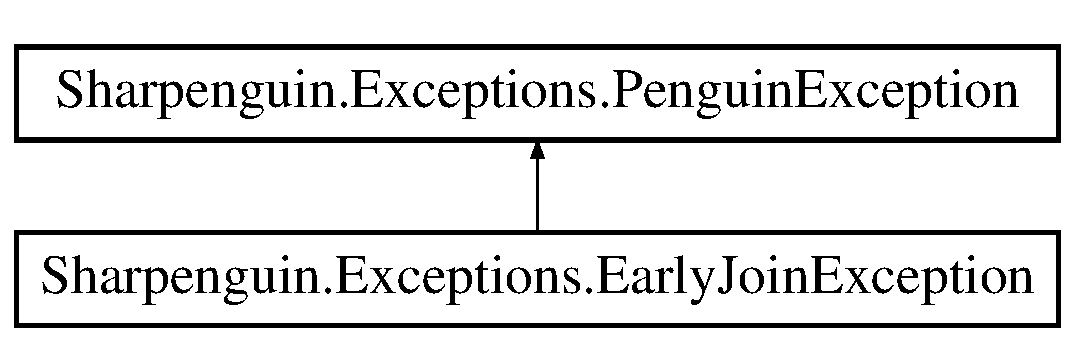
\includegraphics[height=2.000000cm]{classSharpenguin_1_1Exceptions_1_1EarlyJoinException}
\end{center}
\end{figure}
\subsection*{Public Member Functions}
\begin{DoxyCompactItemize}
\item 
\hypertarget{classSharpenguin_1_1Exceptions_1_1EarlyJoinException_a1c4b16d9df4dc74fb1a3ab63888f4384}{{\bfseries Early\-Join\-Exception} (string str\-Message)}\label{classSharpenguin_1_1Exceptions_1_1EarlyJoinException_a1c4b16d9df4dc74fb1a3ab63888f4384}

\item 
\hypertarget{classSharpenguin_1_1Exceptions_1_1EarlyJoinException_a8178db705f2d80a7512fd4a1bd14c1d8}{{\bfseries Early\-Join\-Exception} (string str\-Message, \hyperlink{classSharpenguin_1_1Exceptions_1_1EarlyJoinException}{Early\-Join\-Exception} obj\-Exception)}\label{classSharpenguin_1_1Exceptions_1_1EarlyJoinException_a8178db705f2d80a7512fd4a1bd14c1d8}

\end{DoxyCompactItemize}


\subsection{Detailed Description}
Exception for when the client tried to join a game server before login. 

The documentation for this class was generated from the following file\-:\begin{DoxyCompactItemize}
\item 
Penguin\-Exceptions.\-cs\end{DoxyCompactItemize}

\hypertarget{classSharpenguin_1_1Xt_1_1HandlerTable}{\section{\-Sharpenguin.\-Xt.\-Handler\-Table \-Class \-Reference}
\label{classSharpenguin_1_1Xt_1_1HandlerTable}\index{\-Sharpenguin.\-Xt.\-Handler\-Table@{\-Sharpenguin.\-Xt.\-Handler\-Table}}
}
\subsection*{\-Public \-Member \-Functions}
\begin{DoxyCompactItemize}
\item 
\hyperlink{classSharpenguin_1_1Xt_1_1HandlerTable_a3c993cb30c4f89943232f4416406bdd8}{\-Handler\-Table} ()
\item 
void \hyperlink{classSharpenguin_1_1Xt_1_1HandlerTable_abcd2e0f9a4786685a4a03faf7d6372b5}{\-Add} (string str\-Command, \-Packet\-Handler to\-Add)
\item 
void \hyperlink{classSharpenguin_1_1Xt_1_1HandlerTable_aab2d7871bbf5578b69994bc060a5a376}{\-Execute} (string str\-Command, \hyperlink{classSharpenguin_1_1Data_1_1PenguinPacket}{\-Data.\-Penguin\-Packet} received\-Packet)
\item 
void \hyperlink{classSharpenguin_1_1Xt_1_1HandlerTable_a6255cdc09decb3f492906d391def4de7}{\-Remove} (string str\-Command, \-Packet\-Handler to\-Remove)
\end{DoxyCompactItemize}


\subsection{\-Detailed \-Description}
\-Class to handle \hyperlink{namespaceSharpenguin_1_1Xt}{\-Xt} packets. 

\subsection{\-Constructor \& \-Destructor \-Documentation}
\hypertarget{classSharpenguin_1_1Xt_1_1HandlerTable_a3c993cb30c4f89943232f4416406bdd8}{\index{\-Sharpenguin\-::\-Xt\-::\-Handler\-Table@{\-Sharpenguin\-::\-Xt\-::\-Handler\-Table}!\-Handler\-Table@{\-Handler\-Table}}
\index{\-Handler\-Table@{\-Handler\-Table}!Sharpenguin::Xt::HandlerTable@{\-Sharpenguin\-::\-Xt\-::\-Handler\-Table}}
\subsubsection[{\-Handler\-Table}]{\setlength{\rightskip}{0pt plus 5cm}{\bf \-Sharpenguin.\-Xt.\-Handler\-Table.\-Handler\-Table} (
\begin{DoxyParamCaption}
{}
\end{DoxyParamCaption}
)\hspace{0.3cm}{\ttfamily  \mbox{[}inline\mbox{]}}}}\label{classSharpenguin_1_1Xt_1_1HandlerTable_a3c993cb30c4f89943232f4416406bdd8}
\-Handler table constructor. \-Creates the dictionary needed for storing handler delegates. 

\subsection{\-Member \-Function \-Documentation}
\hypertarget{classSharpenguin_1_1Xt_1_1HandlerTable_abcd2e0f9a4786685a4a03faf7d6372b5}{\index{\-Sharpenguin\-::\-Xt\-::\-Handler\-Table@{\-Sharpenguin\-::\-Xt\-::\-Handler\-Table}!\-Add@{\-Add}}
\index{\-Add@{\-Add}!Sharpenguin::Xt::HandlerTable@{\-Sharpenguin\-::\-Xt\-::\-Handler\-Table}}
\subsubsection[{\-Add}]{\setlength{\rightskip}{0pt plus 5cm}void {\bf \-Sharpenguin.\-Xt.\-Handler\-Table.\-Add} (
\begin{DoxyParamCaption}
\item[{string}]{str\-Command, }
\item[{\-Packet\-Handler}]{to\-Add}
\end{DoxyParamCaption}
)\hspace{0.3cm}{\ttfamily  \mbox{[}inline\mbox{]}}}}\label{classSharpenguin_1_1Xt_1_1HandlerTable_abcd2e0f9a4786685a4a03faf7d6372b5}
\-Adds a new handler.


\begin{DoxyParams}{\-Parameters}
{\em str\-Command} & \-The xt command that this handler should be registered to.\\
\hline
{\em to\-Add} & \-The delegate that the handler uses. \\
\hline
\end{DoxyParams}
\hypertarget{classSharpenguin_1_1Xt_1_1HandlerTable_aab2d7871bbf5578b69994bc060a5a376}{\index{\-Sharpenguin\-::\-Xt\-::\-Handler\-Table@{\-Sharpenguin\-::\-Xt\-::\-Handler\-Table}!\-Execute@{\-Execute}}
\index{\-Execute@{\-Execute}!Sharpenguin::Xt::HandlerTable@{\-Sharpenguin\-::\-Xt\-::\-Handler\-Table}}
\subsubsection[{\-Execute}]{\setlength{\rightskip}{0pt plus 5cm}void {\bf \-Sharpenguin.\-Xt.\-Handler\-Table.\-Execute} (
\begin{DoxyParamCaption}
\item[{string}]{str\-Command, }
\item[{{\bf \-Data.\-Penguin\-Packet}}]{received\-Packet}
\end{DoxyParamCaption}
)\hspace{0.3cm}{\ttfamily  \mbox{[}inline\mbox{]}}}}\label{classSharpenguin_1_1Xt_1_1HandlerTable_aab2d7871bbf5578b69994bc060a5a376}
\-Executes a handler by the command.


\begin{DoxyParams}{\-Parameters}
{\em str\-Command} & \-The xt command of the received packet. \\
\hline
{\em received\-Packet} & \-The packet that was received. \\
\hline
\end{DoxyParams}
\hypertarget{classSharpenguin_1_1Xt_1_1HandlerTable_a6255cdc09decb3f492906d391def4de7}{\index{\-Sharpenguin\-::\-Xt\-::\-Handler\-Table@{\-Sharpenguin\-::\-Xt\-::\-Handler\-Table}!\-Remove@{\-Remove}}
\index{\-Remove@{\-Remove}!Sharpenguin::Xt::HandlerTable@{\-Sharpenguin\-::\-Xt\-::\-Handler\-Table}}
\subsubsection[{\-Remove}]{\setlength{\rightskip}{0pt plus 5cm}void {\bf \-Sharpenguin.\-Xt.\-Handler\-Table.\-Remove} (
\begin{DoxyParamCaption}
\item[{string}]{str\-Command, }
\item[{\-Packet\-Handler}]{to\-Remove}
\end{DoxyParamCaption}
)\hspace{0.3cm}{\ttfamily  \mbox{[}inline\mbox{]}}}}\label{classSharpenguin_1_1Xt_1_1HandlerTable_a6255cdc09decb3f492906d391def4de7}
\-Removes a handler by the command.


\begin{DoxyParams}{\-Parameters}
{\em str\-Command} & \-The xt command that the handler is registered to. \\
\hline
{\em to\-Remove} & \-The delegate to remove. \\
\hline
\end{DoxyParams}


\-The documentation for this class was generated from the following file\-:\begin{DoxyCompactItemize}
\item 
\-Handler\-Table.\-cs\end{DoxyCompactItemize}

\hypertarget{classSharpenguin_1_1Exceptions_1_1InvalidAPIException}{\section{\-Sharpenguin.\-Exceptions.\-Invalid\-A\-P\-I\-Exception \-Class \-Reference}
\label{classSharpenguin_1_1Exceptions_1_1InvalidAPIException}\index{\-Sharpenguin.\-Exceptions.\-Invalid\-A\-P\-I\-Exception@{\-Sharpenguin.\-Exceptions.\-Invalid\-A\-P\-I\-Exception}}
}
\-Inheritance diagram for \-Sharpenguin.\-Exceptions.\-Invalid\-A\-P\-I\-Exception\-:\begin{figure}[H]
\begin{center}
\leavevmode
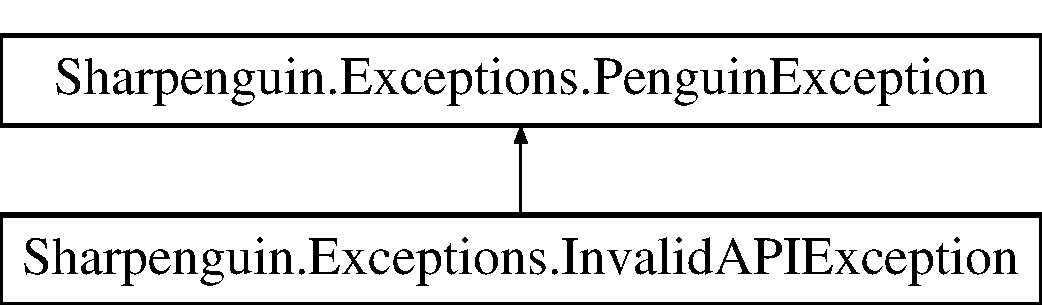
\includegraphics[height=2.000000cm]{classSharpenguin_1_1Exceptions_1_1InvalidAPIException}
\end{center}
\end{figure}
\subsection*{\-Public \-Member \-Functions}
\begin{DoxyCompactItemize}
\item 
\hypertarget{classSharpenguin_1_1Exceptions_1_1InvalidAPIException_a9f21411ded099d6ae5911a909bdec7c0}{{\bfseries \-Invalid\-A\-P\-I\-Exception} (string str\-Message)}\label{classSharpenguin_1_1Exceptions_1_1InvalidAPIException_a9f21411ded099d6ae5911a909bdec7c0}

\item 
\hypertarget{classSharpenguin_1_1Exceptions_1_1InvalidAPIException_a8e7238721e0246b07b37c6fef5a83de0}{{\bfseries \-Invalid\-A\-P\-I\-Exception} (string str\-Message, \hyperlink{classSharpenguin_1_1Exceptions_1_1InvalidAPIException}{\-Invalid\-A\-P\-I\-Exception} obj\-Exception)}\label{classSharpenguin_1_1Exceptions_1_1InvalidAPIException_a8e7238721e0246b07b37c6fef5a83de0}

\end{DoxyCompactItemize}


\subsection{\-Detailed \-Description}
\-Exception for when the server returns that the given \-A\-P\-I version is incorrect. 

\-The documentation for this class was generated from the following file\-:\begin{DoxyCompactItemize}
\item 
\-Penguin\-Exceptions.\-cs\end{DoxyCompactItemize}

\hypertarget{classSharpenguin_1_1Exceptions_1_1InvalidConfigException}{\section{\-Sharpenguin.\-Exceptions.\-Invalid\-Config\-Exception \-Class \-Reference}
\label{classSharpenguin_1_1Exceptions_1_1InvalidConfigException}\index{\-Sharpenguin.\-Exceptions.\-Invalid\-Config\-Exception@{\-Sharpenguin.\-Exceptions.\-Invalid\-Config\-Exception}}
}
\-Inheritance diagram for \-Sharpenguin.\-Exceptions.\-Invalid\-Config\-Exception\-:\begin{figure}[H]
\begin{center}
\leavevmode
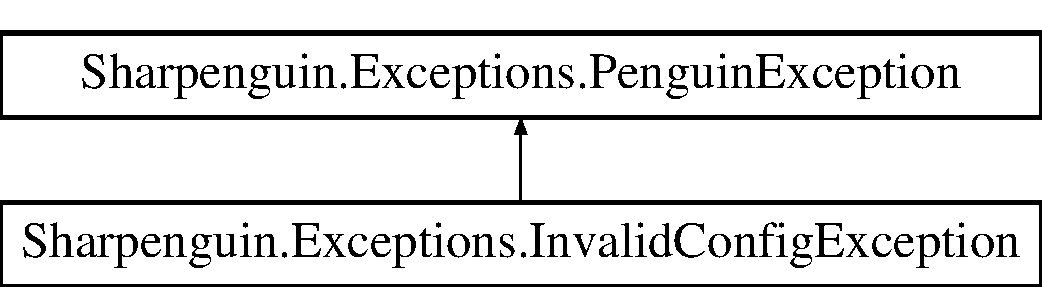
\includegraphics[height=2.000000cm]{classSharpenguin_1_1Exceptions_1_1InvalidConfigException}
\end{center}
\end{figure}
\subsection*{\-Public \-Member \-Functions}
\begin{DoxyCompactItemize}
\item 
\hypertarget{classSharpenguin_1_1Exceptions_1_1InvalidConfigException_a0c85ec92c0d3aac12be69f8cefdfed1d}{{\bfseries \-Invalid\-Config\-Exception} (string str\-Message)}\label{classSharpenguin_1_1Exceptions_1_1InvalidConfigException_a0c85ec92c0d3aac12be69f8cefdfed1d}

\item 
\hypertarget{classSharpenguin_1_1Exceptions_1_1InvalidConfigException_a74d53bab31ab1634694271b07745c83c}{{\bfseries \-Invalid\-Config\-Exception} (string str\-Message, \hyperlink{classSharpenguin_1_1Exceptions_1_1InvalidConfigException}{\-Invalid\-Config\-Exception} obj\-Exception)}\label{classSharpenguin_1_1Exceptions_1_1InvalidConfigException_a74d53bab31ab1634694271b07745c83c}

\end{DoxyCompactItemize}


\subsection{\-Detailed \-Description}
\-Exception for when the configuration file is invalid for whatever reason. 

\-The documentation for this class was generated from the following file\-:\begin{DoxyCompactItemize}
\item 
\-Penguin\-Exceptions.\-cs\end{DoxyCompactItemize}

\hypertarget{classSharpenguin_1_1Exceptions_1_1InvalidXtException}{\section{\-Sharpenguin.\-Exceptions.\-Invalid\-Xt\-Exception \-Class \-Reference}
\label{classSharpenguin_1_1Exceptions_1_1InvalidXtException}\index{\-Sharpenguin.\-Exceptions.\-Invalid\-Xt\-Exception@{\-Sharpenguin.\-Exceptions.\-Invalid\-Xt\-Exception}}
}
\-Inheritance diagram for \-Sharpenguin.\-Exceptions.\-Invalid\-Xt\-Exception\-:\begin{figure}[H]
\begin{center}
\leavevmode
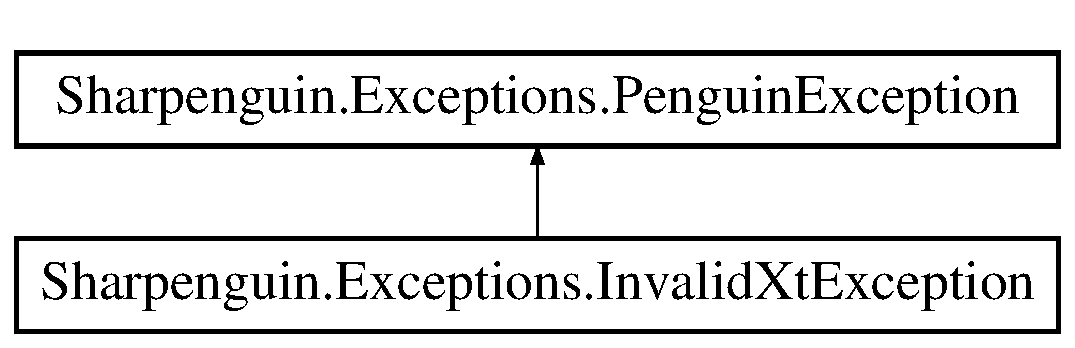
\includegraphics[height=2.000000cm]{classSharpenguin_1_1Exceptions_1_1InvalidXtException}
\end{center}
\end{figure}
\subsection*{\-Public \-Member \-Functions}
\begin{DoxyCompactItemize}
\item 
\hypertarget{classSharpenguin_1_1Exceptions_1_1InvalidXtException_ae678819fe4f70d0490f04615248f4ce4}{{\bfseries \-Invalid\-Xt\-Exception} (string str\-Message)}\label{classSharpenguin_1_1Exceptions_1_1InvalidXtException_ae678819fe4f70d0490f04615248f4ce4}

\item 
\hypertarget{classSharpenguin_1_1Exceptions_1_1InvalidXtException_ac47819418564a31ee3ccc146639c19e0}{{\bfseries \-Invalid\-Xt\-Exception} (string str\-Message, \hyperlink{classSharpenguin_1_1Exceptions_1_1InvalidXtException}{\-Invalid\-Xt\-Exception} obj\-Exception)}\label{classSharpenguin_1_1Exceptions_1_1InvalidXtException_ac47819418564a31ee3ccc146639c19e0}

\end{DoxyCompactItemize}


\subsection{\-Detailed \-Description}
\-Exception for when the \-Xt\-Parser failed to parse a string. 

\-The documentation for this class was generated from the following file\-:\begin{DoxyCompactItemize}
\item 
\-Penguin\-Exceptions.\-cs\end{DoxyCompactItemize}

\hypertarget{classProcurios_1_1Public_1_1JSON}{\section{Procurios.\-Public.\-J\-S\-O\-N Class Reference}
\label{classProcurios_1_1Public_1_1JSON}\index{Procurios.\-Public.\-J\-S\-O\-N@{Procurios.\-Public.\-J\-S\-O\-N}}
}


This class encodes and decodes \hyperlink{classProcurios_1_1Public_1_1JSON}{J\-S\-O\-N} strings. Spec. details, see \href{http://www.json.org/}{\tt http\-://www.\-json.\-org/}.  


\subsection*{Static Public Member Functions}
\begin{DoxyCompactItemize}
\item 
static object \hyperlink{classProcurios_1_1Public_1_1JSON_a8d7ead2469ab5131a06b151bb0530f4f}{Json\-Decode} (string json)
\begin{DoxyCompactList}\small\item\em Parses the string json into a value. \end{DoxyCompactList}\item 
static object \hyperlink{classProcurios_1_1Public_1_1JSON_aeb4d67c1201712a15c017611fa966e62}{Json\-Decode} (string json, ref bool success)
\begin{DoxyCompactList}\small\item\em Parses the string json into a value; and fills 'success' with the successfullness of the parse. \end{DoxyCompactList}\item 
static string \hyperlink{classProcurios_1_1Public_1_1JSON_a34ac0737167543343a0413e29aa36f12}{Json\-Encode} (object json)
\begin{DoxyCompactList}\small\item\em Converts a Hashtable / Array\-List object into a \hyperlink{classProcurios_1_1Public_1_1JSON}{J\-S\-O\-N} string. \end{DoxyCompactList}\end{DoxyCompactItemize}
\subsection*{Public Attributes}
\begin{DoxyCompactItemize}
\item 
\hypertarget{classProcurios_1_1Public_1_1JSON_af7c99e6bcc6e07c3fcceb1271f79f382}{const int {\bfseries T\-O\-K\-E\-N\-\_\-\-N\-O\-N\-E} = 0}\label{classProcurios_1_1Public_1_1JSON_af7c99e6bcc6e07c3fcceb1271f79f382}

\item 
\hypertarget{classProcurios_1_1Public_1_1JSON_aa3c331c741e9b07d0449cd3d693e1713}{const int {\bfseries T\-O\-K\-E\-N\-\_\-\-C\-U\-R\-L\-Y\-\_\-\-O\-P\-E\-N} = 1}\label{classProcurios_1_1Public_1_1JSON_aa3c331c741e9b07d0449cd3d693e1713}

\item 
\hypertarget{classProcurios_1_1Public_1_1JSON_af32234ab5b100343e0c6d09e93170ffc}{const int {\bfseries T\-O\-K\-E\-N\-\_\-\-C\-U\-R\-L\-Y\-\_\-\-C\-L\-O\-S\-E} = 2}\label{classProcurios_1_1Public_1_1JSON_af32234ab5b100343e0c6d09e93170ffc}

\item 
\hypertarget{classProcurios_1_1Public_1_1JSON_ae09402645e8eacd35ce053eafd576b61}{const int {\bfseries T\-O\-K\-E\-N\-\_\-\-S\-Q\-U\-A\-R\-E\-D\-\_\-\-O\-P\-E\-N} = 3}\label{classProcurios_1_1Public_1_1JSON_ae09402645e8eacd35ce053eafd576b61}

\item 
\hypertarget{classProcurios_1_1Public_1_1JSON_af5ab190a671a78c7174ac2605333bff3}{const int {\bfseries T\-O\-K\-E\-N\-\_\-\-S\-Q\-U\-A\-R\-E\-D\-\_\-\-C\-L\-O\-S\-E} = 4}\label{classProcurios_1_1Public_1_1JSON_af5ab190a671a78c7174ac2605333bff3}

\item 
\hypertarget{classProcurios_1_1Public_1_1JSON_ab68ed1d0266e58b25aca047c787ca03a}{const int {\bfseries T\-O\-K\-E\-N\-\_\-\-C\-O\-L\-O\-N} = 5}\label{classProcurios_1_1Public_1_1JSON_ab68ed1d0266e58b25aca047c787ca03a}

\item 
\hypertarget{classProcurios_1_1Public_1_1JSON_a7e32ab85eea665624a0495581e48e467}{const int {\bfseries T\-O\-K\-E\-N\-\_\-\-C\-O\-M\-M\-A} = 6}\label{classProcurios_1_1Public_1_1JSON_a7e32ab85eea665624a0495581e48e467}

\item 
\hypertarget{classProcurios_1_1Public_1_1JSON_a1830251b442ff565dce2f972225caee3}{const int {\bfseries T\-O\-K\-E\-N\-\_\-\-S\-T\-R\-I\-N\-G} = 7}\label{classProcurios_1_1Public_1_1JSON_a1830251b442ff565dce2f972225caee3}

\item 
\hypertarget{classProcurios_1_1Public_1_1JSON_a29f9f89bde8a04d671b7f6917d9c346e}{const int {\bfseries T\-O\-K\-E\-N\-\_\-\-N\-U\-M\-B\-E\-R} = 8}\label{classProcurios_1_1Public_1_1JSON_a29f9f89bde8a04d671b7f6917d9c346e}

\item 
\hypertarget{classProcurios_1_1Public_1_1JSON_adaf7f6f26660fb543ff4db4e9818ef4c}{const int {\bfseries T\-O\-K\-E\-N\-\_\-\-T\-R\-U\-E} = 9}\label{classProcurios_1_1Public_1_1JSON_adaf7f6f26660fb543ff4db4e9818ef4c}

\item 
\hypertarget{classProcurios_1_1Public_1_1JSON_ab2cfe0e4b9accc90f839d70459c4461b}{const int {\bfseries T\-O\-K\-E\-N\-\_\-\-F\-A\-L\-S\-E} = 10}\label{classProcurios_1_1Public_1_1JSON_ab2cfe0e4b9accc90f839d70459c4461b}

\item 
\hypertarget{classProcurios_1_1Public_1_1JSON_aa8b6fabddbbb395d62e27a0c3060955c}{const int {\bfseries T\-O\-K\-E\-N\-\_\-\-N\-U\-L\-L} = 11}\label{classProcurios_1_1Public_1_1JSON_aa8b6fabddbbb395d62e27a0c3060955c}

\end{DoxyCompactItemize}
\subsection*{Static Protected Member Functions}
\begin{DoxyCompactItemize}
\item 
\hypertarget{classProcurios_1_1Public_1_1JSON_af852c7ed4890451db945c293a379d167}{static Hashtable {\bfseries Parse\-Object} (char\mbox{[}$\,$\mbox{]} json, ref int index, ref bool success)}\label{classProcurios_1_1Public_1_1JSON_af852c7ed4890451db945c293a379d167}

\item 
\hypertarget{classProcurios_1_1Public_1_1JSON_aff252e51e51c76379df2e8b40b576d86}{static Array\-List {\bfseries Parse\-Array} (char\mbox{[}$\,$\mbox{]} json, ref int index, ref bool success)}\label{classProcurios_1_1Public_1_1JSON_aff252e51e51c76379df2e8b40b576d86}

\item 
\hypertarget{classProcurios_1_1Public_1_1JSON_a4f7e2cc33426af7ded9d103e5f23d2d2}{static object {\bfseries Parse\-Value} (char\mbox{[}$\,$\mbox{]} json, ref int index, ref bool success)}\label{classProcurios_1_1Public_1_1JSON_a4f7e2cc33426af7ded9d103e5f23d2d2}

\item 
\hypertarget{classProcurios_1_1Public_1_1JSON_a5c5148412fd6dca5b5ee9be8c941badb}{static string {\bfseries Parse\-String} (char\mbox{[}$\,$\mbox{]} json, ref int index, ref bool success)}\label{classProcurios_1_1Public_1_1JSON_a5c5148412fd6dca5b5ee9be8c941badb}

\item 
\hypertarget{classProcurios_1_1Public_1_1JSON_a9fc88d5958596687e2f0c6134ca01ff1}{static double {\bfseries Parse\-Number} (char\mbox{[}$\,$\mbox{]} json, ref int index, ref bool success)}\label{classProcurios_1_1Public_1_1JSON_a9fc88d5958596687e2f0c6134ca01ff1}

\item 
\hypertarget{classProcurios_1_1Public_1_1JSON_a462d244f6c9abc1bcfe488cc50b10fb5}{static int {\bfseries Get\-Last\-Index\-Of\-Number} (char\mbox{[}$\,$\mbox{]} json, int index)}\label{classProcurios_1_1Public_1_1JSON_a462d244f6c9abc1bcfe488cc50b10fb5}

\item 
\hypertarget{classProcurios_1_1Public_1_1JSON_a75cab5c641db9ca8275b21d3a6b891e4}{static void {\bfseries Eat\-Whitespace} (char\mbox{[}$\,$\mbox{]} json, ref int index)}\label{classProcurios_1_1Public_1_1JSON_a75cab5c641db9ca8275b21d3a6b891e4}

\item 
\hypertarget{classProcurios_1_1Public_1_1JSON_a94c3a5193fac38f9b6648404ebb6b86a}{static int {\bfseries Look\-Ahead} (char\mbox{[}$\,$\mbox{]} json, int index)}\label{classProcurios_1_1Public_1_1JSON_a94c3a5193fac38f9b6648404ebb6b86a}

\item 
\hypertarget{classProcurios_1_1Public_1_1JSON_ae3bf55097865718de308e0407aea2191}{static int {\bfseries Next\-Token} (char\mbox{[}$\,$\mbox{]} json, ref int index)}\label{classProcurios_1_1Public_1_1JSON_ae3bf55097865718de308e0407aea2191}

\item 
\hypertarget{classProcurios_1_1Public_1_1JSON_a85b20488d5e89f5d5570dcf7ff045a64}{static bool {\bfseries Serialize\-Value} (object value, String\-Builder builder)}\label{classProcurios_1_1Public_1_1JSON_a85b20488d5e89f5d5570dcf7ff045a64}

\item 
\hypertarget{classProcurios_1_1Public_1_1JSON_afcd742a1caed7b8df34868cab7faaf7e}{static bool {\bfseries Serialize\-Object} (Hashtable an\-Object, String\-Builder builder)}\label{classProcurios_1_1Public_1_1JSON_afcd742a1caed7b8df34868cab7faaf7e}

\item 
\hypertarget{classProcurios_1_1Public_1_1JSON_a720d9cc6239bc4c5b137baf947014ed6}{static bool {\bfseries Serialize\-Array} (Array\-List an\-Array, String\-Builder builder)}\label{classProcurios_1_1Public_1_1JSON_a720d9cc6239bc4c5b137baf947014ed6}

\item 
\hypertarget{classProcurios_1_1Public_1_1JSON_aac24706b51664ac548cf247cc6facdeb}{static bool {\bfseries Serialize\-String} (string a\-String, String\-Builder builder)}\label{classProcurios_1_1Public_1_1JSON_aac24706b51664ac548cf247cc6facdeb}

\item 
\hypertarget{classProcurios_1_1Public_1_1JSON_a0d383eeaab649ef0c1281132776d5630}{static bool {\bfseries Serialize\-Number} (double number, String\-Builder builder)}\label{classProcurios_1_1Public_1_1JSON_a0d383eeaab649ef0c1281132776d5630}

\end{DoxyCompactItemize}


\subsection{Detailed Description}
This class encodes and decodes \hyperlink{classProcurios_1_1Public_1_1JSON}{J\-S\-O\-N} strings. Spec. details, see \href{http://www.json.org/}{\tt http\-://www.\-json.\-org/}. 

\hyperlink{classProcurios_1_1Public_1_1JSON}{J\-S\-O\-N} uses Arrays and Objects. These correspond here to the datatypes Array\-List and Hashtable. All numbers are parsed to doubles. 

\subsection{Member Function Documentation}
\hypertarget{classProcurios_1_1Public_1_1JSON_a8d7ead2469ab5131a06b151bb0530f4f}{\index{Procurios\-::\-Public\-::\-J\-S\-O\-N@{Procurios\-::\-Public\-::\-J\-S\-O\-N}!Json\-Decode@{Json\-Decode}}
\index{Json\-Decode@{Json\-Decode}!Procurios::Public::JSON@{Procurios\-::\-Public\-::\-J\-S\-O\-N}}
\subsubsection[{Json\-Decode}]{\setlength{\rightskip}{0pt plus 5cm}static object Procurios.\-Public.\-J\-S\-O\-N.\-Json\-Decode (
\begin{DoxyParamCaption}
\item[{string}]{json}
\end{DoxyParamCaption}
)\hspace{0.3cm}{\ttfamily [inline]}, {\ttfamily [static]}}}\label{classProcurios_1_1Public_1_1JSON_a8d7ead2469ab5131a06b151bb0530f4f}


Parses the string json into a value. 


\begin{DoxyParams}{Parameters}
{\em json} & A \hyperlink{classProcurios_1_1Public_1_1JSON}{J\-S\-O\-N} string.\\
\hline
\end{DoxyParams}
\begin{DoxyReturn}{Returns}
An Array\-List, a Hashtable, a double, a string, null, true, or false
\end{DoxyReturn}
\hypertarget{classProcurios_1_1Public_1_1JSON_aeb4d67c1201712a15c017611fa966e62}{\index{Procurios\-::\-Public\-::\-J\-S\-O\-N@{Procurios\-::\-Public\-::\-J\-S\-O\-N}!Json\-Decode@{Json\-Decode}}
\index{Json\-Decode@{Json\-Decode}!Procurios::Public::JSON@{Procurios\-::\-Public\-::\-J\-S\-O\-N}}
\subsubsection[{Json\-Decode}]{\setlength{\rightskip}{0pt plus 5cm}static object Procurios.\-Public.\-J\-S\-O\-N.\-Json\-Decode (
\begin{DoxyParamCaption}
\item[{string}]{json, }
\item[{ref bool}]{success}
\end{DoxyParamCaption}
)\hspace{0.3cm}{\ttfamily [inline]}, {\ttfamily [static]}}}\label{classProcurios_1_1Public_1_1JSON_aeb4d67c1201712a15c017611fa966e62}


Parses the string json into a value; and fills 'success' with the successfullness of the parse. 


\begin{DoxyParams}{Parameters}
{\em json} & A \hyperlink{classProcurios_1_1Public_1_1JSON}{J\-S\-O\-N} string.\\
\hline
{\em success} & Successful parse?\\
\hline
\end{DoxyParams}
\begin{DoxyReturn}{Returns}
An Array\-List, a Hashtable, a double, a string, null, true, or false
\end{DoxyReturn}
\hypertarget{classProcurios_1_1Public_1_1JSON_a34ac0737167543343a0413e29aa36f12}{\index{Procurios\-::\-Public\-::\-J\-S\-O\-N@{Procurios\-::\-Public\-::\-J\-S\-O\-N}!Json\-Encode@{Json\-Encode}}
\index{Json\-Encode@{Json\-Encode}!Procurios::Public::JSON@{Procurios\-::\-Public\-::\-J\-S\-O\-N}}
\subsubsection[{Json\-Encode}]{\setlength{\rightskip}{0pt plus 5cm}static string Procurios.\-Public.\-J\-S\-O\-N.\-Json\-Encode (
\begin{DoxyParamCaption}
\item[{object}]{json}
\end{DoxyParamCaption}
)\hspace{0.3cm}{\ttfamily [inline]}, {\ttfamily [static]}}}\label{classProcurios_1_1Public_1_1JSON_a34ac0737167543343a0413e29aa36f12}


Converts a Hashtable / Array\-List object into a \hyperlink{classProcurios_1_1Public_1_1JSON}{J\-S\-O\-N} string. 


\begin{DoxyParams}{Parameters}
{\em json} & A Hashtable / Array\-List\\
\hline
\end{DoxyParams}
\begin{DoxyReturn}{Returns}
A \hyperlink{classProcurios_1_1Public_1_1JSON}{J\-S\-O\-N} encoded string, or null if object 'json' is not serializable
\end{DoxyReturn}


The documentation for this class was generated from the following file\-:\begin{DoxyCompactItemize}
\item 
J\-S\-O\-N.\-cs\end{DoxyCompactItemize}

\hypertarget{classSharpenguin_1_1Data_1_1MyPlayer}{\section{\-Sharpenguin.\-Data.\-My\-Player \-Class \-Reference}
\label{classSharpenguin_1_1Data_1_1MyPlayer}\index{\-Sharpenguin.\-Data.\-My\-Player@{\-Sharpenguin.\-Data.\-My\-Player}}
}
\-Inheritance diagram for \-Sharpenguin.\-Data.\-My\-Player\-:\begin{figure}[H]
\begin{center}
\leavevmode
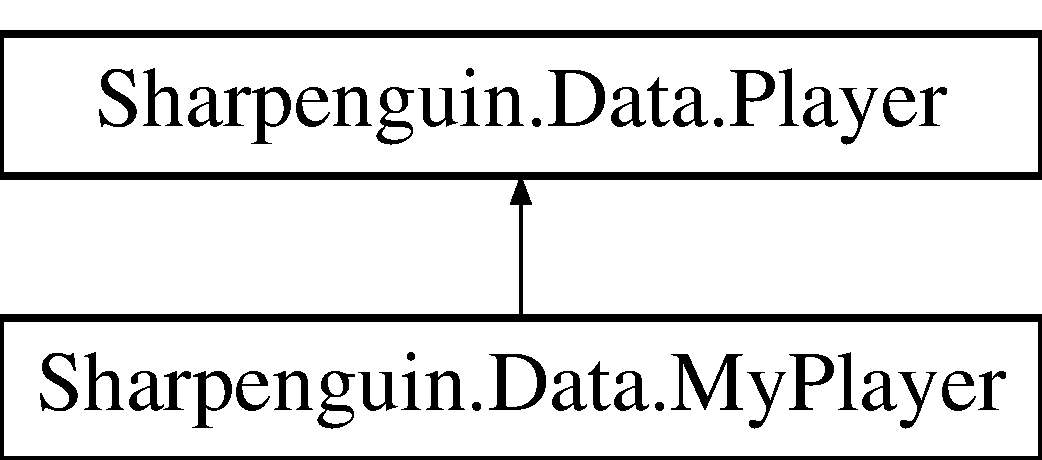
\includegraphics[height=2.000000cm]{classSharpenguin_1_1Data_1_1MyPlayer}
\end{center}
\end{figure}
\subsection*{\-Public \-Member \-Functions}
\begin{DoxyCompactItemize}
\item 
void \hyperlink{classSharpenguin_1_1Data_1_1MyPlayer_a7c6ae02df5a0ae641334476ec006a8e6}{\-Set\-Coins} (int coin\-Amount)
\item 
void \hyperlink{classSharpenguin_1_1Data_1_1MyPlayer_aeb44bb50999e60840b40332f2d0dc46b}{\-Add\-Coins} (int add\-Total)
\item 
void \hyperlink{classSharpenguin_1_1Data_1_1MyPlayer_a0fd8844c00e98e02bd7a189b04f248d2}{\-Sub\-Coins} (int sub\-Total)
\item 
void \hyperlink{classSharpenguin_1_1Data_1_1MyPlayer_a4896f30067506d8fa77f61293bed7444}{\-Set\-Age} (int total\-Days)
\item 
void \hyperlink{classSharpenguin_1_1Data_1_1MyPlayer_a84c976af85d5fb48f8137e6f047c823b}{\-Set\-Member\-Remaining} (int total\-Days)
\item 
void \hyperlink{classSharpenguin_1_1Data_1_1MyPlayer_a9e96ff952268372d8b43cbde269b58d5}{\-Set\-Minutes\-Played} (int total\-Minutes)
\item 
void \hyperlink{classSharpenguin_1_1Data_1_1MyPlayer_ad9bf7d1039275986d48cb2c0c11144ac}{\-Add\-Inventory\-Item} (int item\-Id)
\end{DoxyCompactItemize}
\subsection*{\-Properties}
\begin{DoxyCompactItemize}
\item 
\hypertarget{classSharpenguin_1_1Data_1_1MyPlayer_ae78b8a9ecf05afedb7baed1336e82dee}{int {\bfseries \-Age}\hspace{0.3cm}{\ttfamily  \mbox{[}get\mbox{]}}}\label{classSharpenguin_1_1Data_1_1MyPlayer_ae78b8a9ecf05afedb7baed1336e82dee}

\item 
\hypertarget{classSharpenguin_1_1Data_1_1MyPlayer_a3f6ac8fc09a165c81a23d25ff016b7e2}{int {\bfseries \-Coins}\hspace{0.3cm}{\ttfamily  \mbox{[}get\mbox{]}}}\label{classSharpenguin_1_1Data_1_1MyPlayer_a3f6ac8fc09a165c81a23d25ff016b7e2}

\item 
\hypertarget{classSharpenguin_1_1Data_1_1MyPlayer_acffca37897a5d514aba1eb8156b67813}{int {\bfseries \-Member\-Remaining}\hspace{0.3cm}{\ttfamily  \mbox{[}get\mbox{]}}}\label{classSharpenguin_1_1Data_1_1MyPlayer_acffca37897a5d514aba1eb8156b67813}

\item 
\hypertarget{classSharpenguin_1_1Data_1_1MyPlayer_aa706275c546c3c0d4dddb6e2258ab3a4}{int {\bfseries \-Minutes\-Played}\hspace{0.3cm}{\ttfamily  \mbox{[}get\mbox{]}}}\label{classSharpenguin_1_1Data_1_1MyPlayer_aa706275c546c3c0d4dddb6e2258ab3a4}

\item 
\hypertarget{classSharpenguin_1_1Data_1_1MyPlayer_ae25dc7ef58b29f12bceb53e1706141fe}{int\mbox{[}$\,$\mbox{]} {\bfseries \-Inventory}\hspace{0.3cm}{\ttfamily  \mbox{[}get\mbox{]}}}\label{classSharpenguin_1_1Data_1_1MyPlayer_ae25dc7ef58b29f12bceb53e1706141fe}

\end{DoxyCompactItemize}


\subsection{\-Detailed \-Description}
\-An extension class of player for your own player. 

\subsection{\-Member \-Function \-Documentation}
\hypertarget{classSharpenguin_1_1Data_1_1MyPlayer_aeb44bb50999e60840b40332f2d0dc46b}{\index{\-Sharpenguin\-::\-Data\-::\-My\-Player@{\-Sharpenguin\-::\-Data\-::\-My\-Player}!\-Add\-Coins@{\-Add\-Coins}}
\index{\-Add\-Coins@{\-Add\-Coins}!Sharpenguin::Data::MyPlayer@{\-Sharpenguin\-::\-Data\-::\-My\-Player}}
\subsubsection[{\-Add\-Coins}]{\setlength{\rightskip}{0pt plus 5cm}void {\bf \-Sharpenguin.\-Data.\-My\-Player.\-Add\-Coins} (
\begin{DoxyParamCaption}
\item[{int}]{add\-Total}
\end{DoxyParamCaption}
)\hspace{0.3cm}{\ttfamily  \mbox{[}inline\mbox{]}}}}\label{classSharpenguin_1_1Data_1_1MyPlayer_aeb44bb50999e60840b40332f2d0dc46b}
\-Adds coins to the total coin amount.


\begin{DoxyParams}{\-Parameters}
{\em add\-Total} & \-The amount of coins to add. \\
\hline
\end{DoxyParams}
\hypertarget{classSharpenguin_1_1Data_1_1MyPlayer_ad9bf7d1039275986d48cb2c0c11144ac}{\index{\-Sharpenguin\-::\-Data\-::\-My\-Player@{\-Sharpenguin\-::\-Data\-::\-My\-Player}!\-Add\-Inventory\-Item@{\-Add\-Inventory\-Item}}
\index{\-Add\-Inventory\-Item@{\-Add\-Inventory\-Item}!Sharpenguin::Data::MyPlayer@{\-Sharpenguin\-::\-Data\-::\-My\-Player}}
\subsubsection[{\-Add\-Inventory\-Item}]{\setlength{\rightskip}{0pt plus 5cm}void {\bf \-Sharpenguin.\-Data.\-My\-Player.\-Add\-Inventory\-Item} (
\begin{DoxyParamCaption}
\item[{int}]{item\-Id}
\end{DoxyParamCaption}
)\hspace{0.3cm}{\ttfamily  \mbox{[}inline\mbox{]}}}}\label{classSharpenguin_1_1Data_1_1MyPlayer_ad9bf7d1039275986d48cb2c0c11144ac}
\-Adds an item to the inventory list.


\begin{DoxyParams}{\-Parameters}
{\em item\-Id} & \-The id of the item to add. \\
\hline
\end{DoxyParams}
\hypertarget{classSharpenguin_1_1Data_1_1MyPlayer_a4896f30067506d8fa77f61293bed7444}{\index{\-Sharpenguin\-::\-Data\-::\-My\-Player@{\-Sharpenguin\-::\-Data\-::\-My\-Player}!\-Set\-Age@{\-Set\-Age}}
\index{\-Set\-Age@{\-Set\-Age}!Sharpenguin::Data::MyPlayer@{\-Sharpenguin\-::\-Data\-::\-My\-Player}}
\subsubsection[{\-Set\-Age}]{\setlength{\rightskip}{0pt plus 5cm}void {\bf \-Sharpenguin.\-Data.\-My\-Player.\-Set\-Age} (
\begin{DoxyParamCaption}
\item[{int}]{total\-Days}
\end{DoxyParamCaption}
)\hspace{0.3cm}{\ttfamily  \mbox{[}inline\mbox{]}}}}\label{classSharpenguin_1_1Data_1_1MyPlayer_a4896f30067506d8fa77f61293bed7444}
\-Sets the age of the player.


\begin{DoxyParams}{\-Parameters}
{\em total\-Days} & \-How many days old the player is. \\
\hline
\end{DoxyParams}
\hypertarget{classSharpenguin_1_1Data_1_1MyPlayer_a7c6ae02df5a0ae641334476ec006a8e6}{\index{\-Sharpenguin\-::\-Data\-::\-My\-Player@{\-Sharpenguin\-::\-Data\-::\-My\-Player}!\-Set\-Coins@{\-Set\-Coins}}
\index{\-Set\-Coins@{\-Set\-Coins}!Sharpenguin::Data::MyPlayer@{\-Sharpenguin\-::\-Data\-::\-My\-Player}}
\subsubsection[{\-Set\-Coins}]{\setlength{\rightskip}{0pt plus 5cm}void {\bf \-Sharpenguin.\-Data.\-My\-Player.\-Set\-Coins} (
\begin{DoxyParamCaption}
\item[{int}]{coin\-Amount}
\end{DoxyParamCaption}
)\hspace{0.3cm}{\ttfamily  \mbox{[}inline\mbox{]}}}}\label{classSharpenguin_1_1Data_1_1MyPlayer_a7c6ae02df5a0ae641334476ec006a8e6}
\-Sets how many coins the player has.


\begin{DoxyParams}{\-Parameters}
{\em coin\-Amount} & \-The amount of coins that the player has. \\
\hline
\end{DoxyParams}
\hypertarget{classSharpenguin_1_1Data_1_1MyPlayer_a84c976af85d5fb48f8137e6f047c823b}{\index{\-Sharpenguin\-::\-Data\-::\-My\-Player@{\-Sharpenguin\-::\-Data\-::\-My\-Player}!\-Set\-Member\-Remaining@{\-Set\-Member\-Remaining}}
\index{\-Set\-Member\-Remaining@{\-Set\-Member\-Remaining}!Sharpenguin::Data::MyPlayer@{\-Sharpenguin\-::\-Data\-::\-My\-Player}}
\subsubsection[{\-Set\-Member\-Remaining}]{\setlength{\rightskip}{0pt plus 5cm}void {\bf \-Sharpenguin.\-Data.\-My\-Player.\-Set\-Member\-Remaining} (
\begin{DoxyParamCaption}
\item[{int}]{total\-Days}
\end{DoxyParamCaption}
)\hspace{0.3cm}{\ttfamily  \mbox{[}inline\mbox{]}}}}\label{classSharpenguin_1_1Data_1_1MyPlayer_a84c976af85d5fb48f8137e6f047c823b}
\-Sets the remaining member days that the player has.


\begin{DoxyParams}{\-Parameters}
{\em total\-Days} & \-The amount of days remaining. \\
\hline
\end{DoxyParams}
\hypertarget{classSharpenguin_1_1Data_1_1MyPlayer_a9e96ff952268372d8b43cbde269b58d5}{\index{\-Sharpenguin\-::\-Data\-::\-My\-Player@{\-Sharpenguin\-::\-Data\-::\-My\-Player}!\-Set\-Minutes\-Played@{\-Set\-Minutes\-Played}}
\index{\-Set\-Minutes\-Played@{\-Set\-Minutes\-Played}!Sharpenguin::Data::MyPlayer@{\-Sharpenguin\-::\-Data\-::\-My\-Player}}
\subsubsection[{\-Set\-Minutes\-Played}]{\setlength{\rightskip}{0pt plus 5cm}void {\bf \-Sharpenguin.\-Data.\-My\-Player.\-Set\-Minutes\-Played} (
\begin{DoxyParamCaption}
\item[{int}]{total\-Minutes}
\end{DoxyParamCaption}
)\hspace{0.3cm}{\ttfamily  \mbox{[}inline\mbox{]}}}}\label{classSharpenguin_1_1Data_1_1MyPlayer_a9e96ff952268372d8b43cbde269b58d5}
\-Sets the amount of minutes that the player has played the game.


\begin{DoxyParams}{\-Parameters}
{\em total\-Minutes} & \-The total amount of minutes that the player has played. \\
\hline
\end{DoxyParams}
\hypertarget{classSharpenguin_1_1Data_1_1MyPlayer_a0fd8844c00e98e02bd7a189b04f248d2}{\index{\-Sharpenguin\-::\-Data\-::\-My\-Player@{\-Sharpenguin\-::\-Data\-::\-My\-Player}!\-Sub\-Coins@{\-Sub\-Coins}}
\index{\-Sub\-Coins@{\-Sub\-Coins}!Sharpenguin::Data::MyPlayer@{\-Sharpenguin\-::\-Data\-::\-My\-Player}}
\subsubsection[{\-Sub\-Coins}]{\setlength{\rightskip}{0pt plus 5cm}void {\bf \-Sharpenguin.\-Data.\-My\-Player.\-Sub\-Coins} (
\begin{DoxyParamCaption}
\item[{int}]{sub\-Total}
\end{DoxyParamCaption}
)\hspace{0.3cm}{\ttfamily  \mbox{[}inline\mbox{]}}}}\label{classSharpenguin_1_1Data_1_1MyPlayer_a0fd8844c00e98e02bd7a189b04f248d2}
\-Subtracts coins from the total coin amount. 
\begin{DoxyParams}{\-Parameters}
{\em sub\-Total} & \-The amount of coins to subtract. \\
\hline
\end{DoxyParams}


\-The documentation for this class was generated from the following file\-:\begin{DoxyCompactItemize}
\item 
\-My\-Player.\-cs\end{DoxyCompactItemize}

\hypertarget{classSharpenguin_1_1Exceptions_1_1NonExistantCrumbException}{\section{\-Sharpenguin.\-Exceptions.\-Non\-Existant\-Crumb\-Exception \-Class \-Reference}
\label{classSharpenguin_1_1Exceptions_1_1NonExistantCrumbException}\index{\-Sharpenguin.\-Exceptions.\-Non\-Existant\-Crumb\-Exception@{\-Sharpenguin.\-Exceptions.\-Non\-Existant\-Crumb\-Exception}}
}
\-Inheritance diagram for \-Sharpenguin.\-Exceptions.\-Non\-Existant\-Crumb\-Exception\-:\begin{figure}[H]
\begin{center}
\leavevmode
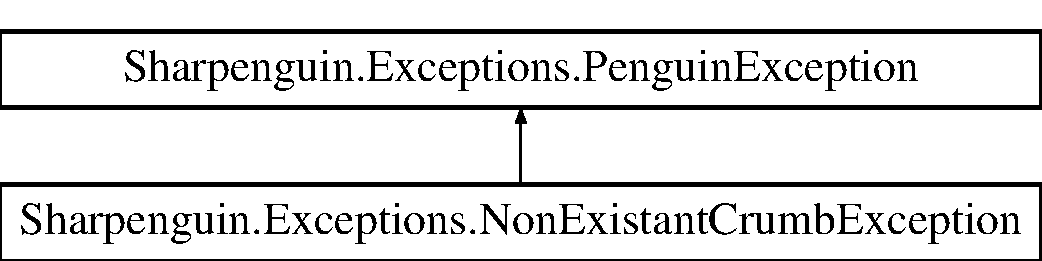
\includegraphics[height=2.000000cm]{classSharpenguin_1_1Exceptions_1_1NonExistantCrumbException}
\end{center}
\end{figure}
\subsection*{\-Public \-Member \-Functions}
\begin{DoxyCompactItemize}
\item 
\hypertarget{classSharpenguin_1_1Exceptions_1_1NonExistantCrumbException_af8bda657fe2945c89dafe8f0c5cce170}{{\bfseries \-Non\-Existant\-Crumb\-Exception} (string str\-Message)}\label{classSharpenguin_1_1Exceptions_1_1NonExistantCrumbException_af8bda657fe2945c89dafe8f0c5cce170}

\item 
\hypertarget{classSharpenguin_1_1Exceptions_1_1NonExistantCrumbException_a39ea74af873c1a57483b7a5062be9e8d}{{\bfseries \-Non\-Existant\-Crumb\-Exception} (string str\-Message, \hyperlink{classSharpenguin_1_1Exceptions_1_1NonExistantCrumbException}{\-Non\-Existant\-Crumb\-Exception} obj\-Exception)}\label{classSharpenguin_1_1Exceptions_1_1NonExistantCrumbException_a39ea74af873c1a57483b7a5062be9e8d}

\end{DoxyCompactItemize}


\subsection{\-Detailed \-Description}
\-Exception for when a crumb which does not exist was attempted to be accessed. 

\-The documentation for this class was generated from the following file\-:\begin{DoxyCompactItemize}
\item 
\-Penguin\-Exceptions.\-cs\end{DoxyCompactItemize}

\hypertarget{classSharpenguin_1_1Exceptions_1_1NonExistantPlayerException}{\section{Sharpenguin.\-Exceptions.\-Non\-Existant\-Player\-Exception Class Reference}
\label{classSharpenguin_1_1Exceptions_1_1NonExistantPlayerException}\index{Sharpenguin.\-Exceptions.\-Non\-Existant\-Player\-Exception@{Sharpenguin.\-Exceptions.\-Non\-Existant\-Player\-Exception}}
}
Inheritance diagram for Sharpenguin.\-Exceptions.\-Non\-Existant\-Player\-Exception\-:\begin{figure}[H]
\begin{center}
\leavevmode
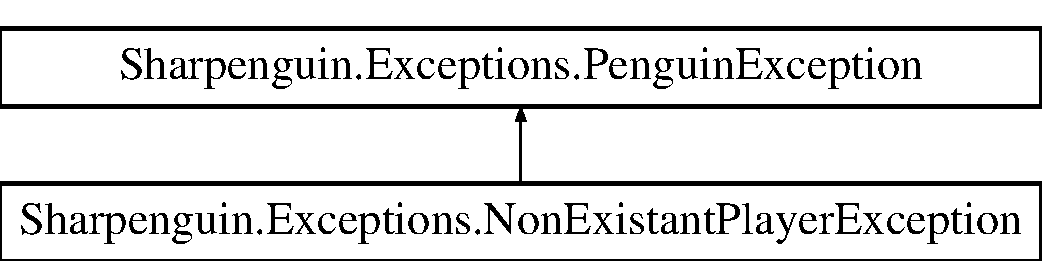
\includegraphics[height=2.000000cm]{classSharpenguin_1_1Exceptions_1_1NonExistantPlayerException}
\end{center}
\end{figure}
\subsection*{Public Member Functions}
\begin{DoxyCompactItemize}
\item 
\hypertarget{classSharpenguin_1_1Exceptions_1_1NonExistantPlayerException_a90511b21814b1bc2db9d2fdb1fe9aca5}{{\bfseries Non\-Existant\-Player\-Exception} (string str\-Message)}\label{classSharpenguin_1_1Exceptions_1_1NonExistantPlayerException_a90511b21814b1bc2db9d2fdb1fe9aca5}

\item 
\hypertarget{classSharpenguin_1_1Exceptions_1_1NonExistantPlayerException_a4e058a758643f7834239e6a76225afec}{{\bfseries Non\-Existant\-Player\-Exception} (string str\-Message, \hyperlink{classSharpenguin_1_1Exceptions_1_1NonExistantPlayerException}{Non\-Existant\-Player\-Exception} obj\-Exception)}\label{classSharpenguin_1_1Exceptions_1_1NonExistantPlayerException_a4e058a758643f7834239e6a76225afec}

\end{DoxyCompactItemize}


\subsection{Detailed Description}
Exception for when a player is not in the room, but the client tried to get their player object. 

The documentation for this class was generated from the following file\-:\begin{DoxyCompactItemize}
\item 
Penguin\-Exceptions.\-cs\end{DoxyCompactItemize}

\hypertarget{classSharpenguin_1_1Penguin}{\section{Sharpenguin.\-Penguin Class Reference}
\label{classSharpenguin_1_1Penguin}\index{Sharpenguin.\-Penguin@{Sharpenguin.\-Penguin}}
}
Inheritance diagram for Sharpenguin.\-Penguin\-:\begin{figure}[H]
\begin{center}
\leavevmode
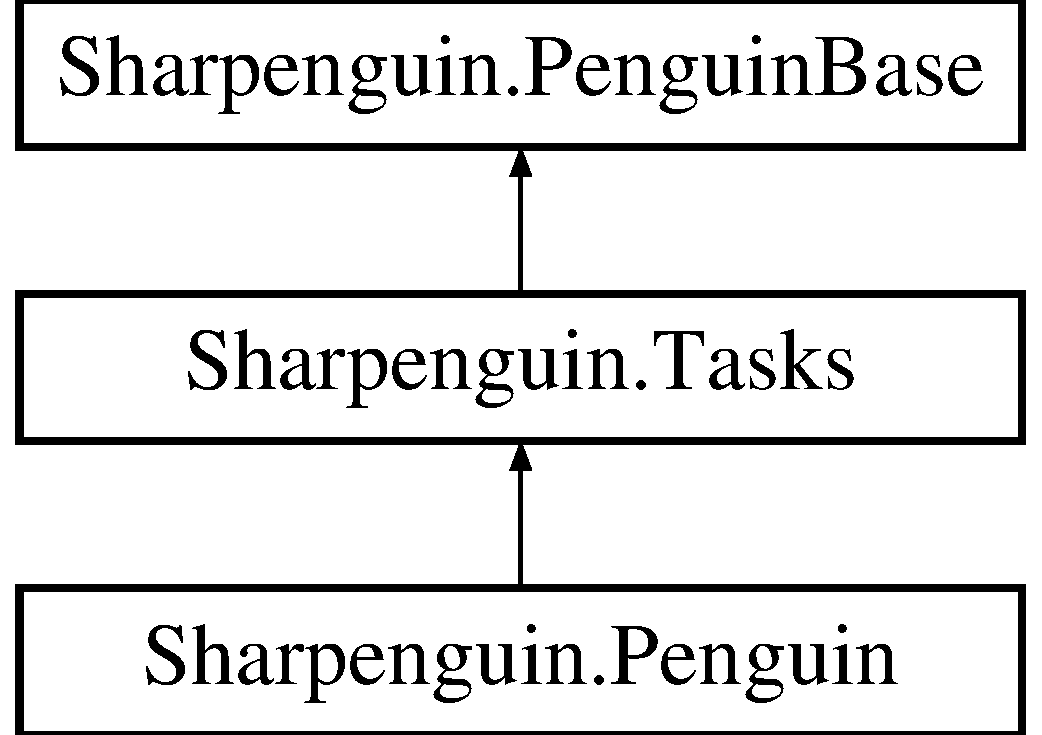
\includegraphics[height=3.000000cm]{classSharpenguin_1_1Penguin}
\end{center}
\end{figure}
\subsection*{Public Member Functions}
\begin{DoxyCompactItemize}
\item 
\hyperlink{classSharpenguin_1_1Penguin_a1ee6c5297d0f6dad402b209929cf6ca7}{Penguin} ()
\item 
void \hyperlink{classSharpenguin_1_1Penguin_af2f456a088666e640eb56afdd58f25a6}{Handle\-Inventory\-List} (\hyperlink{classSharpenguin_1_1Data_1_1PenguinPacket}{Data.\-Penguin\-Packet} received\-Packet)
\end{DoxyCompactItemize}


\subsection{Constructor \& Destructor Documentation}
\hypertarget{classSharpenguin_1_1Penguin_a1ee6c5297d0f6dad402b209929cf6ca7}{\index{Sharpenguin\-::\-Penguin@{Sharpenguin\-::\-Penguin}!Penguin@{Penguin}}
\index{Penguin@{Penguin}!Sharpenguin::Penguin@{Sharpenguin\-::\-Penguin}}
\subsubsection[{Penguin}]{\setlength{\rightskip}{0pt plus 5cm}Sharpenguin.\-Penguin.\-Penguin (
\begin{DoxyParamCaption}
{}
\end{DoxyParamCaption}
)\hspace{0.3cm}{\ttfamily [inline]}}}\label{classSharpenguin_1_1Penguin_a1ee6c5297d0f6dad402b209929cf6ca7}
\hyperlink{classSharpenguin_1_1Penguin}{Penguin} construct. Starts the loading of the system handlers. 

\subsection{Member Function Documentation}
\hypertarget{classSharpenguin_1_1Penguin_af2f456a088666e640eb56afdd58f25a6}{\index{Sharpenguin\-::\-Penguin@{Sharpenguin\-::\-Penguin}!Handle\-Inventory\-List@{Handle\-Inventory\-List}}
\index{Handle\-Inventory\-List@{Handle\-Inventory\-List}!Sharpenguin::Penguin@{Sharpenguin\-::\-Penguin}}
\subsubsection[{Handle\-Inventory\-List}]{\setlength{\rightskip}{0pt plus 5cm}void Sharpenguin.\-Penguin.\-Handle\-Inventory\-List (
\begin{DoxyParamCaption}
\item[{{\bf Data.\-Penguin\-Packet}}]{received\-Packet}
\end{DoxyParamCaption}
)\hspace{0.3cm}{\ttfamily [inline]}}}\label{classSharpenguin_1_1Penguin_af2f456a088666e640eb56afdd58f25a6}
Handles the inventory list packet, (handler \char`\"{}gi\char`\"{}).


\begin{DoxyParams}{Parameters}
{\em received\-Packet} & The packet to handle. \\
\hline
\end{DoxyParams}


The documentation for this class was generated from the following file\-:\begin{DoxyCompactItemize}
\item 
Penguin.\-cs\end{DoxyCompactItemize}

\hypertarget{classSharpenguin_1_1PenguinBase}{\section{Sharpenguin.\-Penguin\-Base Class Reference}
\label{classSharpenguin_1_1PenguinBase}\index{Sharpenguin.\-Penguin\-Base@{Sharpenguin.\-Penguin\-Base}}
}
Inheritance diagram for Sharpenguin.\-Penguin\-Base\-:\begin{figure}[H]
\begin{center}
\leavevmode
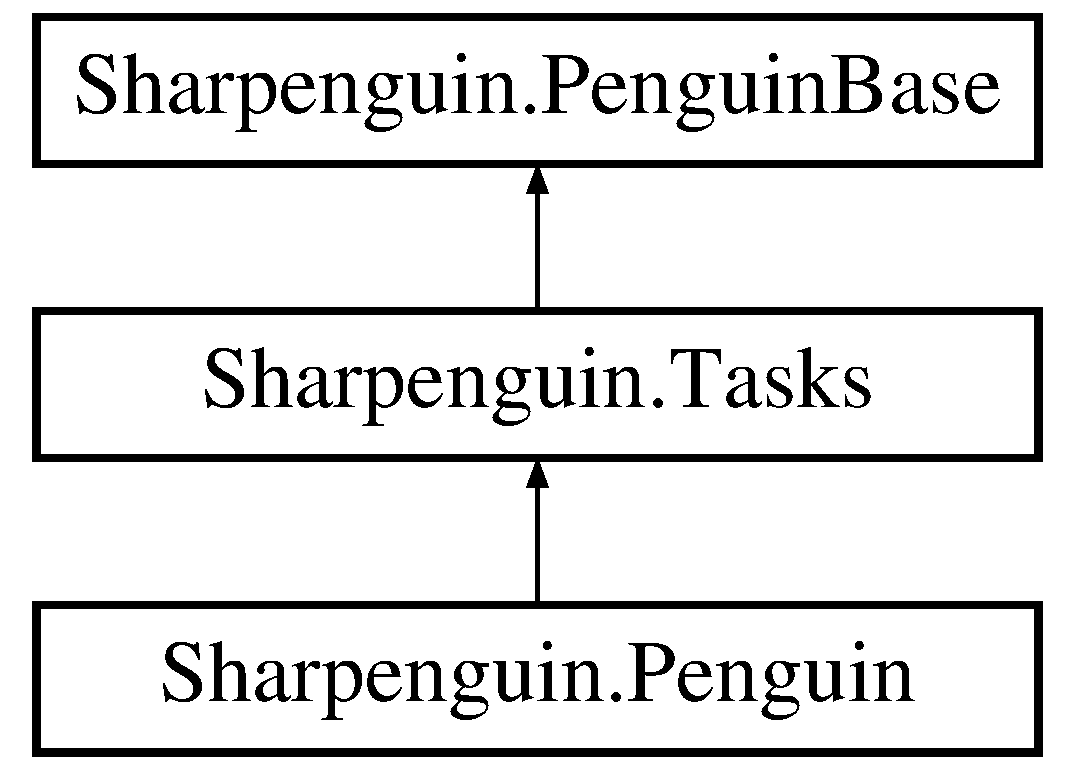
\includegraphics[height=3.000000cm]{classSharpenguin_1_1PenguinBase}
\end{center}
\end{figure}
\subsection*{Public Member Functions}
\begin{DoxyCompactItemize}
\item 
\hyperlink{classSharpenguin_1_1PenguinBase_abae69c0be10d8de6f6f852a5a9820c44}{Penguin\-Base} ()
\item 
void \hyperlink{classSharpenguin_1_1PenguinBase_a339081cc6d7b689525639e9c41275d53}{Login} (string str\-Username, string str\-Password)
\item 
void \hyperlink{classSharpenguin_1_1PenguinBase_ae883a098b18a513c9ca47e80d833c32e}{Join} (object obj\-Server)
\item 
void \hyperlink{classSharpenguin_1_1PenguinBase_a50ba7c1e17673282b539e280c4552773}{Send\-Data} (string str\-Data)
\item 
void \hyperlink{classSharpenguin_1_1PenguinBase_a1c56da96688962cc6db870fad34b9e62}{Disconnect} ()
\end{DoxyCompactItemize}
\subsection*{Protected Member Functions}
\begin{DoxyCompactItemize}
\item 
void \hyperlink{classSharpenguin_1_1PenguinBase_aa6a126810f26f0b1d85b8c6e35eed5c9}{Login\-Finished} ()
\item 
void \hyperlink{classSharpenguin_1_1PenguinBase_a64a4a3cd550fd49156f9ed5fbd1836ed}{Join\-Finished} ()
\item 
void \hyperlink{classSharpenguin_1_1PenguinBase_a0d866e6fe167c36721fc282cb36d9d07}{Receive\-Callback} (\hyperlink{classSharpenguin_1_1Data_1_1PenguinPacket}{Data.\-Penguin\-Packet} received\-Packet)
\item 
void \hyperlink{classSharpenguin_1_1PenguinBase_a06facd0f0f753fa79596ae31a6811a86}{Disconnect\-Callback} ()
\end{DoxyCompactItemize}
\subsection*{Protected Attributes}
\begin{DoxyCompactItemize}
\item 
\hypertarget{classSharpenguin_1_1PenguinBase_a3040b77fea34fa80159705a8f610783c}{\hyperlink{classSharpenguin_1_1Data_1_1PenguinRoom}{Data.\-Penguin\-Room} {\bfseries current\-Room}}\label{classSharpenguin_1_1PenguinBase_a3040b77fea34fa80159705a8f610783c}

\item 
\hypertarget{classSharpenguin_1_1PenguinBase_ab30aeba363ab0c00583924dce54bf6ba}{int {\bfseries ext\-Room\-I\-D}}\label{classSharpenguin_1_1PenguinBase_ab30aeba363ab0c00583924dce54bf6ba}

\item 
\hypertarget{classSharpenguin_1_1PenguinBase_a7e8cc4749d5b1f56fec1cfed440bdfec}{int {\bfseries int\-Player\-I\-D}}\label{classSharpenguin_1_1PenguinBase_a7e8cc4749d5b1f56fec1cfed440bdfec}

\item 
\hypertarget{classSharpenguin_1_1PenguinBase_a8a73235e69c6ee95ab525449f91a7d04}{int {\bfseries int\-Room\-I\-D} = -\/1}\label{classSharpenguin_1_1PenguinBase_a8a73235e69c6ee95ab525449f91a7d04}

\item 
\hypertarget{classSharpenguin_1_1PenguinBase_ad35590cd769800ad5534cb53f5bf044a}{bool {\bfseries bln\-Is\-Login} = false}\label{classSharpenguin_1_1PenguinBase_ad35590cd769800ad5534cb53f5bf044a}

\item 
\hypertarget{classSharpenguin_1_1PenguinBase_ae8d83319d81662d7d133f1f7ead386a9}{bool {\bfseries bln\-Is\-Join} = false}\label{classSharpenguin_1_1PenguinBase_ae8d83319d81662d7d133f1f7ead386a9}

\item 
\hypertarget{classSharpenguin_1_1PenguinBase_a16671246037e50e34685781ff82da687}{string {\bfseries str\-Username} = \char`\"{}\char`\"{}}\label{classSharpenguin_1_1PenguinBase_a16671246037e50e34685781ff82da687}

\item 
\hypertarget{classSharpenguin_1_1PenguinBase_a4ebef7c32b60971bdf6e17dbf911b96c}{string {\bfseries str\-Password} = \char`\"{}\char`\"{}}\label{classSharpenguin_1_1PenguinBase_a4ebef7c32b60971bdf6e17dbf911b96c}

\item 
\hypertarget{classSharpenguin_1_1PenguinBase_ae4232fad4dad9b1118a2227dc1a85b9f}{string {\bfseries str\-Login\-Key} = \char`\"{}\char`\"{}}\label{classSharpenguin_1_1PenguinBase_ae4232fad4dad9b1118a2227dc1a85b9f}

\item 
\hypertarget{classSharpenguin_1_1PenguinBase_a96f07f160ff42b6a544545394f7058c5}{string {\bfseries str\-Rnd\-K} = \char`\"{}\char`\"{}}\label{classSharpenguin_1_1PenguinBase_a96f07f160ff42b6a544545394f7058c5}

\item 
\hypertarget{classSharpenguin_1_1PenguinBase_a081570b66c694bab1df58a083e34ef4a}{Error\-Handler {\bfseries penguin\-Error\-Event}}\label{classSharpenguin_1_1PenguinBase_a081570b66c694bab1df58a083e34ef4a}

\end{DoxyCompactItemize}
\subsection*{Properties}
\begin{DoxyCompactItemize}
\item 
\hypertarget{classSharpenguin_1_1PenguinBase_aae21196fbe688005b7a0d0a0b8bf42ed}{int \hyperlink{classSharpenguin_1_1PenguinBase_aae21196fbe688005b7a0d0a0b8bf42ed}{I\-D}\hspace{0.3cm}{\ttfamily  \mbox{[}get\mbox{]}}}\label{classSharpenguin_1_1PenguinBase_aae21196fbe688005b7a0d0a0b8bf42ed}

\begin{DoxyCompactList}\small\item\em Get's your I\-D. \end{DoxyCompactList}\item 
\hypertarget{classSharpenguin_1_1PenguinBase_a0d4aa128eef283472312ce191841887a}{int \hyperlink{classSharpenguin_1_1PenguinBase_a0d4aa128eef283472312ce191841887a}{Int\-Room}\hspace{0.3cm}{\ttfamily  \mbox{[}get\mbox{]}}}\label{classSharpenguin_1_1PenguinBase_a0d4aa128eef283472312ce191841887a}

\begin{DoxyCompactList}\small\item\em Gets your internal room I\-D. \end{DoxyCompactList}\item 
\hypertarget{classSharpenguin_1_1PenguinBase_ae290be3f9aa1e9f5d474cde01a3bb2ac}{int \hyperlink{classSharpenguin_1_1PenguinBase_ae290be3f9aa1e9f5d474cde01a3bb2ac}{Ext\-Room}\hspace{0.3cm}{\ttfamily  \mbox{[}get\mbox{]}}}\label{classSharpenguin_1_1PenguinBase_ae290be3f9aa1e9f5d474cde01a3bb2ac}

\begin{DoxyCompactList}\small\item\em Gets your external room I\-D. \end{DoxyCompactList}\item 
\hypertarget{classSharpenguin_1_1PenguinBase_af52eaa01201024b8c065f53e85120d12}{string \hyperlink{classSharpenguin_1_1PenguinBase_af52eaa01201024b8c065f53e85120d12}{Username}\hspace{0.3cm}{\ttfamily  \mbox{[}get\mbox{]}}}\label{classSharpenguin_1_1PenguinBase_af52eaa01201024b8c065f53e85120d12}

\begin{DoxyCompactList}\small\item\em Gets your username. \end{DoxyCompactList}\item 
\hypertarget{classSharpenguin_1_1PenguinBase_a370b4ae2070f96b55fbef267d4d6b27e}{Login\-Handler \hyperlink{classSharpenguin_1_1PenguinBase_a370b4ae2070f96b55fbef267d4d6b27e}{on\-Login}\hspace{0.3cm}{\ttfamily  \mbox{[}get, set\mbox{]}}}\label{classSharpenguin_1_1PenguinBase_a370b4ae2070f96b55fbef267d4d6b27e}

\begin{DoxyCompactList}\small\item\em Event called after login success. \end{DoxyCompactList}\item 
\hypertarget{classSharpenguin_1_1PenguinBase_a671a22a751f91b472db6f427c618c131}{Join\-Handler \hyperlink{classSharpenguin_1_1PenguinBase_a671a22a751f91b472db6f427c618c131}{on\-Join}\hspace{0.3cm}{\ttfamily  \mbox{[}get, set\mbox{]}}}\label{classSharpenguin_1_1PenguinBase_a671a22a751f91b472db6f427c618c131}

\begin{DoxyCompactList}\small\item\em Event called when the penguin has joined the game server. \end{DoxyCompactList}\item 
\hypertarget{classSharpenguin_1_1PenguinBase_ac2b810a66bab0069126d07ebe0ccfa42}{Packet\-Handler \hyperlink{classSharpenguin_1_1PenguinBase_ac2b810a66bab0069126d07ebe0ccfa42}{on\-Receive}\hspace{0.3cm}{\ttfamily  \mbox{[}get, set\mbox{]}}}\label{classSharpenguin_1_1PenguinBase_ac2b810a66bab0069126d07ebe0ccfa42}

\begin{DoxyCompactList}\small\item\em Event called when we have received a packet from the server. \end{DoxyCompactList}\item 
\hypertarget{classSharpenguin_1_1PenguinBase_a11a9cb86a237e4aff2903c84cbc0d26f}{Disconnect\-Handler \hyperlink{classSharpenguin_1_1PenguinBase_a11a9cb86a237e4aff2903c84cbc0d26f}{on\-Disconnect}\hspace{0.3cm}{\ttfamily  \mbox{[}get, set\mbox{]}}}\label{classSharpenguin_1_1PenguinBase_a11a9cb86a237e4aff2903c84cbc0d26f}

\begin{DoxyCompactList}\small\item\em Event called when we have disconnected from the server. \end{DoxyCompactList}\item 
\hypertarget{classSharpenguin_1_1PenguinBase_a1c5c62147e5a63bc6ba03c85befa6f14}{Connection\-Fail\-Handler \hyperlink{classSharpenguin_1_1PenguinBase_a1c5c62147e5a63bc6ba03c85befa6f14}{on\-Connect\-Fail}\hspace{0.3cm}{\ttfamily  \mbox{[}get, set\mbox{]}}}\label{classSharpenguin_1_1PenguinBase_a1c5c62147e5a63bc6ba03c85befa6f14}

\begin{DoxyCompactList}\small\item\em Event called when connecting to a server fails. \end{DoxyCompactList}\item 
\hypertarget{classSharpenguin_1_1PenguinBase_a209b85204c8df77c0ea7a50ee298ccd2}{Error\-Handler {\bfseries on\-Error}\hspace{0.3cm}{\ttfamily  \mbox{[}set\mbox{]}}}\label{classSharpenguin_1_1PenguinBase_a209b85204c8df77c0ea7a50ee298ccd2}

\item 
\hypertarget{classSharpenguin_1_1PenguinBase_ab80d6631d32136aee2afcbfae17cdadf}{\hyperlink{classSharpenguin_1_1Data_1_1PenguinRoom}{Data.\-Penguin\-Room} \hyperlink{classSharpenguin_1_1PenguinBase_ab80d6631d32136aee2afcbfae17cdadf}{Room}\hspace{0.3cm}{\ttfamily  \mbox{[}get\mbox{]}}}\label{classSharpenguin_1_1PenguinBase_ab80d6631d32136aee2afcbfae17cdadf}

\begin{DoxyCompactList}\small\item\em Gets the current room object. \end{DoxyCompactList}\item 
\hypertarget{classSharpenguin_1_1PenguinBase_ae6c9494b9dedabe094bb27aa586fe020}{\hyperlink{classSharpenguin_1_1Data_1_1CPCrumbs}{Data.\-C\-P\-Crumbs} \hyperlink{classSharpenguin_1_1PenguinBase_ae6c9494b9dedabe094bb27aa586fe020}{Crumbs}\hspace{0.3cm}{\ttfamily  \mbox{[}get\mbox{]}}}\label{classSharpenguin_1_1PenguinBase_ae6c9494b9dedabe094bb27aa586fe020}

\begin{DoxyCompactList}\small\item\em Gets the crumbs loaded from the crumb X\-M\-L files. \end{DoxyCompactList}\item 
\hypertarget{classSharpenguin_1_1PenguinBase_afad693221b07f39b5e97120b0172b5b1}{\hyperlink{classSharpenguin_1_1Net_1_1PenguinSocket}{Net.\-Penguin\-Socket} \hyperlink{classSharpenguin_1_1PenguinBase_afad693221b07f39b5e97120b0172b5b1}{Sock}\hspace{0.3cm}{\ttfamily  \mbox{[}get\mbox{]}}}\label{classSharpenguin_1_1PenguinBase_afad693221b07f39b5e97120b0172b5b1}

\begin{DoxyCompactList}\small\item\em Gets the socket which we connect to the server through. \end{DoxyCompactList}\item 
\hypertarget{classSharpenguin_1_1PenguinBase_a2be98c804a3a4b8ddbff87213b21f7c6}{\hyperlink{classSharpenguin_1_1Xt_1_1HandlerTable}{Xt.\-Handler\-Table} \hyperlink{classSharpenguin_1_1PenguinBase_a2be98c804a3a4b8ddbff87213b21f7c6}{Handler}\hspace{0.3cm}{\ttfamily  \mbox{[}get\mbox{]}}}\label{classSharpenguin_1_1PenguinBase_a2be98c804a3a4b8ddbff87213b21f7c6}

\begin{DoxyCompactList}\small\item\em Gets the handler table. \end{DoxyCompactList}\end{DoxyCompactItemize}


\subsection{Detailed Description}
The base of the \hyperlink{namespaceSharpenguin}{Sharpenguin} library, which handles authentication to the servers, determines how packets are processed and handles events. 

\subsection{Constructor \& Destructor Documentation}
\hypertarget{classSharpenguin_1_1PenguinBase_abae69c0be10d8de6f6f852a5a9820c44}{\index{Sharpenguin\-::\-Penguin\-Base@{Sharpenguin\-::\-Penguin\-Base}!Penguin\-Base@{Penguin\-Base}}
\index{Penguin\-Base@{Penguin\-Base}!Sharpenguin::PenguinBase@{Sharpenguin\-::\-Penguin\-Base}}
\subsubsection[{Penguin\-Base}]{\setlength{\rightskip}{0pt plus 5cm}Sharpenguin.\-Penguin\-Base.\-Penguin\-Base (
\begin{DoxyParamCaption}
{}
\end{DoxyParamCaption}
)\hspace{0.3cm}{\ttfamily [inline]}}}\label{classSharpenguin_1_1PenguinBase_abae69c0be10d8de6f6f852a5a9820c44}
\hyperlink{classSharpenguin_1_1PenguinBase}{Penguin\-Base} constuctor. Creates the crumbs object and handler table. 

\subsection{Member Function Documentation}
\hypertarget{classSharpenguin_1_1PenguinBase_a1c56da96688962cc6db870fad34b9e62}{\index{Sharpenguin\-::\-Penguin\-Base@{Sharpenguin\-::\-Penguin\-Base}!Disconnect@{Disconnect}}
\index{Disconnect@{Disconnect}!Sharpenguin::PenguinBase@{Sharpenguin\-::\-Penguin\-Base}}
\subsubsection[{Disconnect}]{\setlength{\rightskip}{0pt plus 5cm}void Sharpenguin.\-Penguin\-Base.\-Disconnect (
\begin{DoxyParamCaption}
{}
\end{DoxyParamCaption}
)\hspace{0.3cm}{\ttfamily [inline]}}}\label{classSharpenguin_1_1PenguinBase_a1c56da96688962cc6db870fad34b9e62}
Disconnects the socket. \hypertarget{classSharpenguin_1_1PenguinBase_a06facd0f0f753fa79596ae31a6811a86}{\index{Sharpenguin\-::\-Penguin\-Base@{Sharpenguin\-::\-Penguin\-Base}!Disconnect\-Callback@{Disconnect\-Callback}}
\index{Disconnect\-Callback@{Disconnect\-Callback}!Sharpenguin::PenguinBase@{Sharpenguin\-::\-Penguin\-Base}}
\subsubsection[{Disconnect\-Callback}]{\setlength{\rightskip}{0pt plus 5cm}void Sharpenguin.\-Penguin\-Base.\-Disconnect\-Callback (
\begin{DoxyParamCaption}
{}
\end{DoxyParamCaption}
)\hspace{0.3cm}{\ttfamily [inline]}, {\ttfamily [protected]}}}\label{classSharpenguin_1_1PenguinBase_a06facd0f0f753fa79596ae31a6811a86}
Disconnect callback for the asynchronous socket.


\begin{DoxyParams}{Parameters}
{\em int\-Error} & The socket error number. \\
\hline
\end{DoxyParams}
\hypertarget{classSharpenguin_1_1PenguinBase_ae883a098b18a513c9ca47e80d833c32e}{\index{Sharpenguin\-::\-Penguin\-Base@{Sharpenguin\-::\-Penguin\-Base}!Join@{Join}}
\index{Join@{Join}!Sharpenguin::PenguinBase@{Sharpenguin\-::\-Penguin\-Base}}
\subsubsection[{Join}]{\setlength{\rightskip}{0pt plus 5cm}void Sharpenguin.\-Penguin\-Base.\-Join (
\begin{DoxyParamCaption}
\item[{object}]{obj\-Server}
\end{DoxyParamCaption}
)\hspace{0.3cm}{\ttfamily [inline]}}}\label{classSharpenguin_1_1PenguinBase_ae883a098b18a513c9ca47e80d833c32e}
Joins a game server.


\begin{DoxyParams}{Parameters}
{\em obj\-Server} & The id or name of the server you wish to connect to. \\
\hline
\end{DoxyParams}
\hypertarget{classSharpenguin_1_1PenguinBase_a64a4a3cd550fd49156f9ed5fbd1836ed}{\index{Sharpenguin\-::\-Penguin\-Base@{Sharpenguin\-::\-Penguin\-Base}!Join\-Finished@{Join\-Finished}}
\index{Join\-Finished@{Join\-Finished}!Sharpenguin::PenguinBase@{Sharpenguin\-::\-Penguin\-Base}}
\subsubsection[{Join\-Finished}]{\setlength{\rightskip}{0pt plus 5cm}void Sharpenguin.\-Penguin\-Base.\-Join\-Finished (
\begin{DoxyParamCaption}
{}
\end{DoxyParamCaption}
)\hspace{0.3cm}{\ttfamily [inline]}, {\ttfamily [protected]}}}\label{classSharpenguin_1_1PenguinBase_a64a4a3cd550fd49156f9ed5fbd1836ed}
Calls the on\-Join event. \hypertarget{classSharpenguin_1_1PenguinBase_a339081cc6d7b689525639e9c41275d53}{\index{Sharpenguin\-::\-Penguin\-Base@{Sharpenguin\-::\-Penguin\-Base}!Login@{Login}}
\index{Login@{Login}!Sharpenguin::PenguinBase@{Sharpenguin\-::\-Penguin\-Base}}
\subsubsection[{Login}]{\setlength{\rightskip}{0pt plus 5cm}void Sharpenguin.\-Penguin\-Base.\-Login (
\begin{DoxyParamCaption}
\item[{string}]{str\-Username, }
\item[{string}]{str\-Password}
\end{DoxyParamCaption}
)\hspace{0.3cm}{\ttfamily [inline]}}}\label{classSharpenguin_1_1PenguinBase_a339081cc6d7b689525639e9c41275d53}
Connects to login server and begins authentication.


\begin{DoxyParams}{Parameters}
{\em str\-Username} & The username to login as. \\
\hline
{\em str\-Password} & The password of the user. \\
\hline
\end{DoxyParams}
\hypertarget{classSharpenguin_1_1PenguinBase_aa6a126810f26f0b1d85b8c6e35eed5c9}{\index{Sharpenguin\-::\-Penguin\-Base@{Sharpenguin\-::\-Penguin\-Base}!Login\-Finished@{Login\-Finished}}
\index{Login\-Finished@{Login\-Finished}!Sharpenguin::PenguinBase@{Sharpenguin\-::\-Penguin\-Base}}
\subsubsection[{Login\-Finished}]{\setlength{\rightskip}{0pt plus 5cm}void Sharpenguin.\-Penguin\-Base.\-Login\-Finished (
\begin{DoxyParamCaption}
{}
\end{DoxyParamCaption}
)\hspace{0.3cm}{\ttfamily [inline]}, {\ttfamily [protected]}}}\label{classSharpenguin_1_1PenguinBase_aa6a126810f26f0b1d85b8c6e35eed5c9}
Disconnects from the login server and calls the on\-Login event. \hypertarget{classSharpenguin_1_1PenguinBase_a0d866e6fe167c36721fc282cb36d9d07}{\index{Sharpenguin\-::\-Penguin\-Base@{Sharpenguin\-::\-Penguin\-Base}!Receive\-Callback@{Receive\-Callback}}
\index{Receive\-Callback@{Receive\-Callback}!Sharpenguin::PenguinBase@{Sharpenguin\-::\-Penguin\-Base}}
\subsubsection[{Receive\-Callback}]{\setlength{\rightskip}{0pt plus 5cm}void Sharpenguin.\-Penguin\-Base.\-Receive\-Callback (
\begin{DoxyParamCaption}
\item[{{\bf Data.\-Penguin\-Packet}}]{received\-Packet}
\end{DoxyParamCaption}
)\hspace{0.3cm}{\ttfamily [inline]}, {\ttfamily [protected]}}}\label{classSharpenguin_1_1PenguinBase_a0d866e6fe167c36721fc282cb36d9d07}
Receive callback for the asynchronous socket.


\begin{DoxyParams}{Parameters}
{\em received\-Packet} & The packet that was received. \\
\hline
\end{DoxyParams}
\hypertarget{classSharpenguin_1_1PenguinBase_a50ba7c1e17673282b539e280c4552773}{\index{Sharpenguin\-::\-Penguin\-Base@{Sharpenguin\-::\-Penguin\-Base}!Send\-Data@{Send\-Data}}
\index{Send\-Data@{Send\-Data}!Sharpenguin::PenguinBase@{Sharpenguin\-::\-Penguin\-Base}}
\subsubsection[{Send\-Data}]{\setlength{\rightskip}{0pt plus 5cm}void Sharpenguin.\-Penguin\-Base.\-Send\-Data (
\begin{DoxyParamCaption}
\item[{string}]{str\-Data}
\end{DoxyParamCaption}
)\hspace{0.3cm}{\ttfamily [inline]}}}\label{classSharpenguin_1_1PenguinBase_a50ba7c1e17673282b539e280c4552773}
Sends data to the connected host.


\begin{DoxyParams}{Parameters}
{\em str\-Data} & The data to send to the host. \\
\hline
\end{DoxyParams}


The documentation for this class was generated from the following file\-:\begin{DoxyCompactItemize}
\item 
Penguin\-Base.\-cs\end{DoxyCompactItemize}

\hypertarget{classSharpenguin_1_1Exceptions_1_1PenguinException}{\section{Sharpenguin.\-Exceptions.\-Penguin\-Exception Class Reference}
\label{classSharpenguin_1_1Exceptions_1_1PenguinException}\index{Sharpenguin.\-Exceptions.\-Penguin\-Exception@{Sharpenguin.\-Exceptions.\-Penguin\-Exception}}
}
Inheritance diagram for Sharpenguin.\-Exceptions.\-Penguin\-Exception\-:\begin{figure}[H]
\begin{center}
\leavevmode
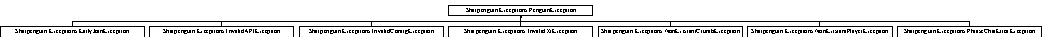
\includegraphics[height=0.501567cm]{classSharpenguin_1_1Exceptions_1_1PenguinException}
\end{center}
\end{figure}
\subsection*{Public Member Functions}
\begin{DoxyCompactItemize}
\item 
\hypertarget{classSharpenguin_1_1Exceptions_1_1PenguinException_a871080c38a4495954b949a98e8f1607a}{{\bfseries Penguin\-Exception} (string str\-Message)}\label{classSharpenguin_1_1Exceptions_1_1PenguinException_a871080c38a4495954b949a98e8f1607a}

\item 
\hypertarget{classSharpenguin_1_1Exceptions_1_1PenguinException_ae22f86a910bc8ee138a0d3f7b9f724cc}{{\bfseries Penguin\-Exception} (string str\-Message, \hyperlink{classSharpenguin_1_1Exceptions_1_1PenguinException}{Penguin\-Exception} obj\-Exception)}\label{classSharpenguin_1_1Exceptions_1_1PenguinException_ae22f86a910bc8ee138a0d3f7b9f724cc}

\end{DoxyCompactItemize}


\subsection{Detailed Description}
\hyperlink{classSharpenguin_1_1Penguin}{Penguin} base exception class. 

The documentation for this class was generated from the following file\-:\begin{DoxyCompactItemize}
\item 
Penguin\-Exceptions.\-cs\end{DoxyCompactItemize}

\hypertarget{classSharpenguin_1_1Data_1_1PenguinPacket}{\section{Sharpenguin.\-Data.\-Penguin\-Packet Class Reference}
\label{classSharpenguin_1_1Data_1_1PenguinPacket}\index{Sharpenguin.\-Data.\-Penguin\-Packet@{Sharpenguin.\-Data.\-Penguin\-Packet}}
}
\subsection*{Public Types}
\begin{DoxyCompactItemize}
\item 
enum \hyperlink{classSharpenguin_1_1Data_1_1PenguinPacket_ad526acc6fc64aa52d0a2f13dc9afb111}{Packet\-Type} \{ {\bfseries Xml}, 
{\bfseries Xt}, 
{\bfseries Unknown}
 \}
\end{DoxyCompactItemize}
\subsection*{Public Member Functions}
\begin{DoxyCompactItemize}
\item 
\hyperlink{classSharpenguin_1_1Data_1_1PenguinPacket_af167a2ed27d9cd6aeb506f6386b3ab99}{Penguin\-Packet} (string str\-Packet)
\end{DoxyCompactItemize}
\subsection*{Properties}
\begin{DoxyCompactItemize}
\item 
\hypertarget{classSharpenguin_1_1Data_1_1PenguinPacket_ab6770a1a2631dafcd81ec6fd4744ce26}{\hyperlink{classSharpenguin_1_1Data_1_1PenguinPacket_ad526acc6fc64aa52d0a2f13dc9afb111}{Packet\-Type} \hyperlink{classSharpenguin_1_1Data_1_1PenguinPacket_ab6770a1a2631dafcd81ec6fd4744ce26}{Type}\hspace{0.3cm}{\ttfamily  \mbox{[}get\mbox{]}}}\label{classSharpenguin_1_1Data_1_1PenguinPacket_ab6770a1a2631dafcd81ec6fd4744ce26}

\begin{DoxyCompactList}\small\item\em Gets the type of packet (\hyperlink{namespaceSharpenguin_1_1Xt}{Xt}, Xml, Unknown) \end{DoxyCompactList}\item 
\hypertarget{classSharpenguin_1_1Data_1_1PenguinPacket_a0303d5d80ae608579fc83fe5a6c2f719}{string \hyperlink{classSharpenguin_1_1Data_1_1PenguinPacket_a0303d5d80ae608579fc83fe5a6c2f719}{Data}\hspace{0.3cm}{\ttfamily  \mbox{[}get\mbox{]}}}\label{classSharpenguin_1_1Data_1_1PenguinPacket_a0303d5d80ae608579fc83fe5a6c2f719}

\begin{DoxyCompactList}\small\item\em Gets the string of data received in the packet. \end{DoxyCompactList}\item 
\hypertarget{classSharpenguin_1_1Data_1_1PenguinPacket_a93909a2441e03050635ffc5348179093}{\hyperlink{classSharpenguin_1_1Xt_1_1XtParser}{Xt.\-Xt\-Parser} \hyperlink{classSharpenguin_1_1Data_1_1PenguinPacket_a93909a2441e03050635ffc5348179093}{Xt}\hspace{0.3cm}{\ttfamily  \mbox{[}get\mbox{]}}}\label{classSharpenguin_1_1Data_1_1PenguinPacket_a93909a2441e03050635ffc5348179093}

\begin{DoxyCompactList}\small\item\em Gets the parsed \hyperlink{namespaceSharpenguin_1_1Xt}{Xt} string object (if the packet is \hyperlink{namespaceSharpenguin_1_1Xt}{Xt}). \end{DoxyCompactList}\item 
\hypertarget{classSharpenguin_1_1Data_1_1PenguinPacket_a7a8a1be17f28cd0ea097a24ed4e1bfb9}{System.\-Xml.\-Xml\-Element \hyperlink{classSharpenguin_1_1Data_1_1PenguinPacket_a7a8a1be17f28cd0ea097a24ed4e1bfb9}{Xml}\hspace{0.3cm}{\ttfamily  \mbox{[}get\mbox{]}}}\label{classSharpenguin_1_1Data_1_1PenguinPacket_a7a8a1be17f28cd0ea097a24ed4e1bfb9}

\begin{DoxyCompactList}\small\item\em Gets the parsed Xml string object (if the packet is Xml). \end{DoxyCompactList}\item 
\hypertarget{classSharpenguin_1_1Data_1_1PenguinPacket_aaaba175295e31224b549598e97dec87a}{int \hyperlink{classSharpenguin_1_1Data_1_1PenguinPacket_aaaba175295e31224b549598e97dec87a}{Length}\hspace{0.3cm}{\ttfamily  \mbox{[}get\mbox{]}}}\label{classSharpenguin_1_1Data_1_1PenguinPacket_aaaba175295e31224b549598e97dec87a}

\begin{DoxyCompactList}\small\item\em Gets the length of the packet. \end{DoxyCompactList}\end{DoxyCompactItemize}


\subsection{Detailed Description}
Stores and parses information about packets. 

\subsection{Member Enumeration Documentation}
\hypertarget{classSharpenguin_1_1Data_1_1PenguinPacket_ad526acc6fc64aa52d0a2f13dc9afb111}{\index{Sharpenguin\-::\-Data\-::\-Penguin\-Packet@{Sharpenguin\-::\-Data\-::\-Penguin\-Packet}!Packet\-Type@{Packet\-Type}}
\index{Packet\-Type@{Packet\-Type}!Sharpenguin::Data::PenguinPacket@{Sharpenguin\-::\-Data\-::\-Penguin\-Packet}}
\subsubsection[{Packet\-Type}]{\setlength{\rightskip}{0pt plus 5cm}enum {\bf Sharpenguin.\-Data.\-Penguin\-Packet.\-Packet\-Type}}}\label{classSharpenguin_1_1Data_1_1PenguinPacket_ad526acc6fc64aa52d0a2f13dc9afb111}
Enumeration of packet types. 

\subsection{Constructor \& Destructor Documentation}
\hypertarget{classSharpenguin_1_1Data_1_1PenguinPacket_af167a2ed27d9cd6aeb506f6386b3ab99}{\index{Sharpenguin\-::\-Data\-::\-Penguin\-Packet@{Sharpenguin\-::\-Data\-::\-Penguin\-Packet}!Penguin\-Packet@{Penguin\-Packet}}
\index{Penguin\-Packet@{Penguin\-Packet}!Sharpenguin::Data::PenguinPacket@{Sharpenguin\-::\-Data\-::\-Penguin\-Packet}}
\subsubsection[{Penguin\-Packet}]{\setlength{\rightskip}{0pt plus 5cm}Sharpenguin.\-Data.\-Penguin\-Packet.\-Penguin\-Packet (
\begin{DoxyParamCaption}
\item[{string}]{str\-Packet}
\end{DoxyParamCaption}
)\hspace{0.3cm}{\ttfamily [inline]}}}\label{classSharpenguin_1_1Data_1_1PenguinPacket_af167a2ed27d9cd6aeb506f6386b3ab99}
\hyperlink{classSharpenguin_1_1Data_1_1PenguinPacket}{Penguin\-Packet} constructor. Stores and parses the packet.


\begin{DoxyParams}{Parameters}
{\em str\-Packet} & Packet to parse and store. \\
\hline
\end{DoxyParams}


The documentation for this class was generated from the following file\-:\begin{DoxyCompactItemize}
\item 
Penguin\-Packet.\-cs\end{DoxyCompactItemize}

\hypertarget{classSharpenguin_1_1Data_1_1PenguinRoom}{\section{Sharpenguin.\-Data.\-Penguin\-Room Class Reference}
\label{classSharpenguin_1_1Data_1_1PenguinRoom}\index{Sharpenguin.\-Data.\-Penguin\-Room@{Sharpenguin.\-Data.\-Penguin\-Room}}
}
\subsection*{Public Member Functions}
\begin{DoxyCompactItemize}
\item 
void \hyperlink{classSharpenguin_1_1Data_1_1PenguinRoom_a6eb23989f397ce69a2365aff0ee42adb}{Change\-Room} (string room\-Name, int room\-Id, int ext\-Id)
\item 
void \hyperlink{classSharpenguin_1_1Data_1_1PenguinRoom_a1499f4cd3bd32d41e11c6a8cd0c70de4}{Add\-Self} (\hyperlink{classSharpenguin_1_1Data_1_1MyPlayer}{My\-Player} new\-Player)
\item 
void \hyperlink{classSharpenguin_1_1Data_1_1PenguinRoom_a25c1b2ce59c3cd19d90d3e4d76929788}{Add\-Player} (\hyperlink{classSharpenguin_1_1Data_1_1Player}{Player} new\-Player)
\item 
\hyperlink{classSharpenguin_1_1Data_1_1Player}{Player} \hyperlink{classSharpenguin_1_1Data_1_1PenguinRoom_a2b9490bdf704b051a9b1edcdaeb420ab}{Get\-Player} (int int\-Id)
\item 
bool \hyperlink{classSharpenguin_1_1Data_1_1PenguinRoom_aac8f948d0d296520efc706c6a22a2b11}{Try\-Get\-Player} (int int\-Id, out \hyperlink{classSharpenguin_1_1Data_1_1Player}{Player} got\-Player)
\item 
bool \hyperlink{classSharpenguin_1_1Data_1_1PenguinRoom_a11e805d83a9b2769d5dfbbe6931ef4e8}{Try\-Get\-Player\-By\-Name} (string penguin\-Name, out \hyperlink{classSharpenguin_1_1Data_1_1Player}{Player} got\-Player)
\item 
bool \hyperlink{classSharpenguin_1_1Data_1_1PenguinRoom_a2843fba06f2bd503a09a89e0e6ba87fa}{Remove\-Player} (int int\-Id)
\item 
bool \hyperlink{classSharpenguin_1_1Data_1_1PenguinRoom_a5a613e61b542886c45f3b9eb7cd17c53}{Remove\-Player\-By\-Name} (string penguin\-Name)
\item 
bool \hyperlink{classSharpenguin_1_1Data_1_1PenguinRoom_ac0851db56a7e51dfa7a542483157eb8e}{Has\-Player} (int int\-Id)
\end{DoxyCompactItemize}
\subsection*{Properties}
\begin{DoxyCompactItemize}
\item 
\hypertarget{classSharpenguin_1_1Data_1_1PenguinRoom_ad18150861add37e0b379e1d1ad1dce08}{string \hyperlink{classSharpenguin_1_1Data_1_1PenguinRoom_ad18150861add37e0b379e1d1ad1dce08}{Name}\hspace{0.3cm}{\ttfamily  \mbox{[}get\mbox{]}}}\label{classSharpenguin_1_1Data_1_1PenguinRoom_ad18150861add37e0b379e1d1ad1dce08}

\begin{DoxyCompactList}\small\item\em Gets the name of the room. \end{DoxyCompactList}\item 
\hypertarget{classSharpenguin_1_1Data_1_1PenguinRoom_a223a3cbc592600dee66427838e926956}{int \hyperlink{classSharpenguin_1_1Data_1_1PenguinRoom_a223a3cbc592600dee66427838e926956}{Int\-I\-D}\hspace{0.3cm}{\ttfamily  \mbox{[}get\mbox{]}}}\label{classSharpenguin_1_1Data_1_1PenguinRoom_a223a3cbc592600dee66427838e926956}

\begin{DoxyCompactList}\small\item\em Gets the internal I\-D of the room. \end{DoxyCompactList}\item 
\hypertarget{classSharpenguin_1_1Data_1_1PenguinRoom_a4ce2da1fa1e871bd07dd6fe2fa82d6c1}{int \hyperlink{classSharpenguin_1_1Data_1_1PenguinRoom_a4ce2da1fa1e871bd07dd6fe2fa82d6c1}{Ext\-I\-D}\hspace{0.3cm}{\ttfamily  \mbox{[}get\mbox{]}}}\label{classSharpenguin_1_1Data_1_1PenguinRoom_a4ce2da1fa1e871bd07dd6fe2fa82d6c1}

\begin{DoxyCompactList}\small\item\em Gets the external I\-D of the room. \end{DoxyCompactList}\item 
\hypertarget{classSharpenguin_1_1Data_1_1PenguinRoom_ac657d32b534bb38fc39ca0a1041e86c1}{\hyperlink{classSharpenguin_1_1Data_1_1Player}{Player}\mbox{[}$\,$\mbox{]} \hyperlink{classSharpenguin_1_1Data_1_1PenguinRoom_ac657d32b534bb38fc39ca0a1041e86c1}{Players}\hspace{0.3cm}{\ttfamily  \mbox{[}get\mbox{]}}}\label{classSharpenguin_1_1Data_1_1PenguinRoom_ac657d32b534bb38fc39ca0a1041e86c1}

\begin{DoxyCompactList}\small\item\em Gets the dictionary of players. \end{DoxyCompactList}\item 
\hypertarget{classSharpenguin_1_1Data_1_1PenguinRoom_af65781b1023d9b172ccecda1bcd4baa3}{\hyperlink{classSharpenguin_1_1Data_1_1MyPlayer}{My\-Player} \hyperlink{classSharpenguin_1_1Data_1_1PenguinRoom_af65781b1023d9b172ccecda1bcd4baa3}{Self}\hspace{0.3cm}{\ttfamily  \mbox{[}get\mbox{]}}}\label{classSharpenguin_1_1Data_1_1PenguinRoom_af65781b1023d9b172ccecda1bcd4baa3}

\begin{DoxyCompactList}\small\item\em Gets your own player. \end{DoxyCompactList}\end{DoxyCompactItemize}


\subsection{Detailed Description}
Stores information about a room, including players, name and ids. 

\subsection{Member Function Documentation}
\hypertarget{classSharpenguin_1_1Data_1_1PenguinRoom_a25c1b2ce59c3cd19d90d3e4d76929788}{\index{Sharpenguin\-::\-Data\-::\-Penguin\-Room@{Sharpenguin\-::\-Data\-::\-Penguin\-Room}!Add\-Player@{Add\-Player}}
\index{Add\-Player@{Add\-Player}!Sharpenguin::Data::PenguinRoom@{Sharpenguin\-::\-Data\-::\-Penguin\-Room}}
\subsubsection[{Add\-Player}]{\setlength{\rightskip}{0pt plus 5cm}void Sharpenguin.\-Data.\-Penguin\-Room.\-Add\-Player (
\begin{DoxyParamCaption}
\item[{{\bf Player}}]{new\-Player}
\end{DoxyParamCaption}
)\hspace{0.3cm}{\ttfamily [inline]}}}\label{classSharpenguin_1_1Data_1_1PenguinRoom_a25c1b2ce59c3cd19d90d3e4d76929788}
Adds a player to the room.


\begin{DoxyParams}{Parameters}
{\em new\-Player} & The player to add. \\
\hline
\end{DoxyParams}
\hypertarget{classSharpenguin_1_1Data_1_1PenguinRoom_a1499f4cd3bd32d41e11c6a8cd0c70de4}{\index{Sharpenguin\-::\-Data\-::\-Penguin\-Room@{Sharpenguin\-::\-Data\-::\-Penguin\-Room}!Add\-Self@{Add\-Self}}
\index{Add\-Self@{Add\-Self}!Sharpenguin::Data::PenguinRoom@{Sharpenguin\-::\-Data\-::\-Penguin\-Room}}
\subsubsection[{Add\-Self}]{\setlength{\rightskip}{0pt plus 5cm}void Sharpenguin.\-Data.\-Penguin\-Room.\-Add\-Self (
\begin{DoxyParamCaption}
\item[{{\bf My\-Player}}]{new\-Player}
\end{DoxyParamCaption}
)\hspace{0.3cm}{\ttfamily [inline]}}}\label{classSharpenguin_1_1Data_1_1PenguinRoom_a1499f4cd3bd32d41e11c6a8cd0c70de4}
Adds your own player to the room.


\begin{DoxyParams}{Parameters}
{\em new\-Player} & Your player object. \\
\hline
\end{DoxyParams}
\hypertarget{classSharpenguin_1_1Data_1_1PenguinRoom_a6eb23989f397ce69a2365aff0ee42adb}{\index{Sharpenguin\-::\-Data\-::\-Penguin\-Room@{Sharpenguin\-::\-Data\-::\-Penguin\-Room}!Change\-Room@{Change\-Room}}
\index{Change\-Room@{Change\-Room}!Sharpenguin::Data::PenguinRoom@{Sharpenguin\-::\-Data\-::\-Penguin\-Room}}
\subsubsection[{Change\-Room}]{\setlength{\rightskip}{0pt plus 5cm}void Sharpenguin.\-Data.\-Penguin\-Room.\-Change\-Room (
\begin{DoxyParamCaption}
\item[{string}]{room\-Name, }
\item[{int}]{room\-Id, }
\item[{int}]{ext\-Id}
\end{DoxyParamCaption}
)\hspace{0.3cm}{\ttfamily [inline]}}}\label{classSharpenguin_1_1Data_1_1PenguinRoom_a6eb23989f397ce69a2365aff0ee42adb}
Changes the room.


\begin{DoxyParams}{Parameters}
{\em room\-Name} & The name of the room.\\
\hline
{\em room\-Id} & The internal id of the room.\\
\hline
{\em ext\-Id} & The external id of the room. \\
\hline
\end{DoxyParams}
\hypertarget{classSharpenguin_1_1Data_1_1PenguinRoom_a2b9490bdf704b051a9b1edcdaeb420ab}{\index{Sharpenguin\-::\-Data\-::\-Penguin\-Room@{Sharpenguin\-::\-Data\-::\-Penguin\-Room}!Get\-Player@{Get\-Player}}
\index{Get\-Player@{Get\-Player}!Sharpenguin::Data::PenguinRoom@{Sharpenguin\-::\-Data\-::\-Penguin\-Room}}
\subsubsection[{Get\-Player}]{\setlength{\rightskip}{0pt plus 5cm}{\bf Player} Sharpenguin.\-Data.\-Penguin\-Room.\-Get\-Player (
\begin{DoxyParamCaption}
\item[{int}]{int\-Id}
\end{DoxyParamCaption}
)\hspace{0.3cm}{\ttfamily [inline]}}}\label{classSharpenguin_1_1Data_1_1PenguinRoom_a2b9490bdf704b051a9b1edcdaeb420ab}
Gets a player from the room via their I\-D.


\begin{DoxyParams}{Parameters}
{\em int\-Id} & The player's id. \\
\hline
\end{DoxyParams}
\hypertarget{classSharpenguin_1_1Data_1_1PenguinRoom_ac0851db56a7e51dfa7a542483157eb8e}{\index{Sharpenguin\-::\-Data\-::\-Penguin\-Room@{Sharpenguin\-::\-Data\-::\-Penguin\-Room}!Has\-Player@{Has\-Player}}
\index{Has\-Player@{Has\-Player}!Sharpenguin::Data::PenguinRoom@{Sharpenguin\-::\-Data\-::\-Penguin\-Room}}
\subsubsection[{Has\-Player}]{\setlength{\rightskip}{0pt plus 5cm}bool Sharpenguin.\-Data.\-Penguin\-Room.\-Has\-Player (
\begin{DoxyParamCaption}
\item[{int}]{int\-Id}
\end{DoxyParamCaption}
)\hspace{0.3cm}{\ttfamily [inline]}}}\label{classSharpenguin_1_1Data_1_1PenguinRoom_ac0851db56a7e51dfa7a542483157eb8e}
Determines whether the player is in the room or not.


\begin{DoxyParams}{Parameters}
{\em int\-Id} & The id of the player to find.\\
\hline
\end{DoxyParams}
\begin{DoxyReturn}{Returns}
T\-R\-U\-E if the player is in the room, F\-A\-L\-S\-E if they are not. 
\end{DoxyReturn}
\hypertarget{classSharpenguin_1_1Data_1_1PenguinRoom_a2843fba06f2bd503a09a89e0e6ba87fa}{\index{Sharpenguin\-::\-Data\-::\-Penguin\-Room@{Sharpenguin\-::\-Data\-::\-Penguin\-Room}!Remove\-Player@{Remove\-Player}}
\index{Remove\-Player@{Remove\-Player}!Sharpenguin::Data::PenguinRoom@{Sharpenguin\-::\-Data\-::\-Penguin\-Room}}
\subsubsection[{Remove\-Player}]{\setlength{\rightskip}{0pt plus 5cm}bool Sharpenguin.\-Data.\-Penguin\-Room.\-Remove\-Player (
\begin{DoxyParamCaption}
\item[{int}]{int\-Id}
\end{DoxyParamCaption}
)\hspace{0.3cm}{\ttfamily [inline]}}}\label{classSharpenguin_1_1Data_1_1PenguinRoom_a2843fba06f2bd503a09a89e0e6ba87fa}
Removes a player from the room via their I\-D.


\begin{DoxyParams}{Parameters}
{\em int\-Id} & The id of the player to remove.\\
\hline
\end{DoxyParams}
\begin{DoxyReturn}{Returns}
T\-R\-U\-E on success, F\-A\-L\-S\-E on failure. 
\end{DoxyReturn}
\hypertarget{classSharpenguin_1_1Data_1_1PenguinRoom_a5a613e61b542886c45f3b9eb7cd17c53}{\index{Sharpenguin\-::\-Data\-::\-Penguin\-Room@{Sharpenguin\-::\-Data\-::\-Penguin\-Room}!Remove\-Player\-By\-Name@{Remove\-Player\-By\-Name}}
\index{Remove\-Player\-By\-Name@{Remove\-Player\-By\-Name}!Sharpenguin::Data::PenguinRoom@{Sharpenguin\-::\-Data\-::\-Penguin\-Room}}
\subsubsection[{Remove\-Player\-By\-Name}]{\setlength{\rightskip}{0pt plus 5cm}bool Sharpenguin.\-Data.\-Penguin\-Room.\-Remove\-Player\-By\-Name (
\begin{DoxyParamCaption}
\item[{string}]{penguin\-Name}
\end{DoxyParamCaption}
)\hspace{0.3cm}{\ttfamily [inline]}}}\label{classSharpenguin_1_1Data_1_1PenguinRoom_a5a613e61b542886c45f3b9eb7cd17c53}
Removes a player from the room via their name.


\begin{DoxyParams}{Parameters}
{\em penguin\-Name} & The the name of the player to remove.\\
\hline
\end{DoxyParams}
\begin{DoxyReturn}{Returns}
T\-R\-U\-E on success, F\-A\-L\-S\-E on failure. 
\end{DoxyReturn}
\hypertarget{classSharpenguin_1_1Data_1_1PenguinRoom_aac8f948d0d296520efc706c6a22a2b11}{\index{Sharpenguin\-::\-Data\-::\-Penguin\-Room@{Sharpenguin\-::\-Data\-::\-Penguin\-Room}!Try\-Get\-Player@{Try\-Get\-Player}}
\index{Try\-Get\-Player@{Try\-Get\-Player}!Sharpenguin::Data::PenguinRoom@{Sharpenguin\-::\-Data\-::\-Penguin\-Room}}
\subsubsection[{Try\-Get\-Player}]{\setlength{\rightskip}{0pt plus 5cm}bool Sharpenguin.\-Data.\-Penguin\-Room.\-Try\-Get\-Player (
\begin{DoxyParamCaption}
\item[{int}]{int\-Id, }
\item[{out {\bf Player}}]{got\-Player}
\end{DoxyParamCaption}
)\hspace{0.3cm}{\ttfamily [inline]}}}\label{classSharpenguin_1_1Data_1_1PenguinRoom_aac8f948d0d296520efc706c6a22a2b11}
Tries to get a player from the room via their I\-D.


\begin{DoxyParams}{Parameters}
{\em int\-Id} & The player's id. \\
\hline
{\em got\-Player} & The found player (if it exists).\\
\hline
\end{DoxyParams}
\begin{DoxyReturn}{Returns}
T\-R\-U\-E if the player is found, F\-A\-L\-S\-E if it is not. 
\end{DoxyReturn}
\hypertarget{classSharpenguin_1_1Data_1_1PenguinRoom_a11e805d83a9b2769d5dfbbe6931ef4e8}{\index{Sharpenguin\-::\-Data\-::\-Penguin\-Room@{Sharpenguin\-::\-Data\-::\-Penguin\-Room}!Try\-Get\-Player\-By\-Name@{Try\-Get\-Player\-By\-Name}}
\index{Try\-Get\-Player\-By\-Name@{Try\-Get\-Player\-By\-Name}!Sharpenguin::Data::PenguinRoom@{Sharpenguin\-::\-Data\-::\-Penguin\-Room}}
\subsubsection[{Try\-Get\-Player\-By\-Name}]{\setlength{\rightskip}{0pt plus 5cm}bool Sharpenguin.\-Data.\-Penguin\-Room.\-Try\-Get\-Player\-By\-Name (
\begin{DoxyParamCaption}
\item[{string}]{penguin\-Name, }
\item[{out {\bf Player}}]{got\-Player}
\end{DoxyParamCaption}
)\hspace{0.3cm}{\ttfamily [inline]}}}\label{classSharpenguin_1_1Data_1_1PenguinRoom_a11e805d83a9b2769d5dfbbe6931ef4e8}
Tries to get a player from the room via their name.


\begin{DoxyParams}{Parameters}
{\em penuin\-Name} & The username of the penguin.\\
\hline
{\em got\-Player} & The found player (if it exists).\\
\hline
\end{DoxyParams}
\begin{DoxyReturn}{Returns}
T\-R\-U\-E if the player is found, F\-A\-L\-S\-E if it is not. 
\end{DoxyReturn}


The documentation for this class was generated from the following file\-:\begin{DoxyCompactItemize}
\item 
Penguin\-Room.\-cs\end{DoxyCompactItemize}

\hypertarget{classSharpenguin_1_1Net_1_1PenguinSocket}{\section{Sharpenguin.\-Net.\-Penguin\-Socket Class Reference}
\label{classSharpenguin_1_1Net_1_1PenguinSocket}\index{Sharpenguin.\-Net.\-Penguin\-Socket@{Sharpenguin.\-Net.\-Penguin\-Socket}}
}
\subsection*{Public Member Functions}
\begin{DoxyCompactItemize}
\item 
void \hyperlink{classSharpenguin_1_1Net_1_1PenguinSocket_a6508a955d89a5aa6a51f8bfac2f52b3e}{Begin\-Connect} (string str\-Host, int int\-Port, Penguin\-Connect\-Callback connect\-Callback)
\item 
void \hyperlink{classSharpenguin_1_1Net_1_1PenguinSocket_ac6fc724da56b753de71deb6aea0d473e}{Connection\-Callback} (System.\-I\-Async\-Result async\-Result)
\item 
void \hyperlink{classSharpenguin_1_1Net_1_1PenguinSocket_ac60926b98466d10e0db01bd48c4b4ad8}{Disconnect} ()
\item 
void \hyperlink{classSharpenguin_1_1Net_1_1PenguinSocket_af55abe0b108fa3b4e94e20a639812b32}{Begin\-Receive} (Penguin\-Receive\-Callback receive\-Callback, Penguin\-Disconnect\-Callback disconnect\-Callback)
\item 
void \hyperlink{classSharpenguin_1_1Net_1_1PenguinSocket_a1a22198956191adbdfcd2649d141f8f6}{Begin\-Write} (string str\-Data)
\item 
void \hyperlink{classSharpenguin_1_1Net_1_1PenguinSocket_a08bb8907688a36801115b1797aca2542}{Send\-Callback} (System.\-I\-Async\-Result async\-Result)
\end{DoxyCompactItemize}
\subsection*{Properties}
\begin{DoxyCompactItemize}
\item 
\hypertarget{classSharpenguin_1_1Net_1_1PenguinSocket_aebcbb81e484814de900b1254e0798717}{bool \hyperlink{classSharpenguin_1_1Net_1_1PenguinSocket_aebcbb81e484814de900b1254e0798717}{Connected}\hspace{0.3cm}{\ttfamily  \mbox{[}get\mbox{]}}}\label{classSharpenguin_1_1Net_1_1PenguinSocket_aebcbb81e484814de900b1254e0798717}

\begin{DoxyCompactList}\small\item\em Gets whether or not the socket is connected. \end{DoxyCompactList}\end{DoxyCompactItemize}


\subsection{Detailed Description}
Socket wrapper for penguin. Incorporates asynchronous reading until \textbackslash{}0. 

\subsection{Member Function Documentation}
\hypertarget{classSharpenguin_1_1Net_1_1PenguinSocket_a6508a955d89a5aa6a51f8bfac2f52b3e}{\index{Sharpenguin\-::\-Net\-::\-Penguin\-Socket@{Sharpenguin\-::\-Net\-::\-Penguin\-Socket}!Begin\-Connect@{Begin\-Connect}}
\index{Begin\-Connect@{Begin\-Connect}!Sharpenguin::Net::PenguinSocket@{Sharpenguin\-::\-Net\-::\-Penguin\-Socket}}
\subsubsection[{Begin\-Connect}]{\setlength{\rightskip}{0pt plus 5cm}void Sharpenguin.\-Net.\-Penguin\-Socket.\-Begin\-Connect (
\begin{DoxyParamCaption}
\item[{string}]{str\-Host, }
\item[{int}]{int\-Port, }
\item[{Penguin\-Connect\-Callback}]{connect\-Callback}
\end{DoxyParamCaption}
)\hspace{0.3cm}{\ttfamily [inline]}}}\label{classSharpenguin_1_1Net_1_1PenguinSocket_a6508a955d89a5aa6a51f8bfac2f52b3e}
Creates a new socket and connects to the specified host and port.


\begin{DoxyParams}{Parameters}
{\em str\-Host} & Host to connect to. \\
\hline
{\em int\-Port} & Port to connect to. \\
\hline
\end{DoxyParams}
\hypertarget{classSharpenguin_1_1Net_1_1PenguinSocket_af55abe0b108fa3b4e94e20a639812b32}{\index{Sharpenguin\-::\-Net\-::\-Penguin\-Socket@{Sharpenguin\-::\-Net\-::\-Penguin\-Socket}!Begin\-Receive@{Begin\-Receive}}
\index{Begin\-Receive@{Begin\-Receive}!Sharpenguin::Net::PenguinSocket@{Sharpenguin\-::\-Net\-::\-Penguin\-Socket}}
\subsubsection[{Begin\-Receive}]{\setlength{\rightskip}{0pt plus 5cm}void Sharpenguin.\-Net.\-Penguin\-Socket.\-Begin\-Receive (
\begin{DoxyParamCaption}
\item[{Penguin\-Receive\-Callback}]{receive\-Callback, }
\item[{Penguin\-Disconnect\-Callback}]{disconnect\-Callback}
\end{DoxyParamCaption}
)\hspace{0.3cm}{\ttfamily [inline]}}}\label{classSharpenguin_1_1Net_1_1PenguinSocket_af55abe0b108fa3b4e94e20a639812b32}
Begins asynchronous receiving.


\begin{DoxyParams}{Parameters}
{\em receive\-Del} & The callback to trigger when a packet is received. \\
\hline
{\em disconnect\-Del} & The callback to trigger when an error occurs. \\
\hline
\end{DoxyParams}
\hypertarget{classSharpenguin_1_1Net_1_1PenguinSocket_a1a22198956191adbdfcd2649d141f8f6}{\index{Sharpenguin\-::\-Net\-::\-Penguin\-Socket@{Sharpenguin\-::\-Net\-::\-Penguin\-Socket}!Begin\-Write@{Begin\-Write}}
\index{Begin\-Write@{Begin\-Write}!Sharpenguin::Net::PenguinSocket@{Sharpenguin\-::\-Net\-::\-Penguin\-Socket}}
\subsubsection[{Begin\-Write}]{\setlength{\rightskip}{0pt plus 5cm}void Sharpenguin.\-Net.\-Penguin\-Socket.\-Begin\-Write (
\begin{DoxyParamCaption}
\item[{string}]{str\-Data}
\end{DoxyParamCaption}
)\hspace{0.3cm}{\ttfamily [inline]}}}\label{classSharpenguin_1_1Net_1_1PenguinSocket_a1a22198956191adbdfcd2649d141f8f6}
Begins asynchronous writing.


\begin{DoxyParams}{Parameters}
{\em str\-Data} & The data to send. \\
\hline
\end{DoxyParams}
\hypertarget{classSharpenguin_1_1Net_1_1PenguinSocket_ac6fc724da56b753de71deb6aea0d473e}{\index{Sharpenguin\-::\-Net\-::\-Penguin\-Socket@{Sharpenguin\-::\-Net\-::\-Penguin\-Socket}!Connection\-Callback@{Connection\-Callback}}
\index{Connection\-Callback@{Connection\-Callback}!Sharpenguin::Net::PenguinSocket@{Sharpenguin\-::\-Net\-::\-Penguin\-Socket}}
\subsubsection[{Connection\-Callback}]{\setlength{\rightskip}{0pt plus 5cm}void Sharpenguin.\-Net.\-Penguin\-Socket.\-Connection\-Callback (
\begin{DoxyParamCaption}
\item[{System.\-I\-Async\-Result}]{async\-Result}
\end{DoxyParamCaption}
)\hspace{0.3cm}{\ttfamily [inline]}}}\label{classSharpenguin_1_1Net_1_1PenguinSocket_ac6fc724da56b753de71deb6aea0d473e}
Handles connection success or failure.


\begin{DoxyParams}{Parameters}
{\em async\-Result} & The I\-Async\-Result of the connection attempt. \\
\hline
\end{DoxyParams}
\hypertarget{classSharpenguin_1_1Net_1_1PenguinSocket_ac60926b98466d10e0db01bd48c4b4ad8}{\index{Sharpenguin\-::\-Net\-::\-Penguin\-Socket@{Sharpenguin\-::\-Net\-::\-Penguin\-Socket}!Disconnect@{Disconnect}}
\index{Disconnect@{Disconnect}!Sharpenguin::Net::PenguinSocket@{Sharpenguin\-::\-Net\-::\-Penguin\-Socket}}
\subsubsection[{Disconnect}]{\setlength{\rightskip}{0pt plus 5cm}void Sharpenguin.\-Net.\-Penguin\-Socket.\-Disconnect (
\begin{DoxyParamCaption}
{}
\end{DoxyParamCaption}
)\hspace{0.3cm}{\ttfamily [inline]}}}\label{classSharpenguin_1_1Net_1_1PenguinSocket_ac60926b98466d10e0db01bd48c4b4ad8}
Closes the socket connection. \hypertarget{classSharpenguin_1_1Net_1_1PenguinSocket_a08bb8907688a36801115b1797aca2542}{\index{Sharpenguin\-::\-Net\-::\-Penguin\-Socket@{Sharpenguin\-::\-Net\-::\-Penguin\-Socket}!Send\-Callback@{Send\-Callback}}
\index{Send\-Callback@{Send\-Callback}!Sharpenguin::Net::PenguinSocket@{Sharpenguin\-::\-Net\-::\-Penguin\-Socket}}
\subsubsection[{Send\-Callback}]{\setlength{\rightskip}{0pt plus 5cm}void Sharpenguin.\-Net.\-Penguin\-Socket.\-Send\-Callback (
\begin{DoxyParamCaption}
\item[{System.\-I\-Async\-Result}]{async\-Result}
\end{DoxyParamCaption}
)\hspace{0.3cm}{\ttfamily [inline]}}}\label{classSharpenguin_1_1Net_1_1PenguinSocket_a08bb8907688a36801115b1797aca2542}
Ends asynchronous sending.


\begin{DoxyParams}{Parameters}
{\em async\-Result} & The I\-Async\-Result returned from the asynchronous sending. \\
\hline
\end{DoxyParams}


The documentation for this class was generated from the following file\-:\begin{DoxyCompactItemize}
\item 
Penguin\-Socket.\-cs\end{DoxyCompactItemize}

\hypertarget{classSharpenguin_1_1Exceptions_1_1PhraseChatErrorException}{\section{\-Sharpenguin.\-Exceptions.\-Phrase\-Chat\-Error\-Exception \-Class \-Reference}
\label{classSharpenguin_1_1Exceptions_1_1PhraseChatErrorException}\index{\-Sharpenguin.\-Exceptions.\-Phrase\-Chat\-Error\-Exception@{\-Sharpenguin.\-Exceptions.\-Phrase\-Chat\-Error\-Exception}}
}
\-Inheritance diagram for \-Sharpenguin.\-Exceptions.\-Phrase\-Chat\-Error\-Exception\-:\begin{figure}[H]
\begin{center}
\leavevmode
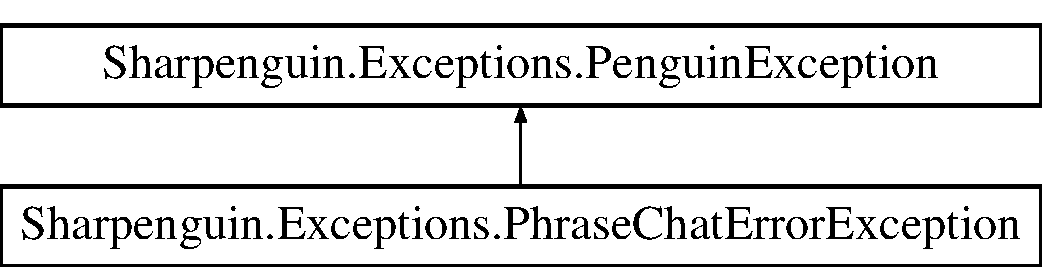
\includegraphics[height=2.000000cm]{classSharpenguin_1_1Exceptions_1_1PhraseChatErrorException}
\end{center}
\end{figure}
\subsection*{\-Public \-Member \-Functions}
\begin{DoxyCompactItemize}
\item 
\hypertarget{classSharpenguin_1_1Exceptions_1_1PhraseChatErrorException_a358dfb96b642ea8490c016132052bf0e}{{\bfseries \-Phrase\-Chat\-Error\-Exception} (string str\-Message)}\label{classSharpenguin_1_1Exceptions_1_1PhraseChatErrorException_a358dfb96b642ea8490c016132052bf0e}

\item 
\hypertarget{classSharpenguin_1_1Exceptions_1_1PhraseChatErrorException_aef532df77cc555e2b985336ea4fea714}{{\bfseries \-Phrase\-Chat\-Error\-Exception} (string str\-Message, \hyperlink{classSharpenguin_1_1Exceptions_1_1PhraseChatErrorException}{\-Phrase\-Chat\-Error\-Exception} obj\-Exception)}\label{classSharpenguin_1_1Exceptions_1_1PhraseChatErrorException_aef532df77cc555e2b985336ea4fea714}

\end{DoxyCompactItemize}


\subsection{\-Detailed \-Description}
\-Exception for when there was an error in parsing the phrase chat message. 

\-The documentation for this class was generated from the following file\-:\begin{DoxyCompactItemize}
\item 
\-Penguin\-Exceptions.\-cs\end{DoxyCompactItemize}

\hypertarget{classSharpenguin_1_1Data_1_1Player}{\section{\-Sharpenguin.\-Data.\-Player \-Class \-Reference}
\label{classSharpenguin_1_1Data_1_1Player}\index{\-Sharpenguin.\-Data.\-Player@{\-Sharpenguin.\-Data.\-Player}}
}
\-Inheritance diagram for \-Sharpenguin.\-Data.\-Player\-:\begin{figure}[H]
\begin{center}
\leavevmode
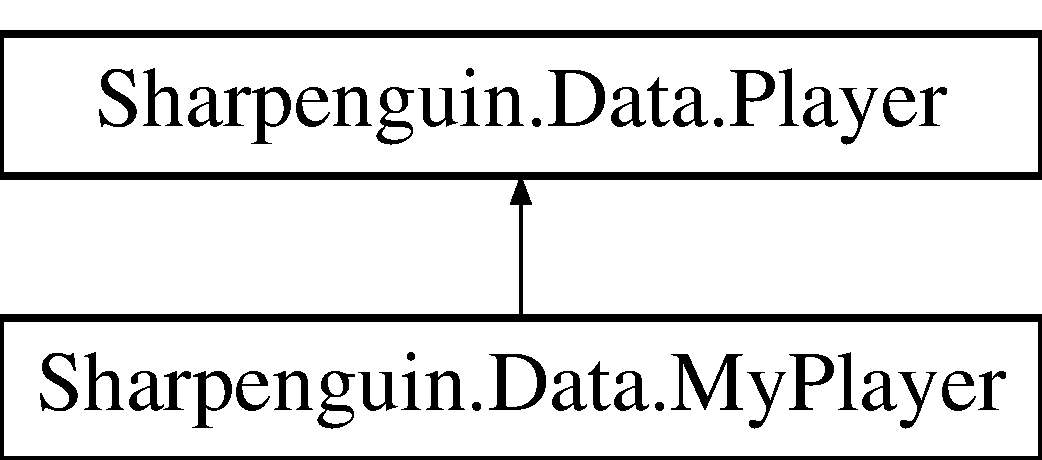
\includegraphics[height=2.000000cm]{classSharpenguin_1_1Data_1_1Player}
\end{center}
\end{figure}
\subsection*{\-Public \-Member \-Functions}
\begin{DoxyCompactItemize}
\item 
void \hyperlink{classSharpenguin_1_1Data_1_1Player_a22a732a7064e1ce773d624602527c880}{\-Load\-Data} (string str\-Data)
\end{DoxyCompactItemize}
\subsection*{\-Properties}
\begin{DoxyCompactItemize}
\item 
\hypertarget{classSharpenguin_1_1Data_1_1Player_a2607a3c888d2a6e67fdf6f3f5a5e75ec}{int {\bfseries \-Id}\hspace{0.3cm}{\ttfamily  \mbox{[}get\mbox{]}}}\label{classSharpenguin_1_1Data_1_1Player_a2607a3c888d2a6e67fdf6f3f5a5e75ec}

\item 
\hypertarget{classSharpenguin_1_1Data_1_1Player_a7b2814bdcbf34bb2c51f77a43f39cecc}{int {\bfseries \-Member\-Days}\hspace{0.3cm}{\ttfamily  \mbox{[}get\mbox{]}}}\label{classSharpenguin_1_1Data_1_1Player_a7b2814bdcbf34bb2c51f77a43f39cecc}

\item 
\hypertarget{classSharpenguin_1_1Data_1_1Player_a35b25abceee8791586c924fb5c26829b}{int {\bfseries \-Time\-Zone\-Offset}\hspace{0.3cm}{\ttfamily  \mbox{[}get\mbox{]}}}\label{classSharpenguin_1_1Data_1_1Player_a35b25abceee8791586c924fb5c26829b}

\item 
\hypertarget{classSharpenguin_1_1Data_1_1Player_affeb3814ed1eb1e1649fc7001ef0a001}{string {\bfseries \-Username}\hspace{0.3cm}{\ttfamily  \mbox{[}get\mbox{]}}}\label{classSharpenguin_1_1Data_1_1Player_affeb3814ed1eb1e1649fc7001ef0a001}

\item 
\hypertarget{classSharpenguin_1_1Data_1_1Player_a8f5b48dcbddaafad975c0b3f50bda2ba}{bool {\bfseries \-Is\-Member}\hspace{0.3cm}{\ttfamily  \mbox{[}get\mbox{]}}}\label{classSharpenguin_1_1Data_1_1Player_a8f5b48dcbddaafad975c0b3f50bda2ba}

\item 
\hypertarget{classSharpenguin_1_1Data_1_1Player_afa90c904ed3d3619adf416cebba87e8d}{\hyperlink{classSharpenguin_1_1Data_1_1PlayerItem}{\-Player\-Item} {\bfseries \-Item}\hspace{0.3cm}{\ttfamily  \mbox{[}get\mbox{]}}}\label{classSharpenguin_1_1Data_1_1Player_afa90c904ed3d3619adf416cebba87e8d}

\item 
\hypertarget{classSharpenguin_1_1Data_1_1Player_a62696c934b11a3b448ee9959e76e029a}{\hyperlink{classSharpenguin_1_1Data_1_1PlayerPosition}{\-Player\-Position} {\bfseries \-Position}\hspace{0.3cm}{\ttfamily  \mbox{[}get\mbox{]}}}\label{classSharpenguin_1_1Data_1_1Player_a62696c934b11a3b448ee9959e76e029a}

\end{DoxyCompactItemize}


\subsection{\-Detailed \-Description}
\-The player class. \-Information about players in the room are stored here. 

\subsection{\-Member \-Function \-Documentation}
\hypertarget{classSharpenguin_1_1Data_1_1Player_a22a732a7064e1ce773d624602527c880}{\index{\-Sharpenguin\-::\-Data\-::\-Player@{\-Sharpenguin\-::\-Data\-::\-Player}!\-Load\-Data@{\-Load\-Data}}
\index{\-Load\-Data@{\-Load\-Data}!Sharpenguin::Data::Player@{\-Sharpenguin\-::\-Data\-::\-Player}}
\subsubsection[{\-Load\-Data}]{\setlength{\rightskip}{0pt plus 5cm}void {\bf \-Sharpenguin.\-Data.\-Player.\-Load\-Data} (
\begin{DoxyParamCaption}
\item[{string}]{str\-Data}
\end{DoxyParamCaption}
)\hspace{0.3cm}{\ttfamily  \mbox{[}inline\mbox{]}}}}\label{classSharpenguin_1_1Data_1_1Player_a22a732a7064e1ce773d624602527c880}
\-Constructor for the player class, loads the player data from the player string. 

\-The documentation for this class was generated from the following file\-:\begin{DoxyCompactItemize}
\item 
\-Player.\-cs\end{DoxyCompactItemize}

\hypertarget{classSharpenguin_1_1Data_1_1PlayerItem}{\section{\-Sharpenguin.\-Data.\-Player\-Item \-Class \-Reference}
\label{classSharpenguin_1_1Data_1_1PlayerItem}\index{\-Sharpenguin.\-Data.\-Player\-Item@{\-Sharpenguin.\-Data.\-Player\-Item}}
}
\subsection*{\-Public \-Member \-Functions}
\begin{DoxyCompactItemize}
\item 
\hypertarget{classSharpenguin_1_1Data_1_1PlayerItem_a0ba43aab58727760a20d0197519a2bd5}{void {\bfseries \-Set\-Colour} (int int\-Id)}\label{classSharpenguin_1_1Data_1_1PlayerItem_a0ba43aab58727760a20d0197519a2bd5}

\item 
\hypertarget{classSharpenguin_1_1Data_1_1PlayerItem_a7e92eb001d9fda4ac63a28d72e1dcb10}{void {\bfseries \-Set\-Head} (int int\-Id)}\label{classSharpenguin_1_1Data_1_1PlayerItem_a7e92eb001d9fda4ac63a28d72e1dcb10}

\item 
\hypertarget{classSharpenguin_1_1Data_1_1PlayerItem_acf3bf50435cba4d176a907acda3430a0}{void {\bfseries \-Set\-Face} (int int\-Id)}\label{classSharpenguin_1_1Data_1_1PlayerItem_acf3bf50435cba4d176a907acda3430a0}

\item 
\hypertarget{classSharpenguin_1_1Data_1_1PlayerItem_aa85fa149653805e76d0b08b1152e0628}{void {\bfseries \-Set\-Neck} (int int\-Id)}\label{classSharpenguin_1_1Data_1_1PlayerItem_aa85fa149653805e76d0b08b1152e0628}

\item 
\hypertarget{classSharpenguin_1_1Data_1_1PlayerItem_a6722340ee606ee2882b1d0911e6a7076}{void {\bfseries \-Set\-Body} (int int\-Id)}\label{classSharpenguin_1_1Data_1_1PlayerItem_a6722340ee606ee2882b1d0911e6a7076}

\item 
\hypertarget{classSharpenguin_1_1Data_1_1PlayerItem_a717f23521a7e4b2fa8ccb3a621973a95}{void {\bfseries \-Set\-Hand} (int int\-Id)}\label{classSharpenguin_1_1Data_1_1PlayerItem_a717f23521a7e4b2fa8ccb3a621973a95}

\item 
\hypertarget{classSharpenguin_1_1Data_1_1PlayerItem_a28e1f569f1a1cafa354d9332947a3bc1}{void {\bfseries \-Set\-Feet} (int int\-Id)}\label{classSharpenguin_1_1Data_1_1PlayerItem_a28e1f569f1a1cafa354d9332947a3bc1}

\item 
\hypertarget{classSharpenguin_1_1Data_1_1PlayerItem_a4d8b52ac429a1c50918299fb92bd228f}{void {\bfseries \-Set\-Flag} (int int\-Id)}\label{classSharpenguin_1_1Data_1_1PlayerItem_a4d8b52ac429a1c50918299fb92bd228f}

\item 
\hypertarget{classSharpenguin_1_1Data_1_1PlayerItem_a340acc5aa92c46e031488f9d0859acbc}{void {\bfseries \-Set\-Photo} (int int\-Id)}\label{classSharpenguin_1_1Data_1_1PlayerItem_a340acc5aa92c46e031488f9d0859acbc}

\item 
\hypertarget{classSharpenguin_1_1Data_1_1PlayerItem_a2db7e2bddf02a5e72a1ea7e819a8cf40}{bool {\bfseries \-Set\-By\-Code} (string str\-Code, int int\-Id)}\label{classSharpenguin_1_1Data_1_1PlayerItem_a2db7e2bddf02a5e72a1ea7e819a8cf40}

\end{DoxyCompactItemize}
\subsection*{\-Properties}
\begin{DoxyCompactItemize}
\item 
\hypertarget{classSharpenguin_1_1Data_1_1PlayerItem_a8de96e7ee4c7a9911147ec8d6622004d}{int {\bfseries \-Colour}\hspace{0.3cm}{\ttfamily  \mbox{[}get\mbox{]}}}\label{classSharpenguin_1_1Data_1_1PlayerItem_a8de96e7ee4c7a9911147ec8d6622004d}

\item 
\hypertarget{classSharpenguin_1_1Data_1_1PlayerItem_aae13f37b9ce5927f104cd8ef5f3f434c}{int {\bfseries \-Head}\hspace{0.3cm}{\ttfamily  \mbox{[}get\mbox{]}}}\label{classSharpenguin_1_1Data_1_1PlayerItem_aae13f37b9ce5927f104cd8ef5f3f434c}

\item 
\hypertarget{classSharpenguin_1_1Data_1_1PlayerItem_a266706bb774eb0cd3f516ac2068105f2}{int {\bfseries \-Face}\hspace{0.3cm}{\ttfamily  \mbox{[}get\mbox{]}}}\label{classSharpenguin_1_1Data_1_1PlayerItem_a266706bb774eb0cd3f516ac2068105f2}

\item 
\hypertarget{classSharpenguin_1_1Data_1_1PlayerItem_a2ada0348be1afba0a0bec252bd2df48c}{int {\bfseries \-Neck}\hspace{0.3cm}{\ttfamily  \mbox{[}get\mbox{]}}}\label{classSharpenguin_1_1Data_1_1PlayerItem_a2ada0348be1afba0a0bec252bd2df48c}

\item 
\hypertarget{classSharpenguin_1_1Data_1_1PlayerItem_a591d2a3bb1872724e7560383022e6cbe}{int {\bfseries \-Body}\hspace{0.3cm}{\ttfamily  \mbox{[}get\mbox{]}}}\label{classSharpenguin_1_1Data_1_1PlayerItem_a591d2a3bb1872724e7560383022e6cbe}

\item 
\hypertarget{classSharpenguin_1_1Data_1_1PlayerItem_a9660b8e6df0061eea381d420c07ce7e0}{int {\bfseries \-Hand}\hspace{0.3cm}{\ttfamily  \mbox{[}get\mbox{]}}}\label{classSharpenguin_1_1Data_1_1PlayerItem_a9660b8e6df0061eea381d420c07ce7e0}

\item 
\hypertarget{classSharpenguin_1_1Data_1_1PlayerItem_a2506bba662ff2a4d15bf52e51d7d732e}{int {\bfseries \-Feet}\hspace{0.3cm}{\ttfamily  \mbox{[}get\mbox{]}}}\label{classSharpenguin_1_1Data_1_1PlayerItem_a2506bba662ff2a4d15bf52e51d7d732e}

\item 
\hypertarget{classSharpenguin_1_1Data_1_1PlayerItem_aa80412dfea49c4c0a50db79fdf3a7cad}{int {\bfseries \-Flag}\hspace{0.3cm}{\ttfamily  \mbox{[}get\mbox{]}}}\label{classSharpenguin_1_1Data_1_1PlayerItem_aa80412dfea49c4c0a50db79fdf3a7cad}

\item 
\hypertarget{classSharpenguin_1_1Data_1_1PlayerItem_aef51d5f603c79428ced3d1ba525b5850}{int {\bfseries \-Photo}\hspace{0.3cm}{\ttfamily  \mbox{[}get\mbox{]}}}\label{classSharpenguin_1_1Data_1_1PlayerItem_aef51d5f603c79428ced3d1ba525b5850}

\end{DoxyCompactItemize}


\subsection{\-Detailed \-Description}
\hyperlink{classSharpenguin_1_1Data_1_1Player}{\-Player} item class, items are stored here. 

\-The documentation for this class was generated from the following file\-:\begin{DoxyCompactItemize}
\item 
\-Player.\-cs\end{DoxyCompactItemize}

\hypertarget{classSharpenguin_1_1Data_1_1PlayerPosition}{\section{Sharpenguin.\-Data.\-Player\-Position Class Reference}
\label{classSharpenguin_1_1Data_1_1PlayerPosition}\index{Sharpenguin.\-Data.\-Player\-Position@{Sharpenguin.\-Data.\-Player\-Position}}
}
\subsection*{Public Member Functions}
\begin{DoxyCompactItemize}
\item 
void \hyperlink{classSharpenguin_1_1Data_1_1PlayerPosition_ac832059f9588cb1555f77932a83f1e28}{Set\-X} (int new\-X)
\item 
void \hyperlink{classSharpenguin_1_1Data_1_1PlayerPosition_ac0fc1367c7719819e96c546c3b7c03ad}{Set\-Y} (int new\-Y)
\item 
void \hyperlink{classSharpenguin_1_1Data_1_1PlayerPosition_ab933e7d66a3fd4b4995976435e83d3db}{Set\-Frame} (int new\-Frame)
\end{DoxyCompactItemize}
\subsection*{Properties}
\begin{DoxyCompactItemize}
\item 
\hypertarget{classSharpenguin_1_1Data_1_1PlayerPosition_a11bbf80a101eae8babe8318393774484}{int \hyperlink{classSharpenguin_1_1Data_1_1PlayerPosition_a11bbf80a101eae8babe8318393774484}{X}\hspace{0.3cm}{\ttfamily  \mbox{[}get\mbox{]}}}\label{classSharpenguin_1_1Data_1_1PlayerPosition_a11bbf80a101eae8babe8318393774484}

\begin{DoxyCompactList}\small\item\em Gets the player's X position. \end{DoxyCompactList}\item 
\hypertarget{classSharpenguin_1_1Data_1_1PlayerPosition_a4c818eaad71aa238fd97ad406b46c69c}{int \hyperlink{classSharpenguin_1_1Data_1_1PlayerPosition_a4c818eaad71aa238fd97ad406b46c69c}{Y}\hspace{0.3cm}{\ttfamily  \mbox{[}get\mbox{]}}}\label{classSharpenguin_1_1Data_1_1PlayerPosition_a4c818eaad71aa238fd97ad406b46c69c}

\begin{DoxyCompactList}\small\item\em Gets the pleyer's Y position. \end{DoxyCompactList}\item 
\hypertarget{classSharpenguin_1_1Data_1_1PlayerPosition_a555140f271a845cd29a97d86ce2abfb8}{int \hyperlink{classSharpenguin_1_1Data_1_1PlayerPosition_a555140f271a845cd29a97d86ce2abfb8}{Frame}\hspace{0.3cm}{\ttfamily  \mbox{[}get\mbox{]}}}\label{classSharpenguin_1_1Data_1_1PlayerPosition_a555140f271a845cd29a97d86ce2abfb8}

\begin{DoxyCompactList}\small\item\em Gets the player's frame number. \end{DoxyCompactList}\end{DoxyCompactItemize}


\subsection{Member Function Documentation}
\hypertarget{classSharpenguin_1_1Data_1_1PlayerPosition_ab933e7d66a3fd4b4995976435e83d3db}{\index{Sharpenguin\-::\-Data\-::\-Player\-Position@{Sharpenguin\-::\-Data\-::\-Player\-Position}!Set\-Frame@{Set\-Frame}}
\index{Set\-Frame@{Set\-Frame}!Sharpenguin::Data::PlayerPosition@{Sharpenguin\-::\-Data\-::\-Player\-Position}}
\subsubsection[{Set\-Frame}]{\setlength{\rightskip}{0pt plus 5cm}void Sharpenguin.\-Data.\-Player\-Position.\-Set\-Frame (
\begin{DoxyParamCaption}
\item[{int}]{new\-Frame}
\end{DoxyParamCaption}
)\hspace{0.3cm}{\ttfamily [inline]}}}\label{classSharpenguin_1_1Data_1_1PlayerPosition_ab933e7d66a3fd4b4995976435e83d3db}
Sets the frame number the player is currently in.


\begin{DoxyParams}{Parameters}
{\em new\-Frame} & The number of the new frame. \\
\hline
\end{DoxyParams}
\hypertarget{classSharpenguin_1_1Data_1_1PlayerPosition_ac832059f9588cb1555f77932a83f1e28}{\index{Sharpenguin\-::\-Data\-::\-Player\-Position@{Sharpenguin\-::\-Data\-::\-Player\-Position}!Set\-X@{Set\-X}}
\index{Set\-X@{Set\-X}!Sharpenguin::Data::PlayerPosition@{Sharpenguin\-::\-Data\-::\-Player\-Position}}
\subsubsection[{Set\-X}]{\setlength{\rightskip}{0pt plus 5cm}void Sharpenguin.\-Data.\-Player\-Position.\-Set\-X (
\begin{DoxyParamCaption}
\item[{int}]{new\-X}
\end{DoxyParamCaption}
)\hspace{0.3cm}{\ttfamily [inline]}}}\label{classSharpenguin_1_1Data_1_1PlayerPosition_ac832059f9588cb1555f77932a83f1e28}
Sets the X position of the player.


\begin{DoxyParams}{Parameters}
{\em new\-X} & The new X position of the player. \\
\hline
\end{DoxyParams}
\hypertarget{classSharpenguin_1_1Data_1_1PlayerPosition_ac0fc1367c7719819e96c546c3b7c03ad}{\index{Sharpenguin\-::\-Data\-::\-Player\-Position@{Sharpenguin\-::\-Data\-::\-Player\-Position}!Set\-Y@{Set\-Y}}
\index{Set\-Y@{Set\-Y}!Sharpenguin::Data::PlayerPosition@{Sharpenguin\-::\-Data\-::\-Player\-Position}}
\subsubsection[{Set\-Y}]{\setlength{\rightskip}{0pt plus 5cm}void Sharpenguin.\-Data.\-Player\-Position.\-Set\-Y (
\begin{DoxyParamCaption}
\item[{int}]{new\-Y}
\end{DoxyParamCaption}
)\hspace{0.3cm}{\ttfamily [inline]}}}\label{classSharpenguin_1_1Data_1_1PlayerPosition_ac0fc1367c7719819e96c546c3b7c03ad}
Sets the Y position of the player.


\begin{DoxyParams}{Parameters}
{\em new\-Y} & The new Y position of the player. \\
\hline
\end{DoxyParams}


The documentation for this class was generated from the following file\-:\begin{DoxyCompactItemize}
\item 
Player.\-cs\end{DoxyCompactItemize}

\hypertarget{classSharpenguin_1_1Tasks}{\section{Sharpenguin.\-Tasks Class Reference}
\label{classSharpenguin_1_1Tasks}\index{Sharpenguin.\-Tasks@{Sharpenguin.\-Tasks}}
}
Inheritance diagram for Sharpenguin.\-Tasks\-:\begin{figure}[H]
\begin{center}
\leavevmode
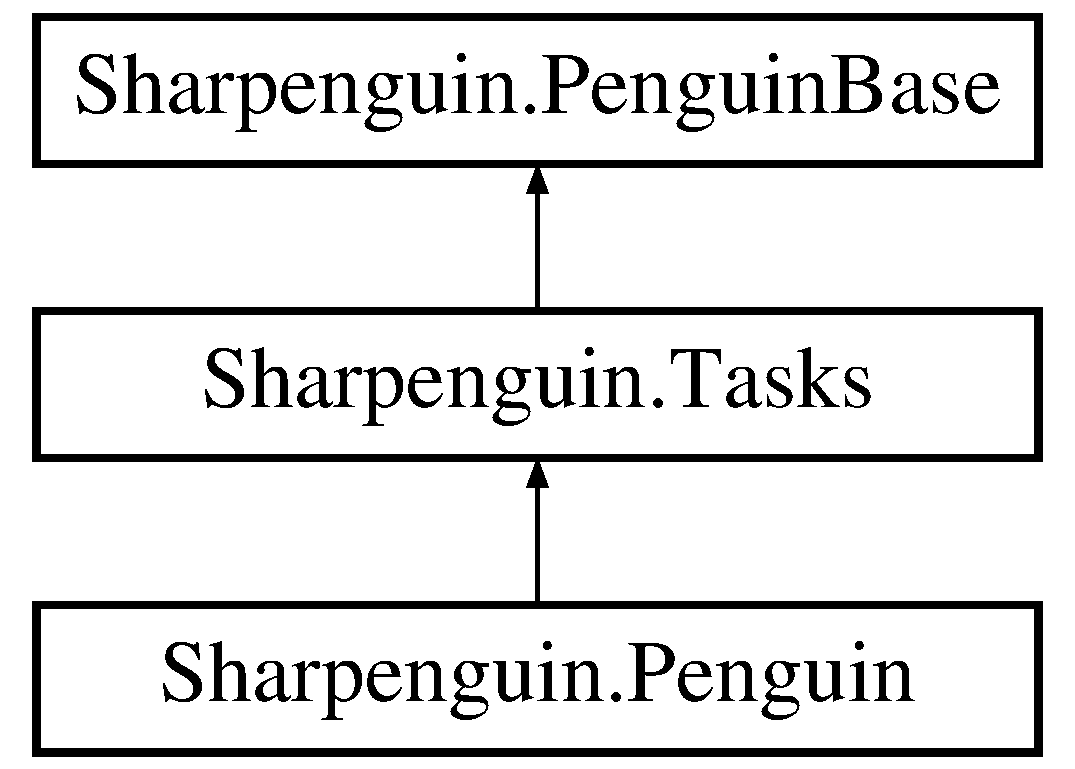
\includegraphics[height=3.000000cm]{classSharpenguin_1_1Tasks}
\end{center}
\end{figure}
\subsection*{Public Member Functions}
\begin{DoxyCompactItemize}
\item 
\hyperlink{classSharpenguin_1_1Tasks_ad11714a7d933773ab18d4bb2585edeee}{Tasks} ()
\item 
void \hyperlink{classSharpenguin_1_1Tasks_aded18ef49c423a750812df9dad65347f}{Send\-Message} (string str\-Message)
\item 
\hypertarget{classSharpenguin_1_1Tasks_abf3a4f9bdb323896e55c599a05f5eac8}{void {\bfseries Send\-Blocked} (string str\-Message)}\label{classSharpenguin_1_1Tasks_abf3a4f9bdb323896e55c599a05f5eac8}

\item 
bool \hyperlink{classSharpenguin_1_1Tasks_a2c6d78357cc26cb67b0f8af7872adb19}{Send\-Emote} (object obj\-Emote\-Id)
\item 
bool \hyperlink{classSharpenguin_1_1Tasks_acdb6387b11485a7e14c70dd421c76388}{Send\-Joke} (int int\-Joke)
\item 
bool \hyperlink{classSharpenguin_1_1Tasks_a1226e45b3561d9a0ab01575ad70a3622}{Send\-Safe} (int int\-Safe)
\item 
\hypertarget{classSharpenguin_1_1Tasks_a0fe79158b2c170853d3708449e9b0a3b}{void {\bfseries Send\-Line} (int int\-Message\-I\-D)}\label{classSharpenguin_1_1Tasks_a0fe79158b2c170853d3708449e9b0a3b}

\item 
\hypertarget{classSharpenguin_1_1Tasks_ad46067f2d4d94523038001511eb0a733}{void {\bfseries Send\-Quick} (int int\-Message\-I\-D)}\label{classSharpenguin_1_1Tasks_ad46067f2d4d94523038001511eb0a733}

\item 
void \hyperlink{classSharpenguin_1_1Tasks_a6c32c1c6f88de4fbd9cf85f2082569dd}{Send\-Guide} (int int\-Message\-I\-D)
\item 
void \hyperlink{classSharpenguin_1_1Tasks_a42de1c57af7ccf4d72a4a0acef7f35fb}{Send\-Position} (int int\-X, int int\-Y)
\item 
void \hyperlink{classSharpenguin_1_1Tasks_a7a0a319638d008133580d51b97c6dd69}{snow\-Ball} (int int\-X, int int\-Y)
\item 
void \hyperlink{classSharpenguin_1_1Tasks_a247a2b0d766f9320292ed5b50475a8a7}{Send\-Action} (int int\-Action\-I\-D)
\item 
void \hyperlink{classSharpenguin_1_1Tasks_ae2befef95a890b44ce44d9add9b80608}{Send\-Frame} (int int\-Frame\-I\-D)
\item 
void \hyperlink{classSharpenguin_1_1Tasks_aeff19dc4bd2712ffe0fc78e7cabde77a}{Send\-Mail} (int int\-Penguin\-I\-D, int int\-Card\-I\-D)
\item 
void \hyperlink{classSharpenguin_1_1Tasks_a7b357b1776e1fb44c13d94ca25d329cc}{find\-Buddy} (int int\-Penguin\-I\-D)
\item 
void \hyperlink{classSharpenguin_1_1Tasks_a4f7ba17e14837328ea7d5802bf42342a}{add\-Ignore} (int int\-Penguin\-I\-D)
\item 
void \hyperlink{classSharpenguin_1_1Tasks_a1839f7c13f64f974a04d183b7d594282}{remove\-Ignore} (int int\-Penguin\-I\-D)
\item 
void \hyperlink{classSharpenguin_1_1Tasks_a3d1346d64943ff53952720b3f937f42f}{add\-Item} (int int\-Item\-Id)
\item 
void \hyperlink{classSharpenguin_1_1Tasks_a8555c5e67357445329083acf44ae7059}{add\-Stamp} (int int\-Id)
\item 
void \hyperlink{classSharpenguin_1_1Tasks_ab45a306238a875d196c3fe4ddc9d99a0}{update\-Colour} (int int\-Item\-I\-D)
\item 
void \hyperlink{classSharpenguin_1_1Tasks_a039222d09a2ed544a40947a3fd11d129}{update\-Head} (int int\-Item\-I\-D)
\item 
void \hyperlink{classSharpenguin_1_1Tasks_aa24f1d630ed91477ac4303d0ff72f7a6}{update\-Face} (int int\-Item\-I\-D)
\item 
void \hyperlink{classSharpenguin_1_1Tasks_a9fee874da71ae90e0c0f56a37d522fe8}{update\-Neck} (int int\-Item\-I\-D)
\item 
void \hyperlink{classSharpenguin_1_1Tasks_a6df07df165c03d43ed90bf818aae1f6a}{update\-Body} (int int\-Item\-I\-D)
\item 
void \hyperlink{classSharpenguin_1_1Tasks_a1e2a3bcb87966bebde0202356174962c}{update\-Hand} (int int\-Item\-I\-D)
\item 
void \hyperlink{classSharpenguin_1_1Tasks_afcfff4673b77a152c39934505324e794}{update\-Feet} (int int\-Item\-I\-D)
\item 
void \hyperlink{classSharpenguin_1_1Tasks_a5dbd850a020d9d459eed99a8c45d8e75}{update\-Flag} (int int\-Item\-I\-D)
\item 
void \hyperlink{classSharpenguin_1_1Tasks_a28834ede17e7850508025bbed190a641}{update\-Photo} (int int\-Item\-I\-D)
\item 
\hypertarget{classSharpenguin_1_1Tasks_af9b7a0677366bfaeba38dcc5cb0d8bb5}{void {\bfseries update\-Remove} (int int\-Item\-I\-D)}\label{classSharpenguin_1_1Tasks_af9b7a0677366bfaeba38dcc5cb0d8bb5}

\item 
void \hyperlink{classSharpenguin_1_1Tasks_a29e019a91b08cb92c9fa7f3ba9f33776}{join\-Igloo} (int int\-Penguin\-I\-D)
\item 
void \hyperlink{classSharpenguin_1_1Tasks_aca9013fed2c6e6cf5e19771aae98531d}{open\-Newspaper} ()
\item 
void \hyperlink{classSharpenguin_1_1Tasks_afa6b3fb4e044dfaf6c9520b56d276dca}{close\-Newspaper} ()
\item 
void \hyperlink{classSharpenguin_1_1Tasks_ae4e482fa82fb3c02cae015f4ae9f527c}{get\-Coins} (int int\-Amount)
\item 
\hypertarget{classSharpenguin_1_1Tasks_a5518e385cb00ea50b63cf03035d31717}{void {\bfseries get\-Player} (int int\-Penguin\-I\-D)}\label{classSharpenguin_1_1Tasks_a5518e385cb00ea50b63cf03035d31717}

\item 
void \hyperlink{classSharpenguin_1_1Tasks_a2e667922c2df819ec504636ab8523f5a}{buy\-Puffle} (int int\-Puffle\-I\-D, string str\-Name)
\item 
void \hyperlink{classSharpenguin_1_1Tasks_af7ed0b413f925907983b7242441074c1}{join\-Game} (object obj\-Game\-Room)
\item 
void \hyperlink{classSharpenguin_1_1Tasks_ab6153b32f78f2a137bda915a3a35cecd}{request\-Epf\-Messages} ()
\item 
bool \hyperlink{classSharpenguin_1_1Tasks_ad71a7aec9611f9aaf9715a52bde33c04}{join\-Room} (object obj\-Room, int int\-X=0, int int\-Y=0)
\item 
void \hyperlink{classSharpenguin_1_1Tasks_a9ceb3ef96c8a645127c4353afbcc4560}{Send\-Phrase\-Message} (string str\-Id)
\item 
void \hyperlink{classSharpenguin_1_1Tasks_a5965355bcfb2fd527fa4436b34a1aeb7}{Send\-Join} (string str\-Login\-Key)
\item 
void \hyperlink{classSharpenguin_1_1Tasks_a2fd5289a96dc2a8466554e89fed6de97}{Send\-Get\-Inventory} ()
\end{DoxyCompactItemize}
\subsection*{Additional Inherited Members}


\subsection{Detailed Description}
An extension of \hyperlink{classSharpenguin_1_1PenguinBase}{Penguin\-Base} with all of the tasks you can perform on the Club \hyperlink{classSharpenguin_1_1Penguin}{Penguin} game servers. 

\subsection{Constructor \& Destructor Documentation}
\hypertarget{classSharpenguin_1_1Tasks_ad11714a7d933773ab18d4bb2585edeee}{\index{Sharpenguin\-::\-Tasks@{Sharpenguin\-::\-Tasks}!Tasks@{Tasks}}
\index{Tasks@{Tasks}!Sharpenguin::Tasks@{Sharpenguin\-::\-Tasks}}
\subsubsection[{Tasks}]{\setlength{\rightskip}{0pt plus 5cm}Sharpenguin.\-Tasks.\-Tasks (
\begin{DoxyParamCaption}
{}
\end{DoxyParamCaption}
)\hspace{0.3cm}{\ttfamily [inline]}}}\label{classSharpenguin_1_1Tasks_ad11714a7d933773ab18d4bb2585edeee}
Constructor, extended from the base class. 

\subsection{Member Function Documentation}
\hypertarget{classSharpenguin_1_1Tasks_a4f7ba17e14837328ea7d5802bf42342a}{\index{Sharpenguin\-::\-Tasks@{Sharpenguin\-::\-Tasks}!add\-Ignore@{add\-Ignore}}
\index{add\-Ignore@{add\-Ignore}!Sharpenguin::Tasks@{Sharpenguin\-::\-Tasks}}
\subsubsection[{add\-Ignore}]{\setlength{\rightskip}{0pt plus 5cm}void Sharpenguin.\-Tasks.\-add\-Ignore (
\begin{DoxyParamCaption}
\item[{int}]{int\-Penguin\-I\-D}
\end{DoxyParamCaption}
)\hspace{0.3cm}{\ttfamily [inline]}}}\label{classSharpenguin_1_1Tasks_a4f7ba17e14837328ea7d5802bf42342a}
Ignores a player by their id.


\begin{DoxyParams}{Parameters}
{\em int\-Penguin\-I\-D} & The id of the penguin to ignore. \\
\hline
\end{DoxyParams}
\hypertarget{classSharpenguin_1_1Tasks_a3d1346d64943ff53952720b3f937f42f}{\index{Sharpenguin\-::\-Tasks@{Sharpenguin\-::\-Tasks}!add\-Item@{add\-Item}}
\index{add\-Item@{add\-Item}!Sharpenguin::Tasks@{Sharpenguin\-::\-Tasks}}
\subsubsection[{add\-Item}]{\setlength{\rightskip}{0pt plus 5cm}void Sharpenguin.\-Tasks.\-add\-Item (
\begin{DoxyParamCaption}
\item[{int}]{int\-Item\-Id}
\end{DoxyParamCaption}
)\hspace{0.3cm}{\ttfamily [inline]}}}\label{classSharpenguin_1_1Tasks_a3d1346d64943ff53952720b3f937f42f}
Adds an item to the player's inventory.


\begin{DoxyParams}{Parameters}
{\em int\-Item\-Id} & Id of the item to add. \\
\hline
\end{DoxyParams}
\hypertarget{classSharpenguin_1_1Tasks_a8555c5e67357445329083acf44ae7059}{\index{Sharpenguin\-::\-Tasks@{Sharpenguin\-::\-Tasks}!add\-Stamp@{add\-Stamp}}
\index{add\-Stamp@{add\-Stamp}!Sharpenguin::Tasks@{Sharpenguin\-::\-Tasks}}
\subsubsection[{add\-Stamp}]{\setlength{\rightskip}{0pt plus 5cm}void Sharpenguin.\-Tasks.\-add\-Stamp (
\begin{DoxyParamCaption}
\item[{int}]{int\-Id}
\end{DoxyParamCaption}
)\hspace{0.3cm}{\ttfamily [inline]}}}\label{classSharpenguin_1_1Tasks_a8555c5e67357445329083acf44ae7059}
Adds a stamp -\/ W\-A\-R\-N\-I\-N\-G, Y\-O\-U M\-A\-Y B\-E B\-A\-N\-N\-E\-D. U\-S\-E W\-I\-T\-H C\-A\-U\-T\-I\-O\-N.


\begin{DoxyParams}{Parameters}
{\em int\-Id} & Id of the stamp to add. \\
\hline
\end{DoxyParams}
\hypertarget{classSharpenguin_1_1Tasks_a2e667922c2df819ec504636ab8523f5a}{\index{Sharpenguin\-::\-Tasks@{Sharpenguin\-::\-Tasks}!buy\-Puffle@{buy\-Puffle}}
\index{buy\-Puffle@{buy\-Puffle}!Sharpenguin::Tasks@{Sharpenguin\-::\-Tasks}}
\subsubsection[{buy\-Puffle}]{\setlength{\rightskip}{0pt plus 5cm}void Sharpenguin.\-Tasks.\-buy\-Puffle (
\begin{DoxyParamCaption}
\item[{int}]{int\-Puffle\-I\-D, }
\item[{string}]{str\-Name}
\end{DoxyParamCaption}
)\hspace{0.3cm}{\ttfamily [inline]}}}\label{classSharpenguin_1_1Tasks_a2e667922c2df819ec504636ab8523f5a}
Buys a new puffle.


\begin{DoxyParams}{Parameters}
{\em int\-Puffle\-I\-D} & The item id of the puffle. \\
\hline
{\em str\-Name} & The name of your puffle. \\
\hline
\end{DoxyParams}
\hypertarget{classSharpenguin_1_1Tasks_afa6b3fb4e044dfaf6c9520b56d276dca}{\index{Sharpenguin\-::\-Tasks@{Sharpenguin\-::\-Tasks}!close\-Newspaper@{close\-Newspaper}}
\index{close\-Newspaper@{close\-Newspaper}!Sharpenguin::Tasks@{Sharpenguin\-::\-Tasks}}
\subsubsection[{close\-Newspaper}]{\setlength{\rightskip}{0pt plus 5cm}void Sharpenguin.\-Tasks.\-close\-Newspaper (
\begin{DoxyParamCaption}
{}
\end{DoxyParamCaption}
)\hspace{0.3cm}{\ttfamily [inline]}}}\label{classSharpenguin_1_1Tasks_afa6b3fb4e044dfaf6c9520b56d276dca}
Closes the newspaper. \hypertarget{classSharpenguin_1_1Tasks_a7b357b1776e1fb44c13d94ca25d329cc}{\index{Sharpenguin\-::\-Tasks@{Sharpenguin\-::\-Tasks}!find\-Buddy@{find\-Buddy}}
\index{find\-Buddy@{find\-Buddy}!Sharpenguin::Tasks@{Sharpenguin\-::\-Tasks}}
\subsubsection[{find\-Buddy}]{\setlength{\rightskip}{0pt plus 5cm}void Sharpenguin.\-Tasks.\-find\-Buddy (
\begin{DoxyParamCaption}
\item[{int}]{int\-Penguin\-I\-D}
\end{DoxyParamCaption}
)\hspace{0.3cm}{\ttfamily [inline]}}}\label{classSharpenguin_1_1Tasks_a7b357b1776e1fb44c13d94ca25d329cc}
Finds a penguin by their I\-D.


\begin{DoxyParams}{Parameters}
{\em int\-Penguin\-I\-D} & The id of the penguin to find \\
\hline
\end{DoxyParams}
\hypertarget{classSharpenguin_1_1Tasks_ae4e482fa82fb3c02cae015f4ae9f527c}{\index{Sharpenguin\-::\-Tasks@{Sharpenguin\-::\-Tasks}!get\-Coins@{get\-Coins}}
\index{get\-Coins@{get\-Coins}!Sharpenguin::Tasks@{Sharpenguin\-::\-Tasks}}
\subsubsection[{get\-Coins}]{\setlength{\rightskip}{0pt plus 5cm}void Sharpenguin.\-Tasks.\-get\-Coins (
\begin{DoxyParamCaption}
\item[{int}]{int\-Amount}
\end{DoxyParamCaption}
)\hspace{0.3cm}{\ttfamily [inline]}}}\label{classSharpenguin_1_1Tasks_ae4e482fa82fb3c02cae015f4ae9f527c}
Gets coins from a game.


\begin{DoxyParams}{Parameters}
{\em int\-Amount} & Amount of coins to receive. \\
\hline
\end{DoxyParams}
\hypertarget{classSharpenguin_1_1Tasks_af7ed0b413f925907983b7242441074c1}{\index{Sharpenguin\-::\-Tasks@{Sharpenguin\-::\-Tasks}!join\-Game@{join\-Game}}
\index{join\-Game@{join\-Game}!Sharpenguin::Tasks@{Sharpenguin\-::\-Tasks}}
\subsubsection[{join\-Game}]{\setlength{\rightskip}{0pt plus 5cm}void Sharpenguin.\-Tasks.\-join\-Game (
\begin{DoxyParamCaption}
\item[{object}]{obj\-Game\-Room}
\end{DoxyParamCaption}
)\hspace{0.3cm}{\ttfamily [inline]}}}\label{classSharpenguin_1_1Tasks_af7ed0b413f925907983b7242441074c1}
Alias of join room, since the two are the same.


\begin{DoxyParams}{Parameters}
{\em int\-Game\-Room} & The id of the game's room. \\
\hline
\end{DoxyParams}
\hypertarget{classSharpenguin_1_1Tasks_a29e019a91b08cb92c9fa7f3ba9f33776}{\index{Sharpenguin\-::\-Tasks@{Sharpenguin\-::\-Tasks}!join\-Igloo@{join\-Igloo}}
\index{join\-Igloo@{join\-Igloo}!Sharpenguin::Tasks@{Sharpenguin\-::\-Tasks}}
\subsubsection[{join\-Igloo}]{\setlength{\rightskip}{0pt plus 5cm}void Sharpenguin.\-Tasks.\-join\-Igloo (
\begin{DoxyParamCaption}
\item[{int}]{int\-Penguin\-I\-D}
\end{DoxyParamCaption}
)\hspace{0.3cm}{\ttfamily [inline]}}}\label{classSharpenguin_1_1Tasks_a29e019a91b08cb92c9fa7f3ba9f33776}
Joins a player's igloo.


\begin{DoxyParams}{Parameters}
{\em int\-Penguin\-I\-D} & The id of the penguin who's igloo you wish to go to. \\
\hline
\end{DoxyParams}
\hypertarget{classSharpenguin_1_1Tasks_ad71a7aec9611f9aaf9715a52bde33c04}{\index{Sharpenguin\-::\-Tasks@{Sharpenguin\-::\-Tasks}!join\-Room@{join\-Room}}
\index{join\-Room@{join\-Room}!Sharpenguin::Tasks@{Sharpenguin\-::\-Tasks}}
\subsubsection[{join\-Room}]{\setlength{\rightskip}{0pt plus 5cm}bool Sharpenguin.\-Tasks.\-join\-Room (
\begin{DoxyParamCaption}
\item[{object}]{obj\-Room, }
\item[{int}]{int\-X = {\ttfamily 0}, }
\item[{int}]{int\-Y = {\ttfamily 0}}
\end{DoxyParamCaption}
)\hspace{0.3cm}{\ttfamily [inline]}}}\label{classSharpenguin_1_1Tasks_ad71a7aec9611f9aaf9715a52bde33c04}
Joins a room.


\begin{DoxyParams}{Parameters}
{\em obj\-Room} & The id, or name, of the room -\/ note, id is faster.\\
\hline
{\em int\-X} & The x position to enter the room. \\
\hline
{\em int\-Y} & The y position to enter the toom.\\
\hline
\end{DoxyParams}
\begin{DoxyReturn}{Returns}
T\-R\-U\-E if room exists, F\-A\-L\-S\-E if it does not. 
\end{DoxyReturn}
\hypertarget{classSharpenguin_1_1Tasks_aca9013fed2c6e6cf5e19771aae98531d}{\index{Sharpenguin\-::\-Tasks@{Sharpenguin\-::\-Tasks}!open\-Newspaper@{open\-Newspaper}}
\index{open\-Newspaper@{open\-Newspaper}!Sharpenguin::Tasks@{Sharpenguin\-::\-Tasks}}
\subsubsection[{open\-Newspaper}]{\setlength{\rightskip}{0pt plus 5cm}void Sharpenguin.\-Tasks.\-open\-Newspaper (
\begin{DoxyParamCaption}
{}
\end{DoxyParamCaption}
)\hspace{0.3cm}{\ttfamily [inline]}}}\label{classSharpenguin_1_1Tasks_aca9013fed2c6e6cf5e19771aae98531d}
Opens the newspaper. \hypertarget{classSharpenguin_1_1Tasks_a1839f7c13f64f974a04d183b7d594282}{\index{Sharpenguin\-::\-Tasks@{Sharpenguin\-::\-Tasks}!remove\-Ignore@{remove\-Ignore}}
\index{remove\-Ignore@{remove\-Ignore}!Sharpenguin::Tasks@{Sharpenguin\-::\-Tasks}}
\subsubsection[{remove\-Ignore}]{\setlength{\rightskip}{0pt plus 5cm}void Sharpenguin.\-Tasks.\-remove\-Ignore (
\begin{DoxyParamCaption}
\item[{int}]{int\-Penguin\-I\-D}
\end{DoxyParamCaption}
)\hspace{0.3cm}{\ttfamily [inline]}}}\label{classSharpenguin_1_1Tasks_a1839f7c13f64f974a04d183b7d594282}
Removes player from ignore list bt their id.


\begin{DoxyParams}{Parameters}
{\em int\-Penguin\-I\-D} & The id of the penguin to ignore. \\
\hline
\end{DoxyParams}
\hypertarget{classSharpenguin_1_1Tasks_ab6153b32f78f2a137bda915a3a35cecd}{\index{Sharpenguin\-::\-Tasks@{Sharpenguin\-::\-Tasks}!request\-Epf\-Messages@{request\-Epf\-Messages}}
\index{request\-Epf\-Messages@{request\-Epf\-Messages}!Sharpenguin::Tasks@{Sharpenguin\-::\-Tasks}}
\subsubsection[{request\-Epf\-Messages}]{\setlength{\rightskip}{0pt plus 5cm}void Sharpenguin.\-Tasks.\-request\-Epf\-Messages (
\begin{DoxyParamCaption}
{}
\end{DoxyParamCaption}
)\hspace{0.3cm}{\ttfamily [inline]}}}\label{classSharpenguin_1_1Tasks_ab6153b32f78f2a137bda915a3a35cecd}
Requests E\-P\-F messages from the server.

Requests E\-P\-F messages, which are usually displayed on the E\-P\-F phone. \hypertarget{classSharpenguin_1_1Tasks_a247a2b0d766f9320292ed5b50475a8a7}{\index{Sharpenguin\-::\-Tasks@{Sharpenguin\-::\-Tasks}!Send\-Action@{Send\-Action}}
\index{Send\-Action@{Send\-Action}!Sharpenguin::Tasks@{Sharpenguin\-::\-Tasks}}
\subsubsection[{Send\-Action}]{\setlength{\rightskip}{0pt plus 5cm}void Sharpenguin.\-Tasks.\-Send\-Action (
\begin{DoxyParamCaption}
\item[{int}]{int\-Action\-I\-D}
\end{DoxyParamCaption}
)\hspace{0.3cm}{\ttfamily [inline]}}}\label{classSharpenguin_1_1Tasks_a247a2b0d766f9320292ed5b50475a8a7}
Send an action to the room.


\begin{DoxyParams}{Parameters}
{\em int\-Action\-I\-D} & The id of the action to Send. \\
\hline
\end{DoxyParams}
\hypertarget{classSharpenguin_1_1Tasks_a2c6d78357cc26cb67b0f8af7872adb19}{\index{Sharpenguin\-::\-Tasks@{Sharpenguin\-::\-Tasks}!Send\-Emote@{Send\-Emote}}
\index{Send\-Emote@{Send\-Emote}!Sharpenguin::Tasks@{Sharpenguin\-::\-Tasks}}
\subsubsection[{Send\-Emote}]{\setlength{\rightskip}{0pt plus 5cm}bool Sharpenguin.\-Tasks.\-Send\-Emote (
\begin{DoxyParamCaption}
\item[{object}]{obj\-Emote\-Id}
\end{DoxyParamCaption}
)\hspace{0.3cm}{\ttfamily [inline]}}}\label{classSharpenguin_1_1Tasks_a2c6d78357cc26cb67b0f8af7872adb19}
Sends an emoticon to the room.


\begin{DoxyParams}{Parameters}
{\em obj\-Emote\-Id} & The id, or text representation, of the emote. (note, id is faster.)\\
\hline
\end{DoxyParams}
\begin{DoxyReturn}{Returns}
T\-R\-U\-E if emote exists, F\-A\-L\-S\-E if it does not. 
\end{DoxyReturn}
\hypertarget{classSharpenguin_1_1Tasks_ae2befef95a890b44ce44d9add9b80608}{\index{Sharpenguin\-::\-Tasks@{Sharpenguin\-::\-Tasks}!Send\-Frame@{Send\-Frame}}
\index{Send\-Frame@{Send\-Frame}!Sharpenguin::Tasks@{Sharpenguin\-::\-Tasks}}
\subsubsection[{Send\-Frame}]{\setlength{\rightskip}{0pt plus 5cm}void Sharpenguin.\-Tasks.\-Send\-Frame (
\begin{DoxyParamCaption}
\item[{int}]{int\-Frame\-I\-D}
\end{DoxyParamCaption}
)\hspace{0.3cm}{\ttfamily [inline]}}}\label{classSharpenguin_1_1Tasks_ae2befef95a890b44ce44d9add9b80608}
Sends a frame to the room.


\begin{DoxyParams}{Parameters}
{\em int\-Frame\-I\-D} & The id of the frame to Send. \\
\hline
\end{DoxyParams}
\hypertarget{classSharpenguin_1_1Tasks_a2fd5289a96dc2a8466554e89fed6de97}{\index{Sharpenguin\-::\-Tasks@{Sharpenguin\-::\-Tasks}!Send\-Get\-Inventory@{Send\-Get\-Inventory}}
\index{Send\-Get\-Inventory@{Send\-Get\-Inventory}!Sharpenguin::Tasks@{Sharpenguin\-::\-Tasks}}
\subsubsection[{Send\-Get\-Inventory}]{\setlength{\rightskip}{0pt plus 5cm}void Sharpenguin.\-Tasks.\-Send\-Get\-Inventory (
\begin{DoxyParamCaption}
{}
\end{DoxyParamCaption}
)\hspace{0.3cm}{\ttfamily [inline]}}}\label{classSharpenguin_1_1Tasks_a2fd5289a96dc2a8466554e89fed6de97}
Asks the server for your inventory.


\begin{DoxyParams}{Parameters}
{\em str\-Login\-Key} & The login key we were given by the login server. \\
\hline
\end{DoxyParams}
\hypertarget{classSharpenguin_1_1Tasks_a6c32c1c6f88de4fbd9cf85f2082569dd}{\index{Sharpenguin\-::\-Tasks@{Sharpenguin\-::\-Tasks}!Send\-Guide@{Send\-Guide}}
\index{Send\-Guide@{Send\-Guide}!Sharpenguin::Tasks@{Sharpenguin\-::\-Tasks}}
\subsubsection[{Send\-Guide}]{\setlength{\rightskip}{0pt plus 5cm}void Sharpenguin.\-Tasks.\-Send\-Guide (
\begin{DoxyParamCaption}
\item[{int}]{int\-Message\-I\-D}
\end{DoxyParamCaption}
)\hspace{0.3cm}{\ttfamily [inline]}}}\label{classSharpenguin_1_1Tasks_a6c32c1c6f88de4fbd9cf85f2082569dd}
Sends a tour guide message to the server.


\begin{DoxyParams}{Parameters}
{\em int\-Message\-I\-D} & The id of the tour guide message. \\
\hline
\end{DoxyParams}
\hypertarget{classSharpenguin_1_1Tasks_a5965355bcfb2fd527fa4436b34a1aeb7}{\index{Sharpenguin\-::\-Tasks@{Sharpenguin\-::\-Tasks}!Send\-Join@{Send\-Join}}
\index{Send\-Join@{Send\-Join}!Sharpenguin::Tasks@{Sharpenguin\-::\-Tasks}}
\subsubsection[{Send\-Join}]{\setlength{\rightskip}{0pt plus 5cm}void Sharpenguin.\-Tasks.\-Send\-Join (
\begin{DoxyParamCaption}
\item[{string}]{str\-Login\-Key}
\end{DoxyParamCaption}
)\hspace{0.3cm}{\ttfamily [inline]}}}\label{classSharpenguin_1_1Tasks_a5965355bcfb2fd527fa4436b34a1aeb7}
Sends a join packet to a game server.


\begin{DoxyParams}{Parameters}
{\em str\-Login\-Key} & The login key we were given by the login server. \\
\hline
\end{DoxyParams}
\hypertarget{classSharpenguin_1_1Tasks_acdb6387b11485a7e14c70dd421c76388}{\index{Sharpenguin\-::\-Tasks@{Sharpenguin\-::\-Tasks}!Send\-Joke@{Send\-Joke}}
\index{Send\-Joke@{Send\-Joke}!Sharpenguin::Tasks@{Sharpenguin\-::\-Tasks}}
\subsubsection[{Send\-Joke}]{\setlength{\rightskip}{0pt plus 5cm}bool Sharpenguin.\-Tasks.\-Send\-Joke (
\begin{DoxyParamCaption}
\item[{int}]{int\-Joke}
\end{DoxyParamCaption}
)\hspace{0.3cm}{\ttfamily [inline]}}}\label{classSharpenguin_1_1Tasks_acdb6387b11485a7e14c70dd421c76388}
Sends a joke to the room.


\begin{DoxyParams}{Parameters}
{\em int\-Joke} & The id of the joke.\\
\hline
\end{DoxyParams}
\begin{DoxyReturn}{Returns}
T\-R\-U\-E if the joke exists, F\-A\-L\-S\-E if it does not. 
\end{DoxyReturn}
\hypertarget{classSharpenguin_1_1Tasks_aeff19dc4bd2712ffe0fc78e7cabde77a}{\index{Sharpenguin\-::\-Tasks@{Sharpenguin\-::\-Tasks}!Send\-Mail@{Send\-Mail}}
\index{Send\-Mail@{Send\-Mail}!Sharpenguin::Tasks@{Sharpenguin\-::\-Tasks}}
\subsubsection[{Send\-Mail}]{\setlength{\rightskip}{0pt plus 5cm}void Sharpenguin.\-Tasks.\-Send\-Mail (
\begin{DoxyParamCaption}
\item[{int}]{int\-Penguin\-I\-D, }
\item[{int}]{int\-Card\-I\-D}
\end{DoxyParamCaption}
)\hspace{0.3cm}{\ttfamily [inline]}}}\label{classSharpenguin_1_1Tasks_aeff19dc4bd2712ffe0fc78e7cabde77a}
Sends a post card to a penguin.


\begin{DoxyParams}{Parameters}
{\em int\-Penguin\-I\-D} & The id of the penguin to Send to. \\
\hline
{\em int\-Card\-I\-D} & The id of the card to Send. \\
\hline
\end{DoxyParams}
\hypertarget{classSharpenguin_1_1Tasks_aded18ef49c423a750812df9dad65347f}{\index{Sharpenguin\-::\-Tasks@{Sharpenguin\-::\-Tasks}!Send\-Message@{Send\-Message}}
\index{Send\-Message@{Send\-Message}!Sharpenguin::Tasks@{Sharpenguin\-::\-Tasks}}
\subsubsection[{Send\-Message}]{\setlength{\rightskip}{0pt plus 5cm}void Sharpenguin.\-Tasks.\-Send\-Message (
\begin{DoxyParamCaption}
\item[{string}]{str\-Message}
\end{DoxyParamCaption}
)\hspace{0.3cm}{\ttfamily [inline]}}}\label{classSharpenguin_1_1Tasks_aded18ef49c423a750812df9dad65347f}
Sends a message to everyone in the room.


\begin{DoxyParams}{Parameters}
{\em str\-Message} & The message to Send. \\
\hline
\end{DoxyParams}
\hypertarget{classSharpenguin_1_1Tasks_a9ceb3ef96c8a645127c4353afbcc4560}{\index{Sharpenguin\-::\-Tasks@{Sharpenguin\-::\-Tasks}!Send\-Phrase\-Message@{Send\-Phrase\-Message}}
\index{Send\-Phrase\-Message@{Send\-Phrase\-Message}!Sharpenguin::Tasks@{Sharpenguin\-::\-Tasks}}
\subsubsection[{Send\-Phrase\-Message}]{\setlength{\rightskip}{0pt plus 5cm}void Sharpenguin.\-Tasks.\-Send\-Phrase\-Message (
\begin{DoxyParamCaption}
\item[{string}]{str\-Id}
\end{DoxyParamCaption}
)\hspace{0.3cm}{\ttfamily [inline]}}}\label{classSharpenguin_1_1Tasks_a9ceb3ef96c8a645127c4353afbcc4560}
Sends a phrase message to the room


\begin{DoxyParams}{Parameters}
{\em str\-Id} & I\-D of the phrase. \\
\hline
\end{DoxyParams}
\hypertarget{classSharpenguin_1_1Tasks_a42de1c57af7ccf4d72a4a0acef7f35fb}{\index{Sharpenguin\-::\-Tasks@{Sharpenguin\-::\-Tasks}!Send\-Position@{Send\-Position}}
\index{Send\-Position@{Send\-Position}!Sharpenguin::Tasks@{Sharpenguin\-::\-Tasks}}
\subsubsection[{Send\-Position}]{\setlength{\rightskip}{0pt plus 5cm}void Sharpenguin.\-Tasks.\-Send\-Position (
\begin{DoxyParamCaption}
\item[{int}]{int\-X, }
\item[{int}]{int\-Y}
\end{DoxyParamCaption}
)\hspace{0.3cm}{\ttfamily [inline]}}}\label{classSharpenguin_1_1Tasks_a42de1c57af7ccf4d72a4a0acef7f35fb}
Sends a new player position to the room, effectively moving your player.


\begin{DoxyParams}{Parameters}
{\em int\-X} & X Position to move to. \\
\hline
{\em int\-Y} & Y Position to move to. \\
\hline
\end{DoxyParams}
\hypertarget{classSharpenguin_1_1Tasks_a1226e45b3561d9a0ab01575ad70a3622}{\index{Sharpenguin\-::\-Tasks@{Sharpenguin\-::\-Tasks}!Send\-Safe@{Send\-Safe}}
\index{Send\-Safe@{Send\-Safe}!Sharpenguin::Tasks@{Sharpenguin\-::\-Tasks}}
\subsubsection[{Send\-Safe}]{\setlength{\rightskip}{0pt plus 5cm}bool Sharpenguin.\-Tasks.\-Send\-Safe (
\begin{DoxyParamCaption}
\item[{int}]{int\-Safe}
\end{DoxyParamCaption}
)\hspace{0.3cm}{\ttfamily [inline]}}}\label{classSharpenguin_1_1Tasks_a1226e45b3561d9a0ab01575ad70a3622}
Sends a safe message to the room.


\begin{DoxyParams}{Parameters}
{\em int\-Safe} & The id of the safe message.\\
\hline
\end{DoxyParams}
\begin{DoxyReturn}{Returns}
T\-R\-U\-E if the message exists, F\-A\-L\-S\-E if it does not. 
\end{DoxyReturn}
\hypertarget{classSharpenguin_1_1Tasks_a7a0a319638d008133580d51b97c6dd69}{\index{Sharpenguin\-::\-Tasks@{Sharpenguin\-::\-Tasks}!snow\-Ball@{snow\-Ball}}
\index{snow\-Ball@{snow\-Ball}!Sharpenguin::Tasks@{Sharpenguin\-::\-Tasks}}
\subsubsection[{snow\-Ball}]{\setlength{\rightskip}{0pt plus 5cm}void Sharpenguin.\-Tasks.\-snow\-Ball (
\begin{DoxyParamCaption}
\item[{int}]{int\-X, }
\item[{int}]{int\-Y}
\end{DoxyParamCaption}
)\hspace{0.3cm}{\ttfamily [inline]}}}\label{classSharpenguin_1_1Tasks_a7a0a319638d008133580d51b97c6dd69}
Throws a snowball.

Throws a snowball to the specified x and y position.


\begin{DoxyParams}{Parameters}
{\em int\-X} & The x position to throw the snowball. \\
\hline
{\em int\-Y} & The y position to throw the snowball. \\
\hline
\end{DoxyParams}
\hypertarget{classSharpenguin_1_1Tasks_a6df07df165c03d43ed90bf818aae1f6a}{\index{Sharpenguin\-::\-Tasks@{Sharpenguin\-::\-Tasks}!update\-Body@{update\-Body}}
\index{update\-Body@{update\-Body}!Sharpenguin::Tasks@{Sharpenguin\-::\-Tasks}}
\subsubsection[{update\-Body}]{\setlength{\rightskip}{0pt plus 5cm}void Sharpenguin.\-Tasks.\-update\-Body (
\begin{DoxyParamCaption}
\item[{int}]{int\-Item\-I\-D}
\end{DoxyParamCaption}
)\hspace{0.3cm}{\ttfamily [inline]}}}\label{classSharpenguin_1_1Tasks_a6df07df165c03d43ed90bf818aae1f6a}
Change's the player's body item.


\begin{DoxyParams}{Parameters}
{\em int\-Item\-I\-D} & The id of the body item to wear. \\
\hline
\end{DoxyParams}
\hypertarget{classSharpenguin_1_1Tasks_ab45a306238a875d196c3fe4ddc9d99a0}{\index{Sharpenguin\-::\-Tasks@{Sharpenguin\-::\-Tasks}!update\-Colour@{update\-Colour}}
\index{update\-Colour@{update\-Colour}!Sharpenguin::Tasks@{Sharpenguin\-::\-Tasks}}
\subsubsection[{update\-Colour}]{\setlength{\rightskip}{0pt plus 5cm}void Sharpenguin.\-Tasks.\-update\-Colour (
\begin{DoxyParamCaption}
\item[{int}]{int\-Item\-I\-D}
\end{DoxyParamCaption}
)\hspace{0.3cm}{\ttfamily [inline]}}}\label{classSharpenguin_1_1Tasks_ab45a306238a875d196c3fe4ddc9d99a0}
Change's the penguin's colour.


\begin{DoxyParams}{Parameters}
{\em int\-Item\-I\-D} & The id of the colour to change to. \\
\hline
\end{DoxyParams}
\hypertarget{classSharpenguin_1_1Tasks_aa24f1d630ed91477ac4303d0ff72f7a6}{\index{Sharpenguin\-::\-Tasks@{Sharpenguin\-::\-Tasks}!update\-Face@{update\-Face}}
\index{update\-Face@{update\-Face}!Sharpenguin::Tasks@{Sharpenguin\-::\-Tasks}}
\subsubsection[{update\-Face}]{\setlength{\rightskip}{0pt plus 5cm}void Sharpenguin.\-Tasks.\-update\-Face (
\begin{DoxyParamCaption}
\item[{int}]{int\-Item\-I\-D}
\end{DoxyParamCaption}
)\hspace{0.3cm}{\ttfamily [inline]}}}\label{classSharpenguin_1_1Tasks_aa24f1d630ed91477ac4303d0ff72f7a6}
Change's the player's face item.


\begin{DoxyParams}{Parameters}
{\em int\-Item\-I\-D} & The id of the face item to wear. \\
\hline
\end{DoxyParams}
\hypertarget{classSharpenguin_1_1Tasks_afcfff4673b77a152c39934505324e794}{\index{Sharpenguin\-::\-Tasks@{Sharpenguin\-::\-Tasks}!update\-Feet@{update\-Feet}}
\index{update\-Feet@{update\-Feet}!Sharpenguin::Tasks@{Sharpenguin\-::\-Tasks}}
\subsubsection[{update\-Feet}]{\setlength{\rightskip}{0pt plus 5cm}void Sharpenguin.\-Tasks.\-update\-Feet (
\begin{DoxyParamCaption}
\item[{int}]{int\-Item\-I\-D}
\end{DoxyParamCaption}
)\hspace{0.3cm}{\ttfamily [inline]}}}\label{classSharpenguin_1_1Tasks_afcfff4673b77a152c39934505324e794}
Change's the player's feet item.


\begin{DoxyParams}{Parameters}
{\em int\-Item\-I\-D} & The id of the feet item to wear. \\
\hline
\end{DoxyParams}
\hypertarget{classSharpenguin_1_1Tasks_a5dbd850a020d9d459eed99a8c45d8e75}{\index{Sharpenguin\-::\-Tasks@{Sharpenguin\-::\-Tasks}!update\-Flag@{update\-Flag}}
\index{update\-Flag@{update\-Flag}!Sharpenguin::Tasks@{Sharpenguin\-::\-Tasks}}
\subsubsection[{update\-Flag}]{\setlength{\rightskip}{0pt plus 5cm}void Sharpenguin.\-Tasks.\-update\-Flag (
\begin{DoxyParamCaption}
\item[{int}]{int\-Item\-I\-D}
\end{DoxyParamCaption}
)\hspace{0.3cm}{\ttfamily [inline]}}}\label{classSharpenguin_1_1Tasks_a5dbd850a020d9d459eed99a8c45d8e75}
Change's the player's flag item.


\begin{DoxyParams}{Parameters}
{\em int\-Item\-I\-D} & The id of the flag item to wear. \\
\hline
\end{DoxyParams}
\hypertarget{classSharpenguin_1_1Tasks_a1e2a3bcb87966bebde0202356174962c}{\index{Sharpenguin\-::\-Tasks@{Sharpenguin\-::\-Tasks}!update\-Hand@{update\-Hand}}
\index{update\-Hand@{update\-Hand}!Sharpenguin::Tasks@{Sharpenguin\-::\-Tasks}}
\subsubsection[{update\-Hand}]{\setlength{\rightskip}{0pt plus 5cm}void Sharpenguin.\-Tasks.\-update\-Hand (
\begin{DoxyParamCaption}
\item[{int}]{int\-Item\-I\-D}
\end{DoxyParamCaption}
)\hspace{0.3cm}{\ttfamily [inline]}}}\label{classSharpenguin_1_1Tasks_a1e2a3bcb87966bebde0202356174962c}
Change's the player's hand item.


\begin{DoxyParams}{Parameters}
{\em int\-Item\-I\-D} & The id of the hand item to wear. \\
\hline
\end{DoxyParams}
\hypertarget{classSharpenguin_1_1Tasks_a039222d09a2ed544a40947a3fd11d129}{\index{Sharpenguin\-::\-Tasks@{Sharpenguin\-::\-Tasks}!update\-Head@{update\-Head}}
\index{update\-Head@{update\-Head}!Sharpenguin::Tasks@{Sharpenguin\-::\-Tasks}}
\subsubsection[{update\-Head}]{\setlength{\rightskip}{0pt plus 5cm}void Sharpenguin.\-Tasks.\-update\-Head (
\begin{DoxyParamCaption}
\item[{int}]{int\-Item\-I\-D}
\end{DoxyParamCaption}
)\hspace{0.3cm}{\ttfamily [inline]}}}\label{classSharpenguin_1_1Tasks_a039222d09a2ed544a40947a3fd11d129}
Change's the player's head item.


\begin{DoxyParams}{Parameters}
{\em int\-Item\-I\-D} & The id of the head item to wear. \\
\hline
\end{DoxyParams}
\hypertarget{classSharpenguin_1_1Tasks_a9fee874da71ae90e0c0f56a37d522fe8}{\index{Sharpenguin\-::\-Tasks@{Sharpenguin\-::\-Tasks}!update\-Neck@{update\-Neck}}
\index{update\-Neck@{update\-Neck}!Sharpenguin::Tasks@{Sharpenguin\-::\-Tasks}}
\subsubsection[{update\-Neck}]{\setlength{\rightskip}{0pt plus 5cm}void Sharpenguin.\-Tasks.\-update\-Neck (
\begin{DoxyParamCaption}
\item[{int}]{int\-Item\-I\-D}
\end{DoxyParamCaption}
)\hspace{0.3cm}{\ttfamily [inline]}}}\label{classSharpenguin_1_1Tasks_a9fee874da71ae90e0c0f56a37d522fe8}
Change's the player's neck item.


\begin{DoxyParams}{Parameters}
{\em int\-Item\-I\-D} & The id of the neck item to wear. \\
\hline
\end{DoxyParams}
\hypertarget{classSharpenguin_1_1Tasks_a28834ede17e7850508025bbed190a641}{\index{Sharpenguin\-::\-Tasks@{Sharpenguin\-::\-Tasks}!update\-Photo@{update\-Photo}}
\index{update\-Photo@{update\-Photo}!Sharpenguin::Tasks@{Sharpenguin\-::\-Tasks}}
\subsubsection[{update\-Photo}]{\setlength{\rightskip}{0pt plus 5cm}void Sharpenguin.\-Tasks.\-update\-Photo (
\begin{DoxyParamCaption}
\item[{int}]{int\-Item\-I\-D}
\end{DoxyParamCaption}
)\hspace{0.3cm}{\ttfamily [inline]}}}\label{classSharpenguin_1_1Tasks_a28834ede17e7850508025bbed190a641}
Change's the player's photo item.


\begin{DoxyParams}{Parameters}
{\em int\-Item\-I\-D} & The id of the photo item to wear. \\
\hline
\end{DoxyParams}


The documentation for this class was generated from the following file\-:\begin{DoxyCompactItemize}
\item 
Tasks.\-cs\end{DoxyCompactItemize}

\hypertarget{classSharpenguin_1_1Xt_1_1XtParser}{\section{Sharpenguin.\-Xt.\-Xt\-Parser Class Reference}
\label{classSharpenguin_1_1Xt_1_1XtParser}\index{Sharpenguin.\-Xt.\-Xt\-Parser@{Sharpenguin.\-Xt.\-Xt\-Parser}}
}
\subsection*{Public Member Functions}
\begin{DoxyCompactItemize}
\item 
void \hyperlink{classSharpenguin_1_1Xt_1_1XtParser_a7f2d2d3ca37839e4a0315e8016886f7f}{Load\-Xt} (string str\-Data)
\end{DoxyCompactItemize}
\subsection*{Properties}
\begin{DoxyCompactItemize}
\item 
\hypertarget{classSharpenguin_1_1Xt_1_1XtParser_a3133f881cf40c91334824bce42ae4fdb}{int \hyperlink{classSharpenguin_1_1Xt_1_1XtParser_a3133f881cf40c91334824bce42ae4fdb}{Room}\hspace{0.3cm}{\ttfamily  \mbox{[}get\mbox{]}}}\label{classSharpenguin_1_1Xt_1_1XtParser_a3133f881cf40c91334824bce42ae4fdb}

\begin{DoxyCompactList}\small\item\em Gets the I\-D of the room this \hyperlink{namespaceSharpenguin_1_1Xt}{Xt} string came from (Internal Room). \end{DoxyCompactList}\item 
\hypertarget{classSharpenguin_1_1Xt_1_1XtParser_a6fb17caa59babd67acdcafc397cb563a}{string \hyperlink{classSharpenguin_1_1Xt_1_1XtParser_a6fb17caa59babd67acdcafc397cb563a}{Command}\hspace{0.3cm}{\ttfamily  \mbox{[}get\mbox{]}}}\label{classSharpenguin_1_1Xt_1_1XtParser_a6fb17caa59babd67acdcafc397cb563a}

\begin{DoxyCompactList}\small\item\em Gets the command of the \hyperlink{namespaceSharpenguin_1_1Xt}{Xt} string. \end{DoxyCompactList}\item 
\hypertarget{classSharpenguin_1_1Xt_1_1XtParser_a66f571aaabb838b143969f36ad797f92}{string\mbox{[}$\,$\mbox{]} \hyperlink{classSharpenguin_1_1Xt_1_1XtParser_a66f571aaabb838b143969f36ad797f92}{Arguments}\hspace{0.3cm}{\ttfamily  \mbox{[}get\mbox{]}}}\label{classSharpenguin_1_1Xt_1_1XtParser_a66f571aaabb838b143969f36ad797f92}

\begin{DoxyCompactList}\small\item\em Gets the arguments of the \hyperlink{namespaceSharpenguin_1_1Xt}{Xt} string. \end{DoxyCompactList}\end{DoxyCompactItemize}


\subsection{Detailed Description}
Parses xt packets for easier handling. 

\subsection{Member Function Documentation}
\hypertarget{classSharpenguin_1_1Xt_1_1XtParser_a7f2d2d3ca37839e4a0315e8016886f7f}{\index{Sharpenguin\-::\-Xt\-::\-Xt\-Parser@{Sharpenguin\-::\-Xt\-::\-Xt\-Parser}!Load\-Xt@{Load\-Xt}}
\index{Load\-Xt@{Load\-Xt}!Sharpenguin::Xt::XtParser@{Sharpenguin\-::\-Xt\-::\-Xt\-Parser}}
\subsubsection[{Load\-Xt}]{\setlength{\rightskip}{0pt plus 5cm}void Sharpenguin.\-Xt.\-Xt\-Parser.\-Load\-Xt (
\begin{DoxyParamCaption}
\item[{string}]{str\-Data}
\end{DoxyParamCaption}
)\hspace{0.3cm}{\ttfamily [inline]}}}\label{classSharpenguin_1_1Xt_1_1XtParser_a7f2d2d3ca37839e4a0315e8016886f7f}
Loads an xt string into the object.


\begin{DoxyParams}{Parameters}
{\em str\-Data} & The xt string. \\
\hline
\end{DoxyParams}


The documentation for this class was generated from the following file\-:\begin{DoxyCompactItemize}
\item 
Xt\-Parser.\-cs\end{DoxyCompactItemize}

\printindex
\end{document}
